%******************** 导言区 ********************%
\documentclass[twoside]{ctexbook}
% 定义文档类型，这里统一使用中文书籍类别，即"ctexbook"

\title{基础物理学B（1）\quad 知识点整理}

%================= 参考标题 =================%
% 工科数学分析（2）\\Mathematical Analysis for Engineering (2)
% 基础物理学B（1）\\Fundamental Physics B（1）
% 人工智能导论\\Introduction to Artificial Intelligence
% 数学分析进阶\\Advanced Mathematical Analysis for Engineering
% C程序设计进阶\\C Programming: Principles and Methods
% 大学化学\\College Chemistry 

\author{\kaishu \zihao{4}冯如书院学业支持中心学习部}
% 作者之间一定要用"\and "连接，否则名字会连到一起！

\date{2024--2025学年春季学期}
% 后续可能改为“冯如学业支持与科创教育中心学业支持部”


%================= 基础宏包 =================%
\usepackage{amsmath, amsthm, amssymb}      
% 数学公式核心支持
\usepackage[colorlinks, bookmarksnumbered]{hyperref} 
% 智能引用
\usepackage{tcolorbox}
% 美化定理框
\tcbuselibrary{skins,breakable} 
% 加载额外库以支持分页等更多功能
\usepackage{marginnote}                    
% 旁注系统
\usepackage[backend=biber, style=gb7714-2015]{biblatex} 
% 国标参考文献
\usepackage{booktabs}                      
% 专业表格
\usepackage{multirow}   
\usepackage{multicol}                   
% 复杂表格，合并单元格
\usepackage{tikz}                          
% 矢量绘图
\usepackage{enumitem}                      
% 列表控制
\usepackage{balance}
% 一页多栏平衡分布
\usepackage{lscape}
% 局部版面转置，用于过宽部分的转向
\usepackage{graphicx}
% 插图
\usepackage{wrapfig}
% 文字包围图表
\usepackage{textcomp}
% 特殊符号
\usepackage{xcolor}
% 控制颜色
\usepackage{caption}
% 图表标题
\usepackage{siunitx}
% 国际单位制
\usepackage{longtable}
% 长表格
\usepackage{mathrsfs}
% 特殊字体
\usepackage{bm}
% 加粗斜体
\usepackage{background}
%背景水印
\usetikzlibrary{calc}
\usepackage{watermark}

%================= 页面布局 =================%
\usepackage[paper=a4paper, 
    left=3cm, right=2.5cm, 
    top=2.5cm, bottom=2.5cm, 
    marginparwidth=3cm, 
    marginparsep=0.8cm]{geometry}

%================= 定理环境 =================%
\theoremstyle{plain}
\newtheorem{theorem}{定理}[chapter]
\newtheorem{lemma}[theorem]{引理}
\newtheorem{proposition}[theorem]{命题}

\theoremstyle{definition}
\newtheorem{definition}{定义}[chapter]
\newtheorem{example}{示例}[chapter]
\newtheorem{exercise}{习题}[section]

\theoremstyle{remark}
\newtheorem*{remark}{批注}
\newtheorem*{note}{注意}
\newtheorem*{supplement}{补充}
%================= 知识框样式 =================%
\tcbuselibrary{skins, theorems}
\newtcbtheorem[auto counter, number within=chapter]{knowledge}{知识要点}%
{enhanced, colframe=blue!75, colback=blue!5, 
boxrule=1pt, arc=3mm, fonttitle=\bfseries}{th}

\newtcbtheorem[auto counter, number within=chapter]{attention}{提示}%
{enhanced, colframe=red!75!black, colback=red!5, 
boxrule=1pt, arc=3mm, fonttitle=\bfseries}{th}

%================= 智能标注系统 =================%
\newcommand{\annotate}[2][yellow]{%
    \marginnote{\textcolor{#1}{\small$\blacktriangleright$ #2}}%
}
\everymath{\displaystyle}
% 由于咱们大概率用不上引用参考文献，故不在此设置参考文献数据库
%================= 水印设置 =================%




% 设置水印




%******************** 正文 ********************%
\begin{document}
\backgroundsetup{
  scale=3, % 水印大小
  color=black, % 水印颜色
  opacity=0.1, % 水印透明度
  angle=0, % 水印角度
  %position=current page.center,
  %vshift=2cm,
  %hshift=2cm,
  contents={
\includegraphics[width=0.3\textwidth]{images/fr.png}} % 水印内容
}



\maketitle
\clearpage
% 生成标题页
\pagenumbering{gobble}
\pagenumbering{roman}
\begin{center}
    \heiti \zihao{3}编写人员

    \kaishu \zihao{4}2415gyl
    \kaishu \zihao{4}2401syt
    \kaishu \zihao{4}2405xmy
    \kaishu \zihao{4}2415xx
    \kaishu \zihao{4}2405zjh
    \kaishu \zihao{4}2405zwj

    （按姓名首字母排序）
\end{center}

\begin{center}
    \heiti \zihao{2}符号表
    
    \kaishu \zihao{-4}
    \begin{tabular}{ccccc}
        \toprule
        量的名称&量的符号&单位名称&单位符号&量纲\\
        \midrule
        长度&$l,s$&米&$\mathrm{m}$&$\mathrm{L}$\\
        面积&$S$&平方米&$\mathrm{m^2}$&$\mathrm{L^2}$\\
        体积&$V$&立方米&$\mathrm{m^3}$&$\mathrm{L^3}$\\
        时间&$t$&秒&$\mathrm{s}$&$\mathrm{T}$\\
        位移&$\Delta r$&米&$\mathrm{m}$&$\mathrm{L}$\\
        速度&$v,u$&米每秒&$\mathrm{m/s}$&$\mathrm{LT^{-1}}$\\
        加速度&$a$&米每二次方秒&$\mathrm{m/s^2}$&$\mathrm{LT^{-2}}$\\
        角位移&$\theta$&弧度&$\mathrm{rad}$&$\mathrm{1}$\\
        角速度&$\omega$&弧度每秒&$\mathrm{rad/s}$&$\mathrm{T^{-1}}$\\
        角加速度&$\alpha$&弧度每二次方秒&$\mathrm{rad/s^2}$&$\mathrm{T^{-2}}$\\
        质量&$m$&千克&$\mathrm{kg}$&$\mathrm{M}$\\
        力&$F$&牛顿&$\mathrm{N}$&$\mathrm{LMT^{-2}}$\\
        重力&$G$&牛顿&$\mathrm{N}$&$\mathrm{LMT^{-2}}$\\
        功&$A$&焦耳&$\mathrm{J}$&$\mathrm{L^2MT^{-2}}$\\
        能量&$E$&焦耳&$\mathrm{J}$&$\mathrm{L^2MT^{-2}}$\\
        动能&$E_k$&焦耳&$\mathrm{J}$&$\mathrm{L^2MT^{-2}}$\\
        势能&$E_p$&焦耳&$\mathrm{J}$&$\mathrm{L^2MT^{-2}}$\\
        功率&$P$&瓦特&$\mathrm{W}$&$\mathrm{L^2MT^{-3}}$\\
        摩擦因数&$\mu $&$\mathrm{-}$&$\mathrm{-}$&1\\
        动量&$p$&千克米每秒&$\mathrm{kg\cdot m/s}$&$\mathrm{LMT^{-1}}$\\
        冲量&$I$&牛顿秒&$\mathrm{N\cdot s}$&$\mathrm{LMT^{-1}}$\\
        力矩&$M$&牛顿米&$\mathrm{N\cdot m}$&$\mathrm{L^2MT^{-2}}$\\
        转动惯量&$J$&千克二次方米&$\mathrm{kg\cdot m^2}$&$\mathrm{L^2M}$\\
        角动量（动量矩）&$L$&千克二次方米每秒&$\mathrm{kg\cdot m^2/s}$&$\mathrm{L^2MT^{-1}}$\\
        压强&$p$&帕斯卡&$\mathrm{Pa}$&$\mathrm{L^{-1}MT^{-2}}$\\
        热力学温度&$T$&开尔文&$\mathrm{K}$&$\Theta$\\
        摄氏温度&$t$&摄氏度&\textcelsius&$\Theta$\\
        摩尔质量&$M$&千克每摩尔&$\mathrm{kg/mol}$&$\mathrm{MN^{-1}}$\\
        分子质量&$m_0$&千克&$\mathrm{kg}$&$\mathrm{M}$\\
        分子有效直径&$d$&米&$\mathrm{m}$&$\mathrm{L}$\\
        \bottomrule
        
        
    \end{tabular}

    \newpage
    \begin{tabular}{ccccc}
        \toprule
        量的名称&量的符号&单位名称&单位符号&量纲\\
        \midrule
        分子平均自由程&$\bar{\lambda}$&米&$\mathrm{m}$&$\mathrm{L}$\\
        分子平均碰撞频率&$\bar{Z}$&次每秒&$\mathrm{s^{-1}}$&$\mathrm{T^{-1}}$\\
        体积分子数&$n$&每立方米&$\mathrm{m^{-3}}$&$\mathrm{L^{-3}}$\\
        热量&$Q$&焦耳&$\mathrm{J}$&$\mathrm{L^2MT^{-3}}$\\
        

        比热容&$c$&焦耳每千克开尔文&$\mathrm{J/(kg\cdot K)}$&$\mathrm{L^2T^{-2}}\Theta^{-1}$\\
        热容&$C$&焦耳每开尔文&$\mathrm{J/K}$&$\mathrm{L^2MT^{-2}}\Theta^{-1}$\\
       

        摩尔定容比热容&$C_{V,m}$&焦耳每摩尔开尔文&$\mathrm{J/(mol\cdot K)}$&$\mathrm{L^2MT^{-2}N^{-1}}\Theta^{-1}$\\
        
        摩尔定压比热容&$C_{p,m}$&焦耳每摩尔开尔文&$\mathrm{J/(mol\cdot K)}$&$\mathrm{L^2MT^{-2}N^{-1}}\Theta^{-1}$\\

        比热容比&$\gamma$&$\mathrm{-}$&$\mathrm{-}$&1\\
        粘度&$\eta$&帕秒&$\mathrm{Pa\cdot s}$&$\mathrm{L^{-1}MT^{-1}}$\\
        热导率&$\kappa$&瓦每米开尔文&$\mathrm{W/(m\cdot K)}$&$\mathrm{LMT^{-3}}\Theta^{-1}$\\
        扩散系数&$D$&二次方米每秒&$\mathrm{m^2/s}$&$\mathrm{L^2T^{-1}}$\\
        熵&$S$&焦耳每开尔文&$\mathrm{J/K}$&$\mathrm{L^2MT^{-2}}\Theta^{-1}$\\
        电流&$I$&安培&$\mathrm{A}$&$\mathrm{I}$\\
        电荷量&$Q,q$&库仑&$\mathrm{C}$&$\mathrm{TI}$\\
        电荷线密度&$\lambda$&库仑每米&$\mathrm{C/m}$&$\mathrm{L^{-1}TI}$\\
        电荷面密度&$\sigma$&库仑每平方米&$\mathrm{C/m^2}$&$\mathrm{L^{-2}TI}$\\
        电荷体密度&$\rho$&库仑每立方米&$\mathrm{C/m^3}$&$\mathrm{L^{-3}TI}$\\
        电场强度&$E$&伏特每米&$\mathrm{V/m\text{或}N/C}$&$\mathrm{LMT^{-3}I^{-1}}$\\
        电场强度通量&$\Phi_e$&库仑&$\mathrm{C}$&$\mathrm{TI}$\\
        电势&$V$&伏特&$\mathrm{V}$&$\mathrm{L^2MT^{-3}I^{-1}}$\\
        电势差（电压）&$U$&伏特&$\mathrm{V}$&$\mathrm{L^2MT^{-3}I^{-1}}$\\
        电容率&$\epsilon$&法拉每米&$\mathrm{F/m}$&$\mathrm{L^{-3}M^{-1}T^4I^2}$\\

        真空电容率&$\epsilon_0$&法拉每米&$\mathrm{F/m}$&$\mathrm{L^{-3}M^{-1}T^4I^2}$\\
        相对电容率&$\epsilon_r$&$\mathrm{-}$&$\mathrm{-}$&1\\
        电偶极矩&$p,p_e$&库仑米&$\mathrm{C\cdot m}$&$\mathrm{LTI}$\\
        电极化强度&$P$&库仑每平方米&$\mathrm{C/m^2}$&$\mathrm{L^{-2}TI}$\\
        电极化率&$\chi_e$&$\mathrm{-}$&$\mathrm{-}$&1\\
        电位移&$D$&库仑每平方米&$\mathrm{C/m^2}$&$\mathrm{L^{-2}TI}$\\
        电位移通量&$\Psi$&库仑&$\mathrm{C}$&$\mathrm{TI}$\\
        电容&$C$&法拉&$\mathrm{F}$&$\mathrm{L^{-2}M^{-1}T^{4}I^2}$\\
        电流密度&$j$&安培每平方米&$\mathrm{A/m}$&$\mathrm{L^{-2}I}$\\
        电动势&$\mathscr{E}$&伏特&$\mathrm{V}$&$\mathrm{L^2MT^{-3}I^{-1}}$\\
        电阻&$R$&欧姆&$\Omega$&$\mathrm{L^2MT^{-3}I^{-2}}$\\
        
        \bottomrule
    \end{tabular}
        
    \newpage
    \begin{tabular}{ccccc}
        \toprule
        量的名称&量的符号&单位名称&单位符号&量纲\\
        \midrule
        电导&$G$&西门子&$\mathrm{S}$&$\mathrm{L^{-2}M^{-1}T^3I^2}$\\
        电阻率&$\rho$&欧姆米&$\Omega\mathrm{\cdot m}$&$\mathrm{L^3MT^{-3}I^{-2}}$\\
        电导率&$\gamma$&西门子每米&$\mathrm{S/m}$&$\mathrm{L^{-3}M^{-1}T^3I^2}$\\
        磁感应强度&$B$&特斯拉&$\mathrm{T}$&$\mathrm{MT^{-2}I^{-1}}$\\
        磁导率&$\mu$&亨利每米&$\mathrm{H/m}$&$\mathrm{LMT^{-2}I^{-2}}$\\
        真空磁导率&$\mu_0$&亨利每米&$\mathrm{H/m}$&$\mathrm{LMT^{-2}I^{-2}}$\\
        相对磁导率&$\mu_r$&$\mathrm{-}$&$\mathrm{-}$&1\\
        磁通量&$\Phi$&韦伯&$\mathrm{Wb}$&$\mathrm{L^2MT^{-2}I^{-1}}$\\
        磁化强度&$M$&安培每米&$\mathrm{A/m}$&$\mathrm{L^{-1}I}$\\
        磁化率&$\chi_m$&$\mathrm{-}$&$\mathrm{-}$&1\\
        磁场强度&$H$&安培每米&$\mathrm{A/m}$&$\mathrm{L^{-1}I}$\\
        （线圈的）磁矩&$m$&安培平方米&$\mathrm{A\cdot m^2}$&$\mathrm{L^2I}$\\
        自感&$L$&亨利&$\mathrm{H}$&$\mathrm{L^2MT^{-2}I^{-2}}$\\
        互感&$M$&亨利&$\mathrm{H}$&$\mathrm{L^2MT^{-2}I^{-2}}$\\
        电场能量&$W_e$&焦耳&$\mathrm{J}$&$\mathrm{L^2MT^{-2}}$\\
        磁场能量&$W_m$&焦耳&$\mathrm{J}$&$\mathrm{L^2MT^{-2}}$\\
        电磁能密度&$\omega$&焦耳每立方米&$\mathrm{J/m^3}$&$\mathrm{L^{-1}MT^{-2}}$\\
        \bottomrule
    \end{tabular}
\end{center}



\tableofcontents

\cleardoublepage

\pagenumbering{arabic}
\part{力学}
\chapter{运动和力}
\section{抛体运动}
\subsection{正交分解法研究抛体运动}
将初速度$v_0$分别沿x轴和y轴分解，得到的速度分量为
\[
v_{0x}=v_0\cos\theta_0,v_{0y}=v_0\sin\theta_0
\]
物体在水平方向上作匀速直线运动，在竖直方向上作匀变速直线运动，加速度为$\mathbf{g}$。一次积分可得物体在空中任意时刻的速度
$$
\bm{v}=(v_0\cos\theta_0)\bm{i}+(v_0\sin\theta_0-gt)\bm{j}
$$
再次积分可得物体的运动学方程
\begin{equation}
    \bm{r}=(v_0t\cos\theta_0)\bm{i}+\left(v_0t\sin\theta_0-\dfrac{1}{2}gt^2\right)\bm{j}
    \label{equ:pm}
\end{equation}

\subsection{斜交分解法研究抛体运动}
将物体的运动视为初速度方向上的匀速直线运动和竖直方向上的自由落体运动的叠加，可得物体的另一种运动学方程
$$
\bm{r}=\bm{v_0}t+\dfrac{1}{2}\bm{g}t^2
$$

由公式\ref{equ:pm}，将时间t消去，可得抛体运动的轨迹方程
\begin{equation}
    y=x\tan\theta_0-\dfrac{1}{2}\dfrac{gx^2}{v_0^2\cos^2\theta_0}
    \label{equ:pme}
\end{equation}

令$y=0$，解得
$$
x=0 \text{或}x=\dfrac{v_0^2\sin2\theta_0}{g}
$$
后者即为抛体的射程

对x求导，令导数等于零，将解得的x代入公式\ref{equ:pme}中，得到抛体的射高
$$
y=\dfrac{v_0^2\sin^2\theta_0}{2g}
$$
 
\section{圆周运动和一般曲线运动}

\subsection{切向加速度和法向加速度}

\subsubsection{自然坐标系}

{在圆周轨迹上任意一点P，沿轨迹在P点的切线方向建立一坐标轴，该方向上的单位矢量用$\mathbf{e}_t$表示，另一坐标轴沿该点轨迹的法线并指向曲线凹侧，相应单位矢量用用$\mathbf{e} _n$表示，这种坐标系就叫做自然坐标系。}

\hspace*{\fill}

{优点：坐标轴随动点位置的变化而变化，且切向速度与法向速度始终与两坐标轴同向，相互垂直，不产生联动影响。}


\begin{figure}[h]
	\centering
	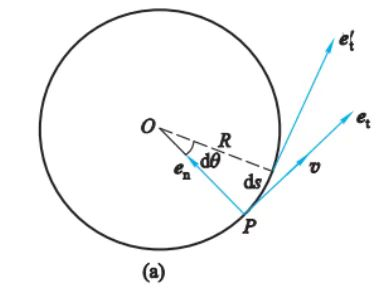
\includegraphics[width=0.3\linewidth]{images/naturesys.jpg}
	\caption{自然坐标系}
\end{figure}

\subsubsection{加速度}
\begin{figure}[h]
	\centering
	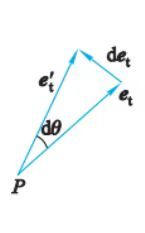
\includegraphics[width=0.25\linewidth]{images/nature.jpg}

\end{figure}

	{在极短时间内，$\mathbf{e}_t$与$\mathrm{d}\mathbf{e}_t$可视为相互垂直，则$\mathrm{d}\mathbf{e}_t$方向与$\mathbf{e}_n$相同,在大小上，$|\mathrm{d}\mathbf{e}_t|$=$|\mathrm{d}\theta|$。}
	
	$\mathbf{v}=v\mathbf{e}_t$
	
	\hspace*{\fill}
	
	$\mathbf{a}=\dfrac{\mathrm{d}\mathbf{v}}{\mathrm{d}t}=\dfrac{\mathrm{d}}{\mathrm{d}t}(v\mathbf{e}_t)=\dfrac{\mathrm{d}v}{\mathrm{d}t}\mathbf{e}_t+v\dfrac{\mathrm{d}\mathbf{e}_t}{\mathrm{d}t}$
	
	\vspace{12pt}
	
	$\mathrm{d}\mathbf{e}_t$=$\mathrm{d}\theta\mathbf{e} _n$
	
	\vspace{12pt}
	
	{对于$\frac{\mathrm{d}\mathbf{e}_t}{\mathrm{d}t}$：}

	$\dfrac{\mathrm{d}\mathbf{e}_t}{\mathrm{d}t}=\dfrac{\mathrm{d}\theta}{\mathrm{d}t}\mathbf{e}_n=\omega\mathbf{e} _n=\frac{v}{R}\mathbf{e} _n$
	
	{则$\mathbf{a}=\dfrac{\mathrm{d}\mathbf{v}}{\mathrm{d}t}\mathbf{e}_t+\dfrac{v^2}{R}\mathbf{e} _n$}
	
	{切向加速度$\mathbf{a}_t=\dfrac{\mathrm{d}\mathbf{v}}{\mathrm{d}t}\mathbf{e}_t$,表示速率变化快慢}
	
	{法向加速度$\mathbf{a}_n=\dfrac{v^2}{R}\mathbf{e} _n$，表示方向变化快慢}


\subsection{圆周运动的角量描述}

{角位置$\theta$}

{角位移$\Delta\theta$}

{角速度$\omega=\lim_{{\Delta}t\rightarrow0}\dfrac{\Delta\theta}{\Delta t}=\dfrac{\mathrm{d}\theta}{\mathrm{d}t}$}

{角加速度$\mathbf{a}=\lim_{{\Delta}t\rightarrow0}\dfrac{\Delta\omega}{\Delta t}=\dfrac{\mathrm{d}\omega}{\mathrm{d}t}=\dfrac{\mathrm{d}^2\theta}{\mathrm{d}t^2}$}

{匀变速圆周运动(类比匀加速直线运动)}

{$\omega=\omega_0 +\mathbf{a}t$}

{$\varphi=\varphi_0 +\omega_0 t+\frac{1}{2}\mathbf{a}t^2$}

{$\omega^2-{\omega_0}^2=2\mathbf{a}(\varphi-\varphi_0)$}


\subsection{角量和线量的关系}
\subsubsection{相关线量和角量}
以下是圆周运动中的相关线量和角量。

线量：速度$\mathbf{v}$、加速度$\mathbf{a}$

角量：角速度$\omega$、角加速度$\alpha$

\subsubsection{线量和角量的关系}
设圆的半径为$R$。

\begin{figure}[h]
	\centering
	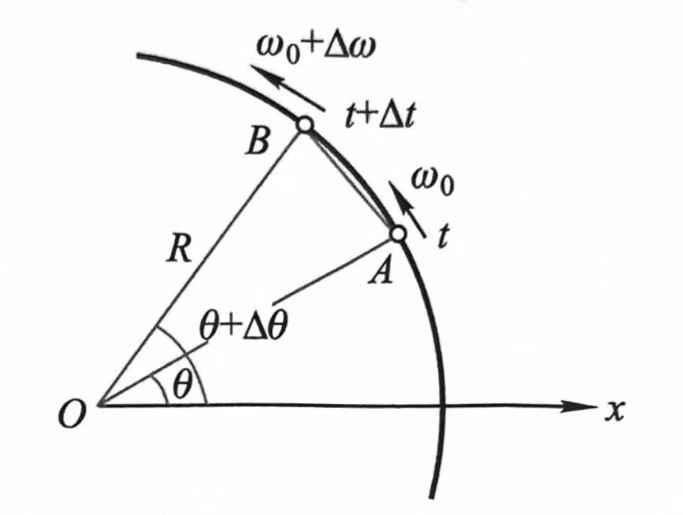
\includegraphics[width=0.5\textwidth]{images/ang-lin.jpg}
	\caption{线量和角量间的关系推导}
\end{figure}

\textbf{线速度和角速度：}
\begin{equation}
	v=R\omega
\end{equation}

\textbf{加速度和角加速度：}

切向加速度
\begin{equation}
	a_t=R\alpha
\end{equation}

法向加速度
\begin{equation}
	a_n=\frac{v^2}{R}=v\omega=R\omega ^2
\end{equation}

\subsubsection{一般平面曲线运动中的加速度}
质点沿轨迹作一般曲线运动时，上面讨论的有关变速圆周运动中加速度的结果也都是适用的。

但法向加速度式中的R要用曲线在该点处的曲率半径$\rho$来代替。

即
\begin{equation}
	\mathbf{a_t}=\frac{\mathrm{d}v}{\mathrm{d}t}\mathbf{e_t}
\end{equation}
\begin{equation}
	\mathbf{a_n}=\frac{v^2}{\rho}\mathbf{e_n}
\end{equation}
\begin{equation}
	\mathbf{a}=\mathbf{a_t}+\mathbf{a_n}=\frac{\mathrm{d}v}{\mathrm{d}t}\mathbf{e_t}+\frac{v^2}{\rho}\mathbf{e_n}
\end{equation}

法向加速度$a_n$处处指向曲率中心。 

一般来说，曲线上各点的曲率中心和曲率半径是逐点变化的。

\begin{figure}[h]
	\centering
	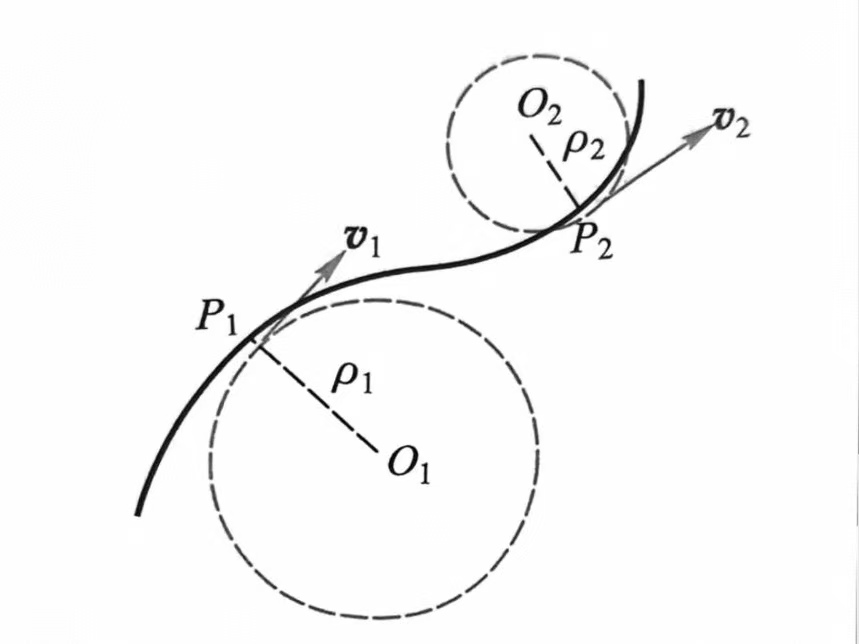
\includegraphics[width=0.5\textwidth]{images/rho.jpg}
	\caption{曲率圆和曲率半径}
\end{figure}

%
	\section{角量和线量的关系}
	\subsection{相关线量和角量}
	以下是圆周运动中的相关线量和角量。
	
	线量：速度$\mathbf{v}$、加速度$\mathbf{a}$
	
	角量：角速度$\omega$、角加速度$\alpha$
	
	\subsection{线量和角量的关系}
	设圆的半径为$R$。
	
	\begin{figure}[h]
		\centering
		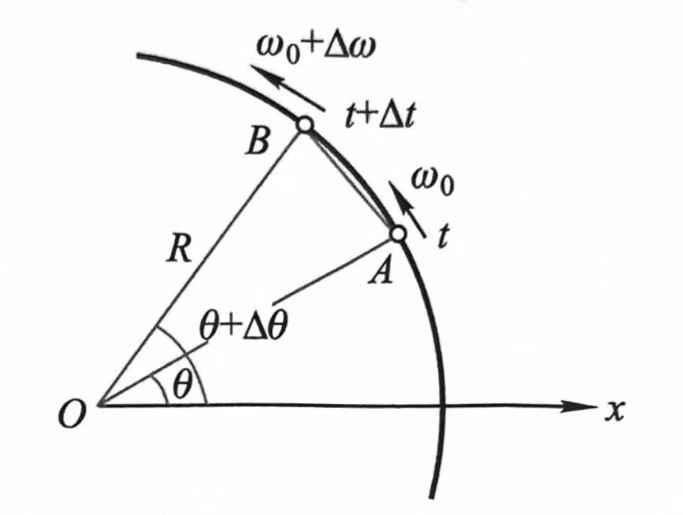
\includegraphics[width=0.5\textwidth]{images/ang-lin.jpg}
		\caption{线量和角量间的关系推导}
	\end{figure}
	
	\textbf{线速度和角速度：}
	\[
		v=R\omega
	\]
	
	\textbf{加速度和角加速度：}
	
	切向加速度
	\[
		a_t=R\alpha
	\]
	
	法向加速度
	\[
		a_n=\frac{v^2}{R}=v\omega=R\omega ^2
	\]
	
	\subsection{一般平面曲线运动中的加速度}
	质点沿轨迹作一般曲线运动时，上面讨论的有关变速圆周运动中加速度的结果也都是适用的。
	
	但法向加速度式中的R要用曲线在该点处的曲率半径$\rho$来代替。
	
	即
	\[
		\mathbf{a_t}=\frac{\mathrm{d}v}{\mathrm{d}t}\mathbf{e_t}
	\]
	\[
		\mathbf{a_n}=\frac{v^2}{\rho}\mathbf{e_n}
	\]
	\[
		\mathbf{a}=\mathbf{a_t}+\mathbf{a_n}=\frac{\mathrm{d}v}{\mathrm{d}t}\mathbf{e_t}+\frac{v^2}{\rho}\mathbf{e_n}
	\]
	
	法向加速度$a_n$处处指向曲率中心。 
	
	一般来说，曲线上各点的曲率中心和曲率半径是逐点变化的。
	
	\begin{figure}[h]
		\centering
		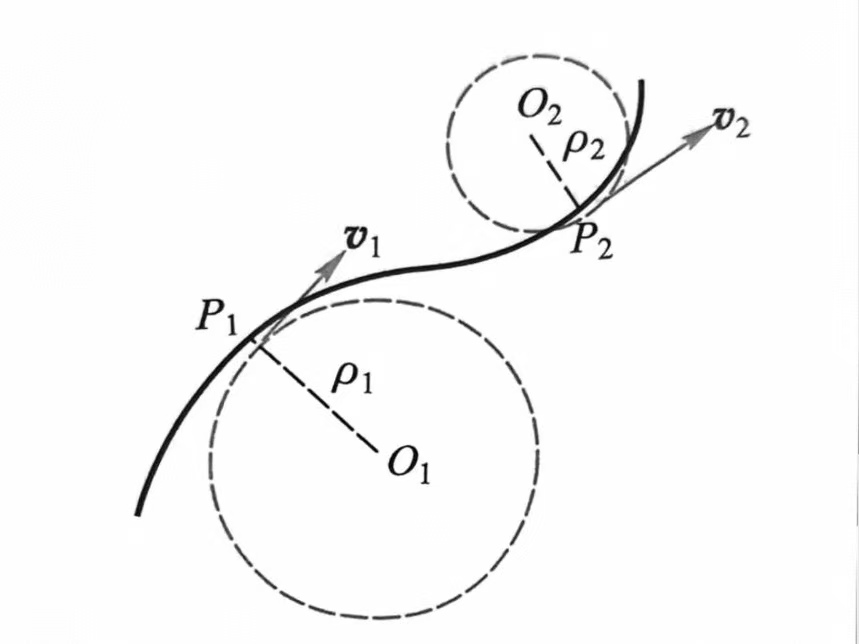
\includegraphics[width=0.5\textwidth]{images/rho.jpg}
		\caption{曲率圆和曲率半径}
	\end{figure}


%\include{sections/1.3}

	\section{相对运动}
	\subsection{使用前提}
	参考系$K$相对于参考系$K'$作\textbf{平动}。$K'$系的坐标原点$O'$相当于$K$系可作任意的直线或曲线运动，但它们的坐标轴的方向总是保持不变。

	\begin{figure}[h]
		\centering
		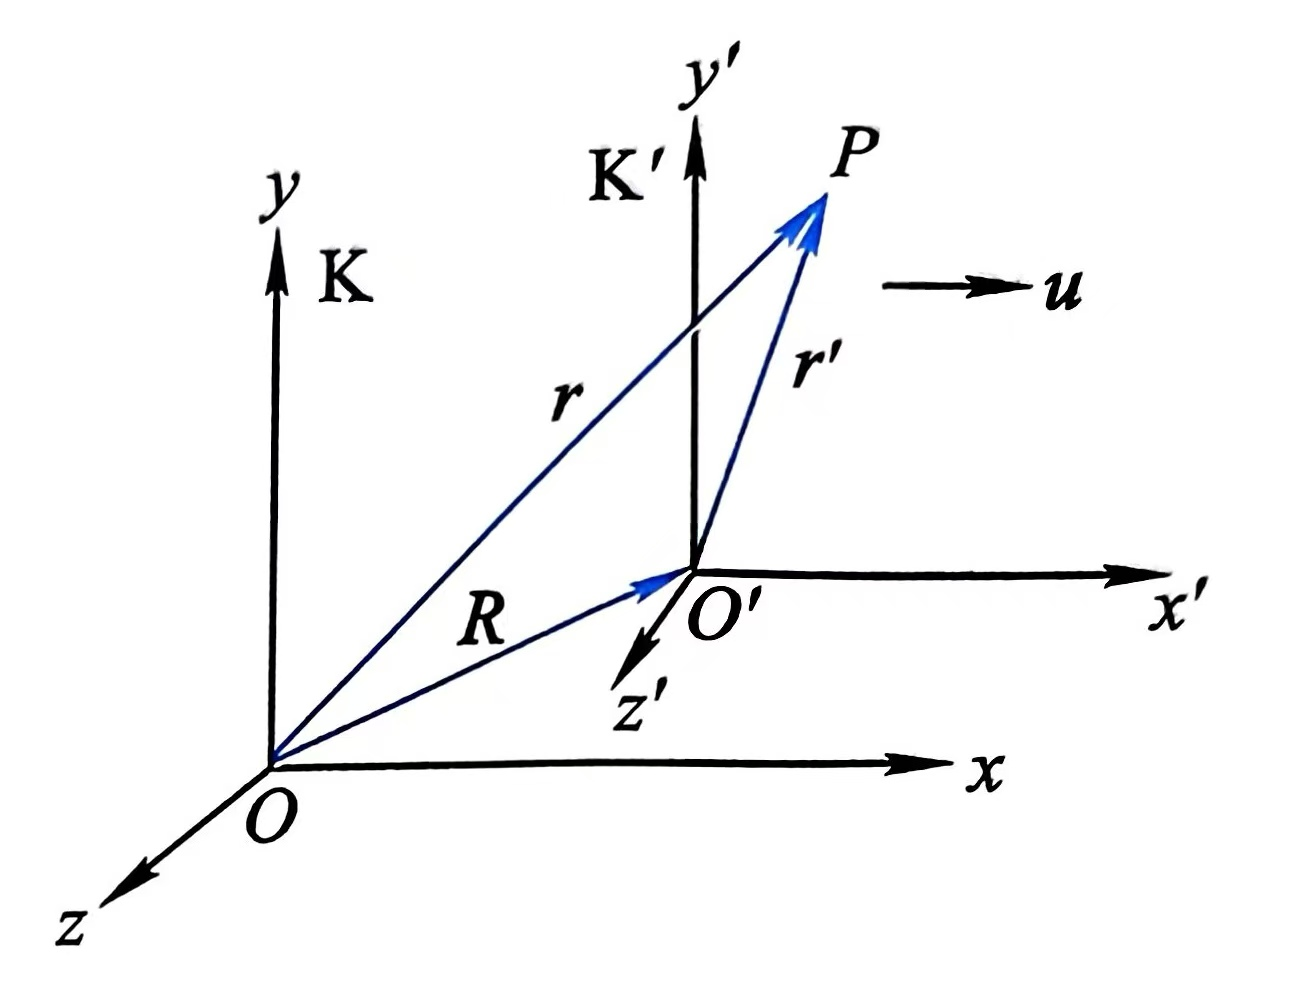
\includegraphics[width=0.5\textwidth]{images/revelate.jpg}
		\caption{相对运动关系图解}
	\end{figure}
	
	\subsection{重要公式}
	\subsubsection{位矢关系}
	
	$\vec{r}$：质点$P$在$K$系中的位矢。
	
	$\vec{r'}$：质点$P$在$K'$系中的位矢。
	
	$\vec{R}$：$K'$系原点$O'$对$K$系原点$O$的位矢。
		$$\vec{r}=\vec{r'}+\vec{R}$$
	
	\subsubsection{速度关系}
	
	绝对速度$\vec{v}$：质点相对于静止参考系$K$的速度。
	
	相对速度$\vec{v'}$：质点相对于运动参考系$K'$的速度。
	
	牵连速度$\vec{u}$：两参考系之间的相对速度。
		$$\vec{v}=\vec{v'}+\vec{u}$$
	
	\subsubsection{加速度关系}
	
	$\vec{a}$：质点相对于静止参考系$K$的加速度。
	
	$\vec{a'}$：质点相对于运动参考系$K'$的加速度。
	
	$\vec{a_0}$：两参考系之间的相对加速度。
	
		$$\vec{a}=\vec{a'}+\vec{a_0}$$
	
	特别地，若$\vec{a_0}=0$，则$\vec{a}=\vec{a'}$。表明质点在两个相对作匀速直线运动的参考系中的加速度是相等的。质点的加速度相对于作匀速直线运动的各个参考系是个绝对量。
	

	\section{动力学————牛顿运动定律}
	\subsection{牛顿运动定律}
	
	
	
	{\footnotesize 物理学史：牛顿（ I . Newton ）《自然哲学的数学原理》出版标志着经典力学体系的确立。}
	
	
	动力学是研究物体与物体之间的相互作用以及由于这种相互作用而引起的物体运动状态的变化规律，其基础是牛顿三大定律。
	\begin{theorem}[牛顿第一定律]
		任何物体都保持静止或沿一直线作匀速运动的状态，直到作用在它上面的力迫使它改变这种状态为止。
	\end{theorem}
	\begin{note}
	 	第一定律建立了惯性和力的确切概念。任何物体都具有惯性，因此第一定律又被叫做惯性定律( law of inertia )。惯性( inertia )：物体所具有的保持其原有运动状态不变的特性。
	
	牛顿第一定律动力学是研究物体之间的相互作用以及由于这种相互作用而引起的平动物体或质点运动状态的变化规律，也是其他定律的基础。
	
	惯性分类：质点运动的平动惯性，转动的转动惯性，热运动的热惯性，电磁运动的电磁惯性。
	
	牛顿第一定律对惯性参考系( inertial frame )都适用，即一个不受力作用的物体将保持其静止或匀速直线运动的状态不变。不遵守牛顿第一定律的参考系，称为非惯性参考系，简称非惯性系。
	\end{note}
	\begin{theorem}[牛顿第二定律]
		
		物体受到外力作用时，加速度的大小与外力的大小成正比，并与物体的质量成反比，加速度的方向与外力的方向相同。
	
\centering	$ \vec{F=ma } $
	
	单位：$kg ，m /s^2，N$ 
	
	动量( momentum )，用 $p$ 表示，即\\
	
	$ p=mv $
	
	第二定律实质上是\\
	
	$ \frac{dp}{dt}= F  $
	
	
	
	$ F=m\frac{d^{2}r}{dt^{2}} $
	
	称为质点的动力学方程。\\
	\end{theorem}

	\begin{note}
	牛顿第二定律注意：
	
	(1)瞬时性，第二定律定量地表述了物体的加速度与所受外力之间的瞬时关系，它们同时存在，同时改变，同时消失。
	
	(2)矢量性，力和加速度的叠加和作用效果遵从矢量三角形法则。
	
	(3)对应性，一个力对应一个加速度.
	\end{note}
	
	\begin{definition}[牛顿第三定律]两个物体之间的作用力和反作用力，在同一直线上，大小相等方向相反。


即
$ F_{ A B } = - F_{ B A }  $

若把
$F _ { AB } \text{和} F _ { BA }$中的一个叫做作用力（acting force），则另一个就叫反作用力（reacting force）。

第三定律揭示了力的特性：成对性，一致性，同时性。
\end{definition}
\subsection{力学中的常见力}

力学中常见力有万有引力、重力、弹性力、摩擦力等。

\begin{definition}[万有引力]
	
	
	牛顿万有引力定律（law of universal gravity）:质量分别为m1和m2的两个质点，相距为r时，引力为
	$ F = G \frac { m _ { 1 } m _ { 2 } } { r ^ { 2 } } $
	
	式中G叫做引力常量（gravitational constant），2018年国际推荐值为
	$ G = 6 . 6 7 4 3 0 \times 1 0 ^ { - 1 1 } N \cdot m ^ { 2 } / k g ^ { 2 } $
\end{definition}

式中的质量反映了物体的引力性质，叫做引力质量（gravitational mass），和反映物体惯性的惯性质量在意义上是不同的。

适用范围：两个质点，均匀质量球体。


\begin{definition}[重力]因地球吸引而使物体受到的力。\end{definition}


重力的方向，重力加速度的方向：竖直向下的．\\[0.01cm]

{\small	由于地球的自转效应，地球不是一个惯性系。从某个惯性系（如日心系）看来，地球上的物体将随地球绕地轴作圆周运动。物体所受地球的引力有一部分提供了向心力，剩余的分力才是重力重力的大小。
	
	重力探矿法:地球内某处存在大型矿藏，破坏了地球质量的对称分布，使该处的重力加速度值表现出异常，因此可通过重力加速度的测定来探矿。}\\[0.01cm]



\begin{definition}[弹力](elastic force):发生形变的物体，由于要恢复原状，对与它接触的物体会产生力的作用,简称弹力。
\end{definition}

弹力的主要三种表现形式：

(1)正压力：

正压力( normal pressure )或支持力( support force )：两个物体通过一定面积相互挤压。

{\small	如，屋架压在柱子上，重物放在桌面上。大小:挤压程度。方向:垂直于接触面而指向对方。}\\

(2)绳中的张力：

张力( tension )：把绳分为两部分，这种内部的两部分绳的相互拉力。

当绳没有加速度，或质量可以忽略时，绳上各点的张力都是相等的，而且就等于外力条件。\\

(3)弹簧的弹力：

弹力（恢复力）：当弹簧被拉伸或压缩时，它就会对与之相连的物体有弹力作用。在弹性限度内，其大小和形变成正比．以 F 表示弹力，以 x 表示形变亦即弹簧的长度变化，则

$	F =- kx  $

式中 k 叫做弹簧的劲度系数（ stiffness ），负号表示弹力的方向总是和弹簧位移的方向相反，弹力总是指向要恢复它原长的方向。\\

4.摩擦力

摩擦力( friction force ):两个相互接触的物体在沿接触面相对运动时，或者有相对运动的趋势时，在接触面之间产生一对阻碍相对运动的力。\\

(1)静摩擦力( static friction force):相互接触的两个物体在外力作用下，虽有相对运动的趋势，但并不产生相对运动。\\

每个物体所受静摩擦力的方向与该物体相对于另一物体的运动趋势方向相反。静摩擦力的大小视外力的大小而定，介乎0和最大静摩擦力 F 之间。最大静摩擦力正比于正压力 F ，即\\

$	F_{s}=\mu_{s} F_{N}   $

静摩擦因数$\mu_{s}$( static friction factor )，与接触面的材料和表面情况有关。\\

(2)动摩擦力( dynamic friction force ):当外力超过最大静摩擦力时，物体间将会产生相对运动的摩擦力。\\

动摩擦力 F 也与正压力 F 成正比，\\

$	F_{k} = \mu_{k} F_{N}  $
动摩擦因数$\mu_{k}$( dynamic friction factor )和相互接触的两物体的材料，表面情况，物体的相对速度有关。在大多数情况下，它随速度的增大而减小。\\

对于给定的一对接触面来说， $\mu_{s}> \mu_{k}$。\\

(3)湿摩擦力:固体在流体中运动时，沿着接触面出现的摩擦力。\\

1：在固体与流体相对运动速率不大时\\
$	F_{d} = -kv $

2：在固体与流体相对运动速率较大时\\
$	F_{d} =-kv\overrightarrow{v} $

湿摩擦力远小于干摩擦力！
\subsection{基本相互作用}	
自然界物体之间的相互作用力，可归结为四种相互作用：\\

引力相互作用:物体之间相互吸引的作用，这种力存在于一切物体之间，其强度随距离的增大而减弱。


电磁相互作用:电荷之间的相互作用，包括同种电荷之间的排斥和异种电荷之间的吸引，以及磁体之间的相互作用。


强相互作用:原子核内部将质子粘结在一起的力，仅在原子核内部起作用，外部没有任何表现。


弱相互作用:基本粒子之间的一种特殊作用，其强度比强相互作用和电磁作用都弱，作用范围也比强相互作用更小。



\section{非惯性系和惯性力}

\begin{definition}[非惯性系]
    惯性系：相对一个惯性系作匀速直线运动的一切参考系。\\
    非惯性系:相对地面参考系（惯性系）作加速运动的参考系。\\
\end{definition}


\begin{example}[非惯性系理解]
    以加速启动的列车为参考系，在列车车厢内的人看到小车的情况就大不一样，小车是向
    列车车尾方向作加速运动的．小车受力的情况没有变化，合力仍然是0，却有了加速度，
    这是违反牛顿运动定律的．因此，加速运动的列车是个非惯性系，相对于它，牛顿运动
    定律不再成立．
\end{example}


\begin{definition}[惯性力]
    设有一质点，质量为$m$ ，所受的合外力为 $\vec{F}$ ，它相对于惯性系的加速度为 a ，根
据牛顿第二定律，有\\
\centering$\vec{F} = m\vec{a}$\\
设想另一参考系，相对于惯性系以加速度 $\vec{a}$ 。作直线运动，在此参考系中，质点的加速度为 $\vec{a'}$，
由运动的相对性,可知\\
 $\vec{a = a '+a_0}$\\
将此式代人牛顿运动定律可得\\
 $\vec{F = m ( a '+ a)= ma '+ ma}$\\
将上式改写成\\
 $\vec{F +(- ma_0 )= ma '}$\\
此式说明，在非惯性系观察物体运动时，除了实际的外力之外，物体还受到一个大小和方向由$﹣ m\vec{a}$ 。
表示的力．这个力称为惯性力．这样就可以形式上应用牛顿第二定律去分析问题．
\par
在直线加速的非惯性系中，质点$m$受到的惯性力$\vec{F_惯}$：\\
$\vec{F_惯}=-m\vec{a_0}$\\


\begin{note}
    \textcolor{red}{\kaishu 公式中负号为与加速度$\vec{a_0}$方向相反.$\vec{a_0}$为系统加速度.}
\end{note}


在匀速转动的参考系中，质点$m$受到的惯性力$\vec{F_惯}$：\\
$\vec{F_惯}=-mw^2r\vec{e_r}$\\
因此：若质点静止在匀速转动的参考系中：\\
$\sum \vec{F_外}+\vec{F_惯}=\vec{0}$ \\


\begin{note}
    \textcolor{red}{\kaishu 此力称为惯性离心力.}
\end{note}


\par
\par


\begin{supplement}[科里奥利加速度]
    \textcolor{blue}{\kaishu 物体在做牵连运动的同时,沿旋转半径做相对运动,由牵连运动和相对运动交互
    耦合而形成的加速度称为科里奥利加速度.\\}
    \centering$\vec{F_科}=2m\vec{v}\times\vec{\omega } $\\
    \begin{note}
        \textcolor{red}{\kaishu 1、该公式中角速度$\vec{\omega }$为矢量，方向可由右手螺旋定则确定.\\
        2、公式中$\vec{v}$为物体相对匀速转动非惯性系的相对速度.}
    \end{note}

\end{supplement}

\end{definition}



\chapter{守恒定律}
\section{质心运动定理}
\begin{definition}[质心]
    质心是与质点系质量分布有关的一个代表点，它的位置在平均意义上代表着质量分布的中心。质心的位置即为位矢关于质量的加权平均。

    \[
        \boldsymbol{r}_c =\dfrac{\sum m_i\boldsymbol{r}_i }{m}
    \]

    对于质量连续的物体，表达式变为：

    \[
        \boldsymbol{r}_c =\dfrac{\int \boldsymbol{r}_i \mathrm{d}m}{m}
    \]
    
\end{definition}
\label{def:mass-center}
\begin{attention}{ }{2.1.1}
    重心和质心是两个不同的概念！

    只有当物体所在区域重力加速度分布均匀时，重心和质心在几何上重合。

\end{attention}

由定义\ref{def:mass-center}，质心的速度为
\[
    \boldsymbol{v}_c=\dfrac{\mathrm{d}\boldsymbol{r}_c}{\mathrm{d}t}=\dfrac{\sum m_i\dfrac{\mathrm{d}\boldsymbol{r}_i}{\mathrm{d}t}}{\sum m_i}=\dfrac{\sum m_i\boldsymbol{v}_i}{\sum m_i}
\]
同理，质心的加速度为
\[
    \boldsymbol{a}_c=\dfrac{\sum m_i\boldsymbol{a}_i}{\sum m_i}
\]

根据牛顿第二定律，质点系中各个质点的运动方程为
$$m_{1}\boldsymbol{a}_{1}=m_{1}\:\frac{\mathrm{d}\boldsymbol{v}_{1}}{\mathrm{d}t}=\boldsymbol{F}_{1}+\boldsymbol{F}_{12}+\boldsymbol{F}_{13}+\cdots+\boldsymbol{F}_{1n}$$


$$m_{2}\boldsymbol{a}_{2}=m_{2}\frac{dv_{2}}{dt}=\boldsymbol{F}_{2}+\boldsymbol{F}_{21}+\boldsymbol{F}_{23}+\cdots+\boldsymbol{F}_{2n}$$
$$\vdots$$
$$m_{n}\boldsymbol{a}_{n}=m_{n}\frac{dv_{n}}{dt}=\boldsymbol{F}_{n}+\boldsymbol{F}_{n1}+\boldsymbol{F}_{n2}+\cdots+\boldsymbol{F}_{n\:n-1}$$


在上述各式中，$\boldsymbol{F}_1,\boldsymbol{F}_2,\cdotp\cdotp\cdotp,\boldsymbol{F}_n$表示质点系外的物体对各个质点的作用力，即为质点系所受的外力；而 $\boldsymbol{F}_{12},F_{21},\cdots,\boldsymbol{F}_{in},\boldsymbol{F}_{ni},\cdots$表示质点系内各个质点之间的相互作用力，这些力即为质点系的内力.根据牛顿第三定律，内力在质点系内总是成对地出 现 的 , 它 们 之 间 满 足 关 系 式 $\boldsymbol{F}_{12}+ \boldsymbol{F}_{21}= 0, \cdots , \boldsymbol{F}_{in}+ \boldsymbol{F}_{ni}= 0, \cdots .$因 此 , 把 上 述 各 式 相 加

$$m_{1}\boldsymbol{a}_{1}+m_{2}\boldsymbol{a}_{2}+\cdots+m_{n}\boldsymbol{a}_{n}=\boldsymbol{F}_{1}+\boldsymbol{F}_{2}+\cdots+\boldsymbol{F}_{n}$$

或者写成

$$\sum m_i\boldsymbol{a}_i=\sum\boldsymbol{F}_i$$

由此，可以得到以下结论：
\begin{theorem}[质心运动定理]
    \[
    \sum \boldsymbol{F}_i=m\boldsymbol{a}_c
    \]
\end{theorem}

\begin{knowledge}{ }{2.1.2}

    在多体系统中，研究质心的运动规律以及使用质心参考系可以大大简化研究的复杂性，也有二体修正等方法以及结论可帮助研究相应的物理过程，有兴趣的读者可自行探索。

\end{knowledge}


\section{动量守恒定律}
\subsection{动量定理}
\begin{definition}[冲量]
    我们把作用在物体上的力的时间累积效应称为冲量，常用$I$来表示，对于物体上的合力$F$，根据牛顿第二定律，有：

    \[
        F = ma = m\dfrac{\mathrm{d}v}{\mathrm{d}t}= \dfrac{\mathrm{d}mv}{\mathrm{d}t} = \dfrac{\mathrm{d}p}{\mathrm{d}t}
    \]

    分离变量得
    
    \[
       F\mathrm{d}t=\mathrm{d}(mv)
    \]

    其中$F\mathrm{d}t$被称为力$F$的元冲量，对时间积分得

    \[
        I=\int_{\boldsymbol{t}_1}^{\boldsymbol{t}_2}F\mathrm{d}t=m\Delta v=m\boldsymbol{v}_2-m\boldsymbol{v}_1=\boldsymbol{p}_2-\boldsymbol{p}_1
    \]

    其中$\int_{\boldsymbol{t}_1}^{\boldsymbol{t}_2}F\mathrm{d}t$是变力$F$在时间$\boldsymbol{t}_2-\boldsymbol{t}_1$内所有元冲量的矢量合
    ，上述式子说明质点在运动过程中所受合外力的冲量等于该物体动量的增量，
    这个结论叫做质点的动量定理。

   

\end{definition}
\label{def:theorem of momentum}
\begin{attention}{ }{2.2.1}
    （1）不管物体在运动过程中动量变化的细节如何，合力冲量的大小和方向总等于物体初末动量的矢量差

    （2）动量定理为矢量方程，应用时可直接矢量作图，也可在平面直角坐标系中写成投影式

    （3）对于作用时间短促而变化极大的力（冲力），可用动量定理求冲力平均值

    （4）动量定理可以用于解决变质量问题

    （5）动量定理对于所有惯性系适用

\end{attention}


\subsection{质点系动量定理}
对于一拥有n个质点的质点系：

根据动量定理，质点系中各个质点的动量定理方程为
$$\mathrm{d}\boldsymbol{p}_{1}=(\boldsymbol{F}_{1}+\boldsymbol{F}_{12}+\boldsymbol{F}_{13}+\cdots+\boldsymbol{F}_{1n})\mathrm{d}t$$


$$\mathrm{d}\boldsymbol{p}_{2}=(\boldsymbol{F}_{2}+\boldsymbol{F}_{21}+\boldsymbol{F}_{23}+\cdots+\boldsymbol{F}_{2n})\mathrm{d}t$$
$$\vdots$$
$$\mathrm{d}\boldsymbol{p}_{n}=(\boldsymbol{F}_{1}+\boldsymbol{F}_{n1}+\boldsymbol{F}_{n2}+\cdots+\boldsymbol{F}_{n n-1})\mathrm{d}t$$


在上述各式中，$\boldsymbol{F}_1,\boldsymbol{F}_2,\cdotp\cdotp\cdotp,\boldsymbol{F}_n$表示质点系外的物体对各个质点的作用力，即为质点系所受的外力；而 $\boldsymbol{F}_{12},F_{21},\cdots,\boldsymbol{F}_{in},\boldsymbol{F}_{ni},\cdots$表示质点系内各个质点之间的相互作用力，这些力即为质点系的内力.根据牛顿第三定律，内力在质点系内总是成对地出 现 的 , 它 们 之 间 满 足 关 系 式 $\boldsymbol{F}_{12}+ \boldsymbol{F}_{21}= 0, \cdots , \boldsymbol{F}_{in}+ \boldsymbol{F}_{ni}= 0, \cdots .$因 此 , 把 上 述 各 式 相 加

$$\mathrm{d}\boldsymbol{p}_{1}+\mathrm{d}\boldsymbol{p}_{2}+\cdots+\mathrm{d}\boldsymbol{p}_{n}=(\boldsymbol{F}_{1}+\boldsymbol{F}_{2}+\cdots+\boldsymbol{F}_{n})\mathrm{d}t$$

或者写成

$$\sum \mathrm{d}\boldsymbol{p}_i=\sum\boldsymbol{F}_i\mathrm{d}t$$

对时间积分，可以得到以下结论：
\begin{theorem}[质点系动量定理]
    \[
    \sum \int_{\boldsymbol{t}_1}^{\boldsymbol{t}_2}\boldsymbol{F}_i\mathrm{d}t=\sum \boldsymbol{m}_i\boldsymbol{v}_{2i} - \sum \boldsymbol{m}_i\boldsymbol{v}_{1i}
    \]
    上述式子表示：在某段时间内，作用在质点上的所有外力在同一时间内的冲量的矢量和等于质点系总动量的增量。
\end{theorem}


\subsection{动量守恒定律}

    对于系统来说，若所受合外力的矢量和为0（$\sum\boldsymbol{F}_i=0$）,有质点系动量定理得
$$
(\sum \boldsymbol{m}_i\boldsymbol{v}_{i})\mathrm{d}t=0
$$
积分得
$$
\sum \boldsymbol{m}_i\boldsymbol{v}_{i}=C(\sum\boldsymbol{F}_i=0)
$$
其中C为一常矢量

上述式子说明：如果系统所受到的外力矢量和为零（即$\sum\boldsymbol{F}_i=0$）时，系统的总动量保持不变

\begin{knowledge}{ }{2.2.2}

    （1）运用动量守恒定理前首先要分析系统内各物体所受外力，在1.合外力为零2.较短时间内外力相较于内力可忽略不计等情况下可以使用

    （2）动量守恒定律的数学表达式是一个矢量式，在实际计算中，可使用它按个坐标轴分解的分量式

    有时，系统的外力之和并不为0，但外力在某一方向上的分量之和却为0，此时，尽管系统总动量不守恒，但总动量在该方向上的分量守恒

    （3）所有质点的动量都必须是对同一参考系的

\end{knowledge}


\section{质点的角动量定理和角动量守恒定律}
\subsection{基本概念}
定义：质点对某一给定点$O$的位矢$\vec{r}$与质点动量$\vec{p}$的矢积为质点对给定点的角动量。
$$\vec{L}=\vec{r}\times \vec{p}$$

大小：$L=pr\sin{\varphi}$

方向：垂直于位矢$\vec{r}$和动量$\vec{p}$所组成的平面。指向$\vec{r}$经小于$180^{\circ}$的角转到$\vec{p}$的右手螺旋前进的方向。
	\begin{figure}[h]
	\centering
	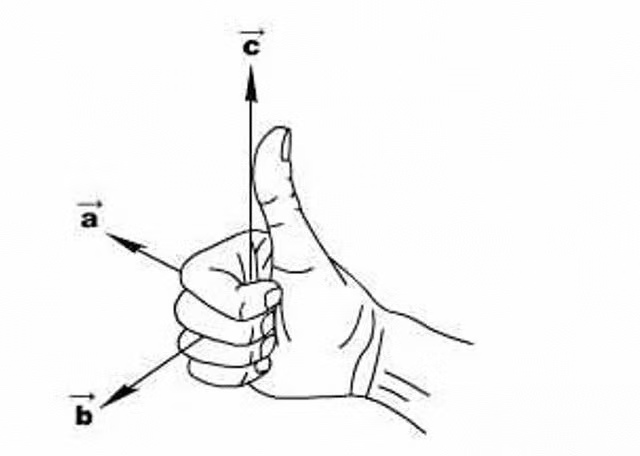
\includegraphics[width=0.5\textwidth]{images/cross.jpg}
	\caption{叉乘的右手定则}
   \end{figure}

单位：$kg\cdot m^2/s$

标矢性：矢量

意义：描述物体的转动特征。

\subsection{引起变化的因素}
\subsubsection{质点的角动量定理}
内容：质点对给定点的角动量随时间的变化率等于作用于质点的合力对该点的力矩。

推导：$$\frac{\mathbf{d}\vec{L}}{\mathbf{d}t}=\frac{\mathbf{d}(\vec{r}\times\vec{p})}{\mathbf{d}t}=\frac{\mathbf{d}\vec{r}}{\mathbf{d}t}\times\vec{p}+\vec{r}\times\frac{\mathbf{d}\vec{p}}{\mathbf{d}t}=\vec{r}\times\frac{\mathbf{d}\vec{p}}{\mathbf{d}t}=\vec{r}\times\vec{F}$$

注意：使用定理时，力矩中的位矢$\vec{r}$和角动量中的位矢$\vec{r}$应相对同一给定点$O$。

\subsubsection{力矩}
定义：力的作用点相对给定点的位矢$\vec{r}$与力$\vec{F}$的矢积为力对给定点的力矩。

单位：$N\cdot m$（牛顿米）

标矢性：矢量

[辨别]力矩与功：$\sin\varphi\text{与}\cos\varphi$、$\vec{r}$与$\mathbf{d}\vec{r}$、矢量与标量

\subsection{质点的角动量守恒定律}
内容：如果作用在质点上的合力对某给定点$O$的力矩为零，则质点对该点的角动量在运动过程中保持不变。

经典场景：质点在有心力作用下运动，角动量守恒。

[例]圆周运动、行星在公转轨道上运动……

\subsection{推广：质点系}
\subsubsection{质点系的角动量定理}
内容：质点系对给定点的角动量随时间的变化率等于外力对该点力矩的矢量和。将$\sum\vec{M_{i\text{外}}}$简写为$\vec{M}$，得
$$\vec{M}=\frac{\mathbf{d}\vec{L}}{\mathbf{d}t}$$

外力与内力：由牛顿第三定律可知，成对出现的内力对给定点的力矩矢量和为零
（类似于冲量，区别于功）。

\subsubsection{质点系的角动量守恒定律}
内容：如果$M=0$，得
$$\vec{L}=\text{常矢量}$$



\section{功~动能~动能定理}

\subsection{功的相关概念}

\subsubsection{机械功}

\textbf{力和物体在力的方向上移动距离的乘积，叫做力对物体做的功。}

	$$\mathrm{d}A=\mathbf{F}\cdotp\mathrm{d}\mathbf{r}=|\mathbf{F}| |\mathrm{d}\mathbf{r}|\cos\theta=F\mathrm{d}s\cos\theta$$
	
	$$ A=\int\mathrm{d}A=\int_{a}^{b}\mathbf{F}\cdotp\mathrm{d}\mathbf{r}=\int_{a}^{b} F\cos\theta\mathrm{d}s$$
	
关于概念，辨析以下几点：

1.力在时间上的累积作用是动量，力在空间上的累积作用是功。

2.功是标量，无方向，正负代表做功的正负，单位为J或$N\cdotp m$。

3.$\mathbf{F}$是恒力，对于变力，在一段极小的位移中仍可视作恒力。

4.由于力是矢量，可以在$x,y,z$轴进行分解，因此功也可以在$x,y,z$轴分解，总功等于三者的代数和。

\subsubsection{功率}

\textbf{力在单位时间内做的功，叫做功率。}
$$P=\dfrac{\mathrm{d}A}{\mathrm{d}t}=\dfrac{\mathbf{F}\cdotp\mathrm{d}\mathbf{r}}{\mathrm{d}t}=\mathbf{F}\cdotp\mathbf{v}$$

1.功率表示力的做功快慢程度。

2.功率的单位为W或$J/s$。

\subsection{能量}

\textbf{能量是物体状态的单值函数，是各种运动状态的一般量度。}

机械运动状态由位置和速率描述，因此位置和速率是机械运动的状态参量，位置决定势能，速率决定动能，机械能由动能和势能组成。

\subsection{动能定理}

$$\mathrm{d}A=\mathbf{F}\cdotp\mathrm{d}\mathbf{r}=F\cos\theta|\mathrm{d}r| $$
由牛顿第二定律，$$F\cos\theta=m\mathbf{a}_t=m\dfrac{\mathrm{d}\mathbf{v}}{\mathrm{d}t} $$
得到$$\mathrm{d}A=F\cos\theta|\mathrm{d}r|=m\dfrac{\mathrm{d}\mathbf{v}}{\mathrm{d}t}\mathbf{v}\mathrm{d}t=m\mathbf{v}\mathrm{d}\mathbf{v} $$
因此，$$A=\int_{\mathbf{v}_a}^{\mathbf{v}_b} m\mathbf{v}\mathrm{d}\mathbf{v}=\frac{1}{2}m{\mathbf{v}_b}^2-\frac{1}{2}m{\mathbf{v}_a}^2$$
$$A=E_{kb}-E_{ka}$$

1.动能定理连接起了功与能之间的关系，将过程量与状态量相联系，\textbf{合外力对质点做的功等于质点动量的增量}。

2.由于运用了牛顿第二定律，因此动能定理只能在惯性系下成立，但在不同的惯性参考系中，动能定理形式上保持不变，即形式上与参考系的选择无关。

	\section{ 保守力 成对力的功 势能}
	
	\subsection{保守力}
	
\begin{definition}[保守力]
	功的大小只与物体初末位置有关，与路径无关。\
\end{definition}
	特性：质点沿任意闭合路径运动一周，做功为零。
	
	 
		\begin{example}
			重力（场中的力），弹力，万有引力（引力场）。非保守力：摩擦力等。
		\end{example}
	
	\subsection{成对力的功}
	
	成对保守力的功只取决于质点相对位移的变化。
	
	\subsection{势能}
	
	势能存在于不同物体之间，属于系统所具有的能量形式。
	
	势能差具有绝对意义，系统势能量值只有相对意义。
	
\begin{definition}[势能曲线]
	保守力沿某坐标轴的分量等于势能对此坐标轴的导数的负值。
\end{definition}
	
	
\subsubsection{用处：1.由曲线求保守力。}
	$F_{c}(x)=-\frac{\partial E_{p}}{\partial x}$
	\subsubsection{2.确定质点运动范围。}
	{ 带入极端情况，如0等求解。}
	\subsubsection{3.确定平衡位置，判断平衡稳定性。}
	
	\section{质点系的功能原理，机械能守恒定律}


	\begin{theorem}[质点系的动能原理]
		单个质点动能定理推广到多个物体：\\
		对于一个由二质点组成的系统$m_1,m_2$：\\
		质点$m_1$受到的外力为$\overrightarrow{ F_1}$，质点$m_2$受到的外力为$\overrightarrow{ F_2}$.\\
		两质点相互作用力分别为$\overrightarrow{F_{21}}, \overrightarrow{F_{12}}$\\
		在这些作用力下，质点$1,2$各自的路径为$s_1,s_2$.\\
		则对质点一运用动能定理有:\\
		\centering$\int \overrightarrow{F_1} \cdot  {d }\overrightarrow{r_1}+\int \overrightarrow{F_{21}} \cdot  {d }\overrightarrow{r_1}=\Delta E_{k1} $\\
		同样对于质点 $2$有：\\
		$\int \overrightarrow{F_2} \cdot  {d }\overrightarrow{r_2}+\int \overrightarrow{F_{12}} \cdot  {d }\overrightarrow{r_2}=\Delta E_{k2} $\\
		两式相加，即有：\\
		$\int \overrightarrow{F_1} \cdot  {d }\overrightarrow{r_1}+\int \overrightarrow{F_{21}} \cdot  {d }\overrightarrow{r_1}+\int \overrightarrow{F_2} \cdot  {d }\overrightarrow{r_2}+\int \overrightarrow{F_{12}} \cdot  {d }\overrightarrow{r_2}=\Delta E_k'+\Delta E_k" $\\
		外力做功用$A_e$表示，内力做功用$A_i$表示：\\
		则质点系动能定理可以表示为：\\
		$A_e+A_i=\Delta E_k$\\
		\textcolor{blue}{\kaishu 即系统的内力和外力做功的总和等于系统动能的增量。}\\
	\end{theorem}
	
	\begin{center}
		
	\begin{tikzpicture}[
		dot/.style={circle,fill,inner sep=1pt},
		arrow/.style={->,>=latex},
		% 加载 calc 库
		remember picture, 
		every node/.style={remember picture}
	]
		% 质点 1
		\node[dot,label={[label distance=0.2cm]below:$m_1$}] (m1) at (8,1) {};
	
		% 质点 2
		\node[dot,label={[label distance=0.2cm]below:$m_2$}] (m2) at (14,1) {};
	
		\draw[dashed] (5,0) rectangle (17,2);
		% 绘制力 F2（箭头从 m2 的左侧偏移到 m1 的右侧偏移）
		\draw[arrow] ($(m2) - (0.5,0)$) -- ($(m1) + (4,0)$) node[midway,above] {$\overrightarrow{F_{21}}$};
		\draw[arrow] ($(m1) + (0.5,0)$) -- ($(m2) - (4,0)$) node[midway,above] {$\overrightarrow{F_{12}}$};
		\draw[arrow] ($(m1) - (0.5,0)$) -- ($(m1) - (1.5,-0.5)$) node[midway,above] {$\overrightarrow{F_{1}}$};
		\draw[arrow] ($(m2) + (0.5,0)$) -- ($(m2) + (1.5,-0.5)$) node[midway,above] {$\overrightarrow{F_{2}}$};
	\end{tikzpicture}
	
	\end{center}
	
	\begin{theorem}[质点系的功能原理]
		对于系统的内力来说，具有保守力和非保守力之分。因此，内力做功可以分为保守力做功$A_{ie}$,非保守力做功为$A_{id}$.\\
		\centering$A_i = A_{ie} + A_{id}$\\
		保守力做功$A_{ie}$等于系统势能增量的负值表示：\\
		$A_{ie} = -\Delta E_p$\\
		则有：\\
		$A_{e} + A_{id}=\Delta E_k + \Delta E_p = \Delta E$\\
		\textcolor{blue}{\kaishu 即系统机械能的增量等于外力做功与非保守内力做功的总和。}
	\end{theorem}
	
	
	\begin{theorem}[机械能守恒定律]
		\textcolor{blue}{\kaishu 如果一个系统只有保守力做功，其他内力和一切外力都不做功，则系统内个物体的动
		能和势能可以互相转化，但机械能总值不变。}
	\end{theorem}
	
	
	\begin{definition}[孤立系统]
		不受外界作用的系统。
	\end{definition}
	
	
	\begin{theorem}[能量守恒定律]
		一个孤立系统经历任何变化，该系统的所有能量的总和是不变的，能量只能从一种形式转化为另一种形式，或从系统
		内一个物体传给另一个物体。
	\end{theorem}
	  
	\par
	\begin{exercise}[宇宙速度]
		讨论三种宇宙速度。\\
	\begin{center}
			
		\begin{tikzpicture}[scale=1.5]
			% 绘制地球（填充蓝色）
			\shade[ball color=blue!50] (0,0) circle (0.5cm);
			
			% 第一宇宙速度：圆形轨道（红色虚线）
			\draw[red, dashed] (0,0) circle (1cm);
			\node[red, above] at (0,1) {$v_1$（圆轨道）};
			
			% 第二宇宙速度：抛物线轨道（蓝色，与圆相切于右侧）
			\draw[blue, thick, domain=0:2.5, samples=100] 
				plot ({-1 + 0.3*\x^2}, {0.6*\x}) 
				node[left] {$v_2$（抛物线）};
			
			% 椭圆轨道（绿色，与圆相切于右侧）
			\draw[green!50!black, thick] (0,0) ellipse (1cm and 0.5cm);
			\node[green!50!black, above right] at (0,-1) {$v_1 < v < v_2$（椭圆）};
		\end{tikzpicture}
	\end{center}
	
		当航天器到达速度$v_1$（第一宇宙速度）时，它会沿着圆周轨道绕地球飞行。\\
		发射速度大于$v_1$时，轨道变成椭圆，发射点为近地点。\\
		发射速度增大到$v_2$（第二宇宙速度）时，轨道成为抛物线，进入太阳系轨道。\\
		发射速度大于$v_2$时，轨道变成双曲。\\
		以$v_1$ 环绕地球运动，有万有引力提供向心力：\\
		\centering $G\frac{mm_E}{r^2}=\frac{mv_1^2}{r}$\\
		 得：\\
		$v_1 = \sqrt{\frac{Gm_E}{r} } $\\
		若地球半径为$R$，重力加速度为$g$，有：\\
		$\Leftrightarrow v_1 = \sqrt{\frac{gR^2}{r} } $\\
		当航天器接近地面时，令$r = R$,则有：\\
		$v_1 = \sqrt{gR} = 7.91\times 10^3 m/ s$\\
		当速度逐渐加大，椭圆轨道不再闭合成为抛物线，能使物体挣脱地球束缚的速度叫做\textcolor{blue}{逃逸速度}，
		又称为\textcolor{blue}{第二宇宙速度}。\\
		由能量关系得：\\
		$\frac{1}{2}mv_2^2 = G\frac{mm_E}{r} $ \\
		故得：\\
		$v_2 = \sqrt{\frac{2Gm_E}{r}} = \sqrt{2gR} = 11.2\times 10^3 m/ s $\\
		使物体脱离太阳系所需的最小速度叫做\textcolor{blue}{ 第三宇宙速度}\\
		$r'$表示地球至太阳的距离\\
		$\frac{1}{2}mv_3'^2 = G\frac{mm_S}{r'} $ \\
		$v_3' = \sqrt{\frac{2Gm_S}{r'}} = \sqrt{2gR} = 42.2\times 10^3 m/ s $\\
		$v_3'$为物体相对太阳的速度，而地球相对于太阳的速度为$29.8\times 10^3 m/ s $,则若发射速度与地球公
		转速度一样，有：\\
		$v_3" = 42.2\times 10^3 m/ s - 29.8\times 10^3 m/ s = 12.4\times 10^3 m/ s$\\
		以上讨论，忽略了地球的引力，考虑地球引力，则有：\\
		$\frac{1}{2}mv_3^2 = \frac{1}{2}mv_2^2 + \frac{1}{2}mv_3"^2$\\
		$v_3 = \sqrt{v_2^2 + v_3"^2} = 16.7\times 10^3 m/ s$\\
		\end{exercise}
\section{碰撞}
\begin{definition}[碰撞]
	两个或多个物体相互接近或发生接触时，在极短时间内，物体的运动状态发生显著变化。\
\end{definition}
除了球的撞击、打桩等以外，分子、原子等微观粒子之间的相互作用也是碰撞过程，被称为“散射”

\begin{definition}[正碰]
	对于两球，如果在碰撞前的速度在两球的中心线上，那么碰撞后的速度也都在这一连线上\
\end{definition}
在正碰过程中，由动量守恒定律可以得到$$
m_1v_{10}+m_2v_{20}=m_1v_1+m_2v_2   (1)
$$
\subsection{恢复系数}
碰撞定律：碰撞后两球的分离速度（$v_2-v_1$）与碰撞前的接近速度（$v_{10}-v_{20}$）成正比,
而这一比值由两球的材料性质决定，即：
$$
e=\dfrac{v_2-v_1}{v_{10}-v_{20}}   (2)
$$
通常把e叫做恢复系数
依据不同的e的取值，我们把正碰分为三种情况：
\begin{itemize}
    \item $e=0$:完全非弹性碰撞
    \item $0<e<1$:非弹性碰撞
    \item $e=1$:完全弹性碰撞
    
\end{itemize}
由（1）和（2）式联立可得：
$$
v_1=v_{10}-\dfrac{(1+e)m_2(v_{10}-v_{20})}{m_1+m_2}
$$
$$
v_2=v_{20}+\dfrac{(1+e)m_1(v_{10}-v_{20})}{m_1+m_2}
$$
\subsection{完全弹性碰撞}
令e=1可以得到
$$
v_1=\dfrac{(m_1-m_2)v_{10}+2m_2v_{20}}{m_1+m_2}
$$
$$
v_2=\dfrac{(m_2-m_1)v_{20}+2m_1v_{10}}{m_1+m_2}
$$
\begin{itemize}
    \item 设两球质量相等,即$m_1=m_2$,代入上式可得$v_1=v_{20} v_2=v_{10}$,此时两球的速度和能量发生了转换.

    \item 设$v_{20}=0$可得$v_1=\dfrac{(m_1-m_2)v_{10}}{m_1+m_2} , v_2=\dfrac{2m_1v_{10}}{m_1+m_2}$
    \item 假设$m_2>>m_1$,此时有$v_1=-v_{10},v_2=0$
\end{itemize}
\subsection{完全非弹性碰撞}
由完全非弹性碰撞e=0可得
$$
v_1=v_2=\dfrac{m_1v_{10}+m_2v_{20}}{m_1+m_2}
$$
此时碰撞中损失的机械能到达最大值，为：
$$
\Delta E=\dfrac{1}{2}(1-e^2)\dfrac{m_1m_2}{m_1+m_2}(v_{10}-v_{20})^2
$$
若此时两个物体中有一个物体是静止的（$v_{20}=0$）,则有：
$$
\Delta E=\dfrac{1}{2}(1-e^2)\dfrac{m_1m_2}{m_1+m_2}v_{10}^2
$$
\chapter{刚体}
\section{刚体模型及其运动}
\subsection{刚体}
特点：刚体是一种理想模型。它可以看成由无数个质元组成的一种特殊的体系，在一定的外力的作用下，系统内任意两质元间的距离始终保持不变。

常见应用对象：外力作用下形变并不显著的物体。

刚体与质点系的关系：刚体是一种常用的质点系模型。质点系中的运动规律在刚体模型中同样适用，刚体还有一些特殊的运动规律。

\subsection{平动与转动}
刚体的一般运动可以分解为平动和转动。

\subsubsection{平动}
定义：刚体内任何一条给定的直线，在运动中它的方向始终保持不变。

运动特点：\begin{enumerate}
	\item 运动轨迹不一定是直线。
	\item 在任何时刻，各个质元的速度和加速度都是相等的。在任意一段时间内，所有质元的位移都是相同的。
	\item 刚体的平动运动可以用一个点的运动描述，通常用刚体的质心。
\end{enumerate}

\subsubsection{转动}
定义：刚体的各个质元在运动中都绕同一直线作圆周运动，这样的运动就叫做转动。如果转轴是固定不动的，就叫做定轴转动。

分类：定轴转动、定点转动……

\subsection{自由度}
定义：确定一个物体在空间的位置所需要的独立坐标的数目。

典型举例：\begin{itemize}
	\item 自由质点：3个自由度
	\item 平面运动质点：2个自由度
	\item 曲线运动质点：1个自由度
	\item 自由刚体：6个自由度（3个平动自由度，3个转动自由度）
	\item 刚体的定轴转动：1个自由度
	\item 刚体的定点转动：3个自由度
	\item 平面平行运动：3个自由度
\end{itemize}
\section{力矩~转动惯量~定轴转动定律}

\subsection{力矩}

\subsubsection{区分定点转动力矩和定轴转动力矩}

$$\mathbf{M}=\mathbf{r}\times\mathbf{F}$$

定点转动的力矩可以使物体在任意运动方向上改变状态。

而对于定轴转动，分解到平行于转轴的力不能改变转动状态，只有垂直于转轴的力才能改变刚体的转动状态，因此，定轴转动中可以改变转动状态的力矩分量与转轴平行。

\textbf{在定轴转动中，总力矩的量值等于多个力矩的代数和。}

\begin{figure}[h]
	\centering
	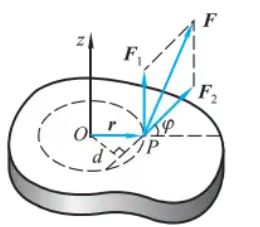
\includegraphics[width=0.3\linewidth]{images/力矩}
	\caption[定轴转动的力矩]{}
	\label{fig:}
\end{figure}
$\mathbf{F_1}$为平行于转轴的力，$\mathbf{F_2}$为垂直于转轴的力，d成为力臂。
$$ |\mathbf{M_z}|=|\mathbf{F_2}\mathbf{r}\sin\varphi|=|\mathbf{F_2}d|$$

\subsection{角速度}

1.角速度为\textbf{矢量}，$\mathbf{v}=\mathbf{\omega}\mathbf{r} $

2.角速度的方向用右手螺旋定则判断，且对于定轴转动，角速度方向始终与转轴平行。

\subsection{转动惯量和定轴转动定律}

下给出简要推导：

取刚体中任一质量元$\Delta m$,其受外力为$\mathbf{F_{ei}}$,受内力为$\mathbf{F_{i}}$

由牛顿第二定律$$\mathbf{F_{ei}}+\mathbf{F_{i}} ={\Delta m}\mathbf{a_i}$$

在自然坐标系中$${F_ei}\sin\varphi_i+F_{i}\sin\theta_i= \Delta m\mathbf{r_i}\mathbf{\alpha}$$

同乘$\mathbf{r_i}$，并对质量元累加$$\sum_{i=1}^{n}{F_{ei}}\sin\varphi_i+\sum_{i=1}^{n}F_{i}\sin\theta_i=\sum_{i=1}^{n}\Delta m_i{r_i}^2\alpha$$

对于刚体而言，内力作用产生的相对位移为0，因此内力矩之和为零。

因此$$\mathbf{M_z}=J\mathbf{\alpha}=J\dfrac{\mathrm{d\omega}}{\mathrm{d}t}$$
\begin{figure}[h]
	\centering
	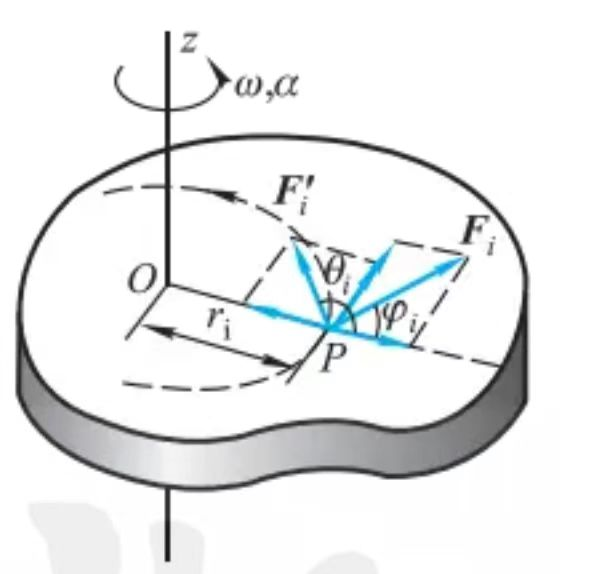
\includegraphics[width=0.3\linewidth]{images/定轴转动定律}
	\caption{定轴转动定律}
	\label{fig:}
\end{figure}

\subsubsection{转动惯量}

1.$J=\sum_{i=1}^{n}\Delta m_i{r_i}^2 $，单位为$kg\cdot m^2$

2.当刚体为质量连续体时，$J=\int r^2\mathrm{d}m $(其中r为质元$\mathrm{d}m $到轴的距离)

3.转动惯量取决于刚体的形状大小、质量分布和转轴的位置。

\subsubsection{转动与平动的联系}

对比牛顿第二定律和定轴转动定律
$\left\{
\begin{aligned}
	\mathbf{F}=m\mathbf{a}\\
	\mathbf{M}=\mathbf{J}\alpha
\end{aligned}
\right.$

其中，m成为惯性质量，是平动惯性的量度，而$\mathbf{J}$也可视作定轴转动刚体的一种特性，是刚体转动惯量的量度；且牛顿第二定律两边同乘$\mathbf{r}$,即为定轴转动定律，因此，可将定轴转动定律视作转动下的牛顿第二定律。

\subsubsection{平行轴定理}

\textbf{刚体对任一转轴的转动惯量$\mathbf{J}$等于通过质心轴的转动惯量$\mathbf{J_c}$加上$\mathbf{mh^2}$,其中$\mathbf{h}$ 为两平行轴之间的距离。}

$$\mathbf{J}=\int(x+h)^2\mathrm{d}m=\int x^2\mathrm{d}m+\int h^2\mathrm{d}m+2h\int x\mathrm{d}m=\mathbf{J_c}+mh^2 $$

(当刚体是绕定轴转动的匀质对称刚体时，$\int x\mathrm{d}m=0 $)

\subsubsection{常见模型的转动惯量}

下给出薄圆盘的转动惯量证明，刚体的转动惯量一般都可由一般模型和平行轴定理推导而得。

圆盘的质量为m,半径为R,设圆盘面密度为$\sigma$，则$\sigma=\dfrac{m}{\pi R^2}$,取宽度为$\mathrm{d}r $的圆环，则有该圆环质量$\mathrm{d}m=(2\pi r)\mathrm{d}r$,则
$$\mathbf{J}=\int r^2\mathrm{d}m=\int_{0}^{R}2\pi\sigma r^3\mathrm{d}r=\dfrac{\pi\sigma R^4}{2}=\frac{1}{2}mR^2$$

\begin{figure}[h]
	\centering
	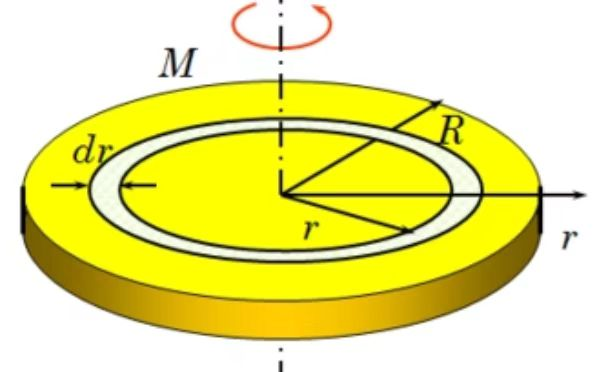
\includegraphics[width=0.2\linewidth]{images/薄圆盘转动惯量}
	\caption[薄圆盘转动惯量]{}
	\label{fig:}
\end{figure}
下为常见刚体转动惯量（书P118-119)
\begin{figure}[h]
	\centering
	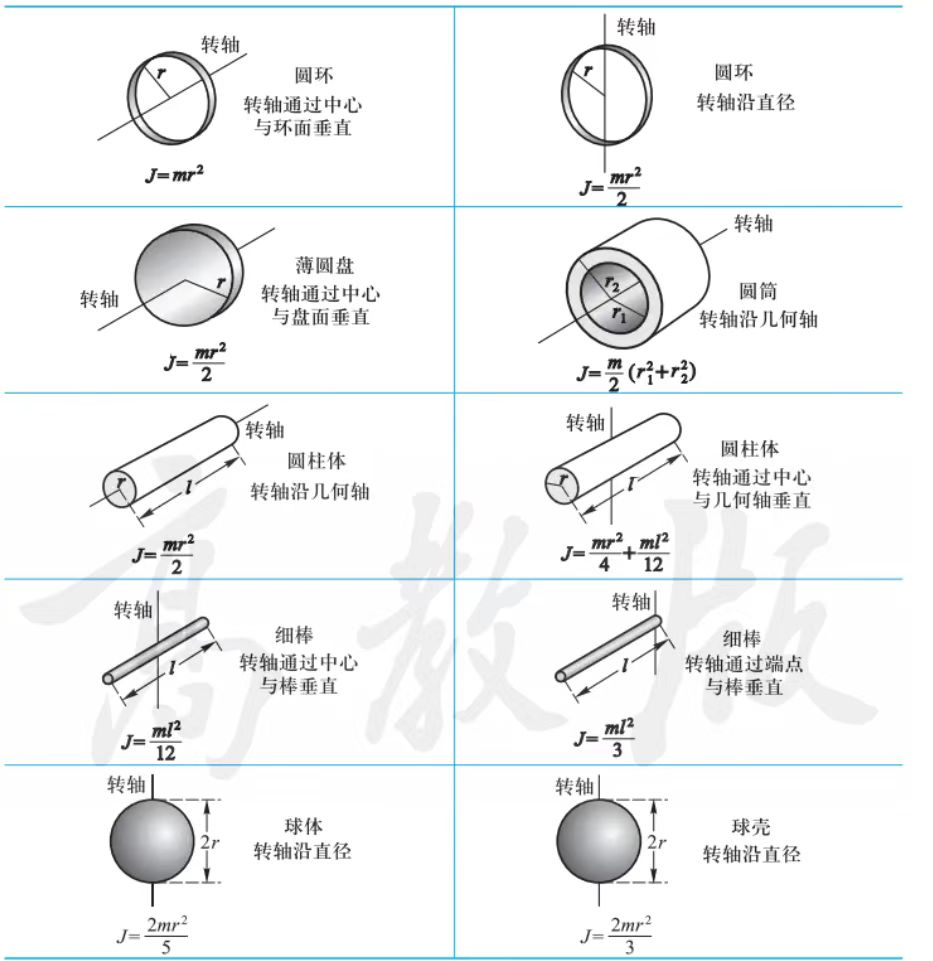
\includegraphics[width=0.9\linewidth]{images/转动惯量模型}
	\caption[转动惯量模型]{}
	\label{fig:}
\end{figure}


\section{定轴转动中的功能关系}

\begin{definition}[力矩的功]
	
刚体定轴运动中，外力做功仅包括垂直转轴平面内分量。

已知力矩 $M_i  = F_irisin\phi \qquad$  角位移为$ \theta \qquad$

则合外力做功为$$A = \sum A_i = \sum \int_{\theta_0}^{\theta} M_i d\theta = \int_{\theta_0}^{\theta}(\sum M_i)d\theta = \int_{\theta_0}^{\theta}Md\theta \qquad $$ 
式中 $M = \sum M_i$ 为刚体所受到的合外力矩。

\end{definition}

\begin{definition}[刚体转动惯量]
$J = \sum m_ir_i^2$
\end{definition}

\begin{definition}[刚体转动动能]
$E_k = \frac{1}{2} J \omega^2$
\end{definition}

\begin{definition}[刚体定轴转动动能定理]
合外力矩对刚体所做的功等于刚体动能增量
\end{definition}
\begin{supplement}
工程上的应用：转动惯量很大的飞轮储存转动动能
\end{supplement}



\section{进动与流体}
\begin{definition}[进动]
    \textbf{进动}是指刚体绕轴旋转时，旋转轴绕另外一个轴旋转的回转现象，如图\ref{pic:3.5-1}所示.
\end{definition}
\begin{figure}[hb]
    \begin{center}
        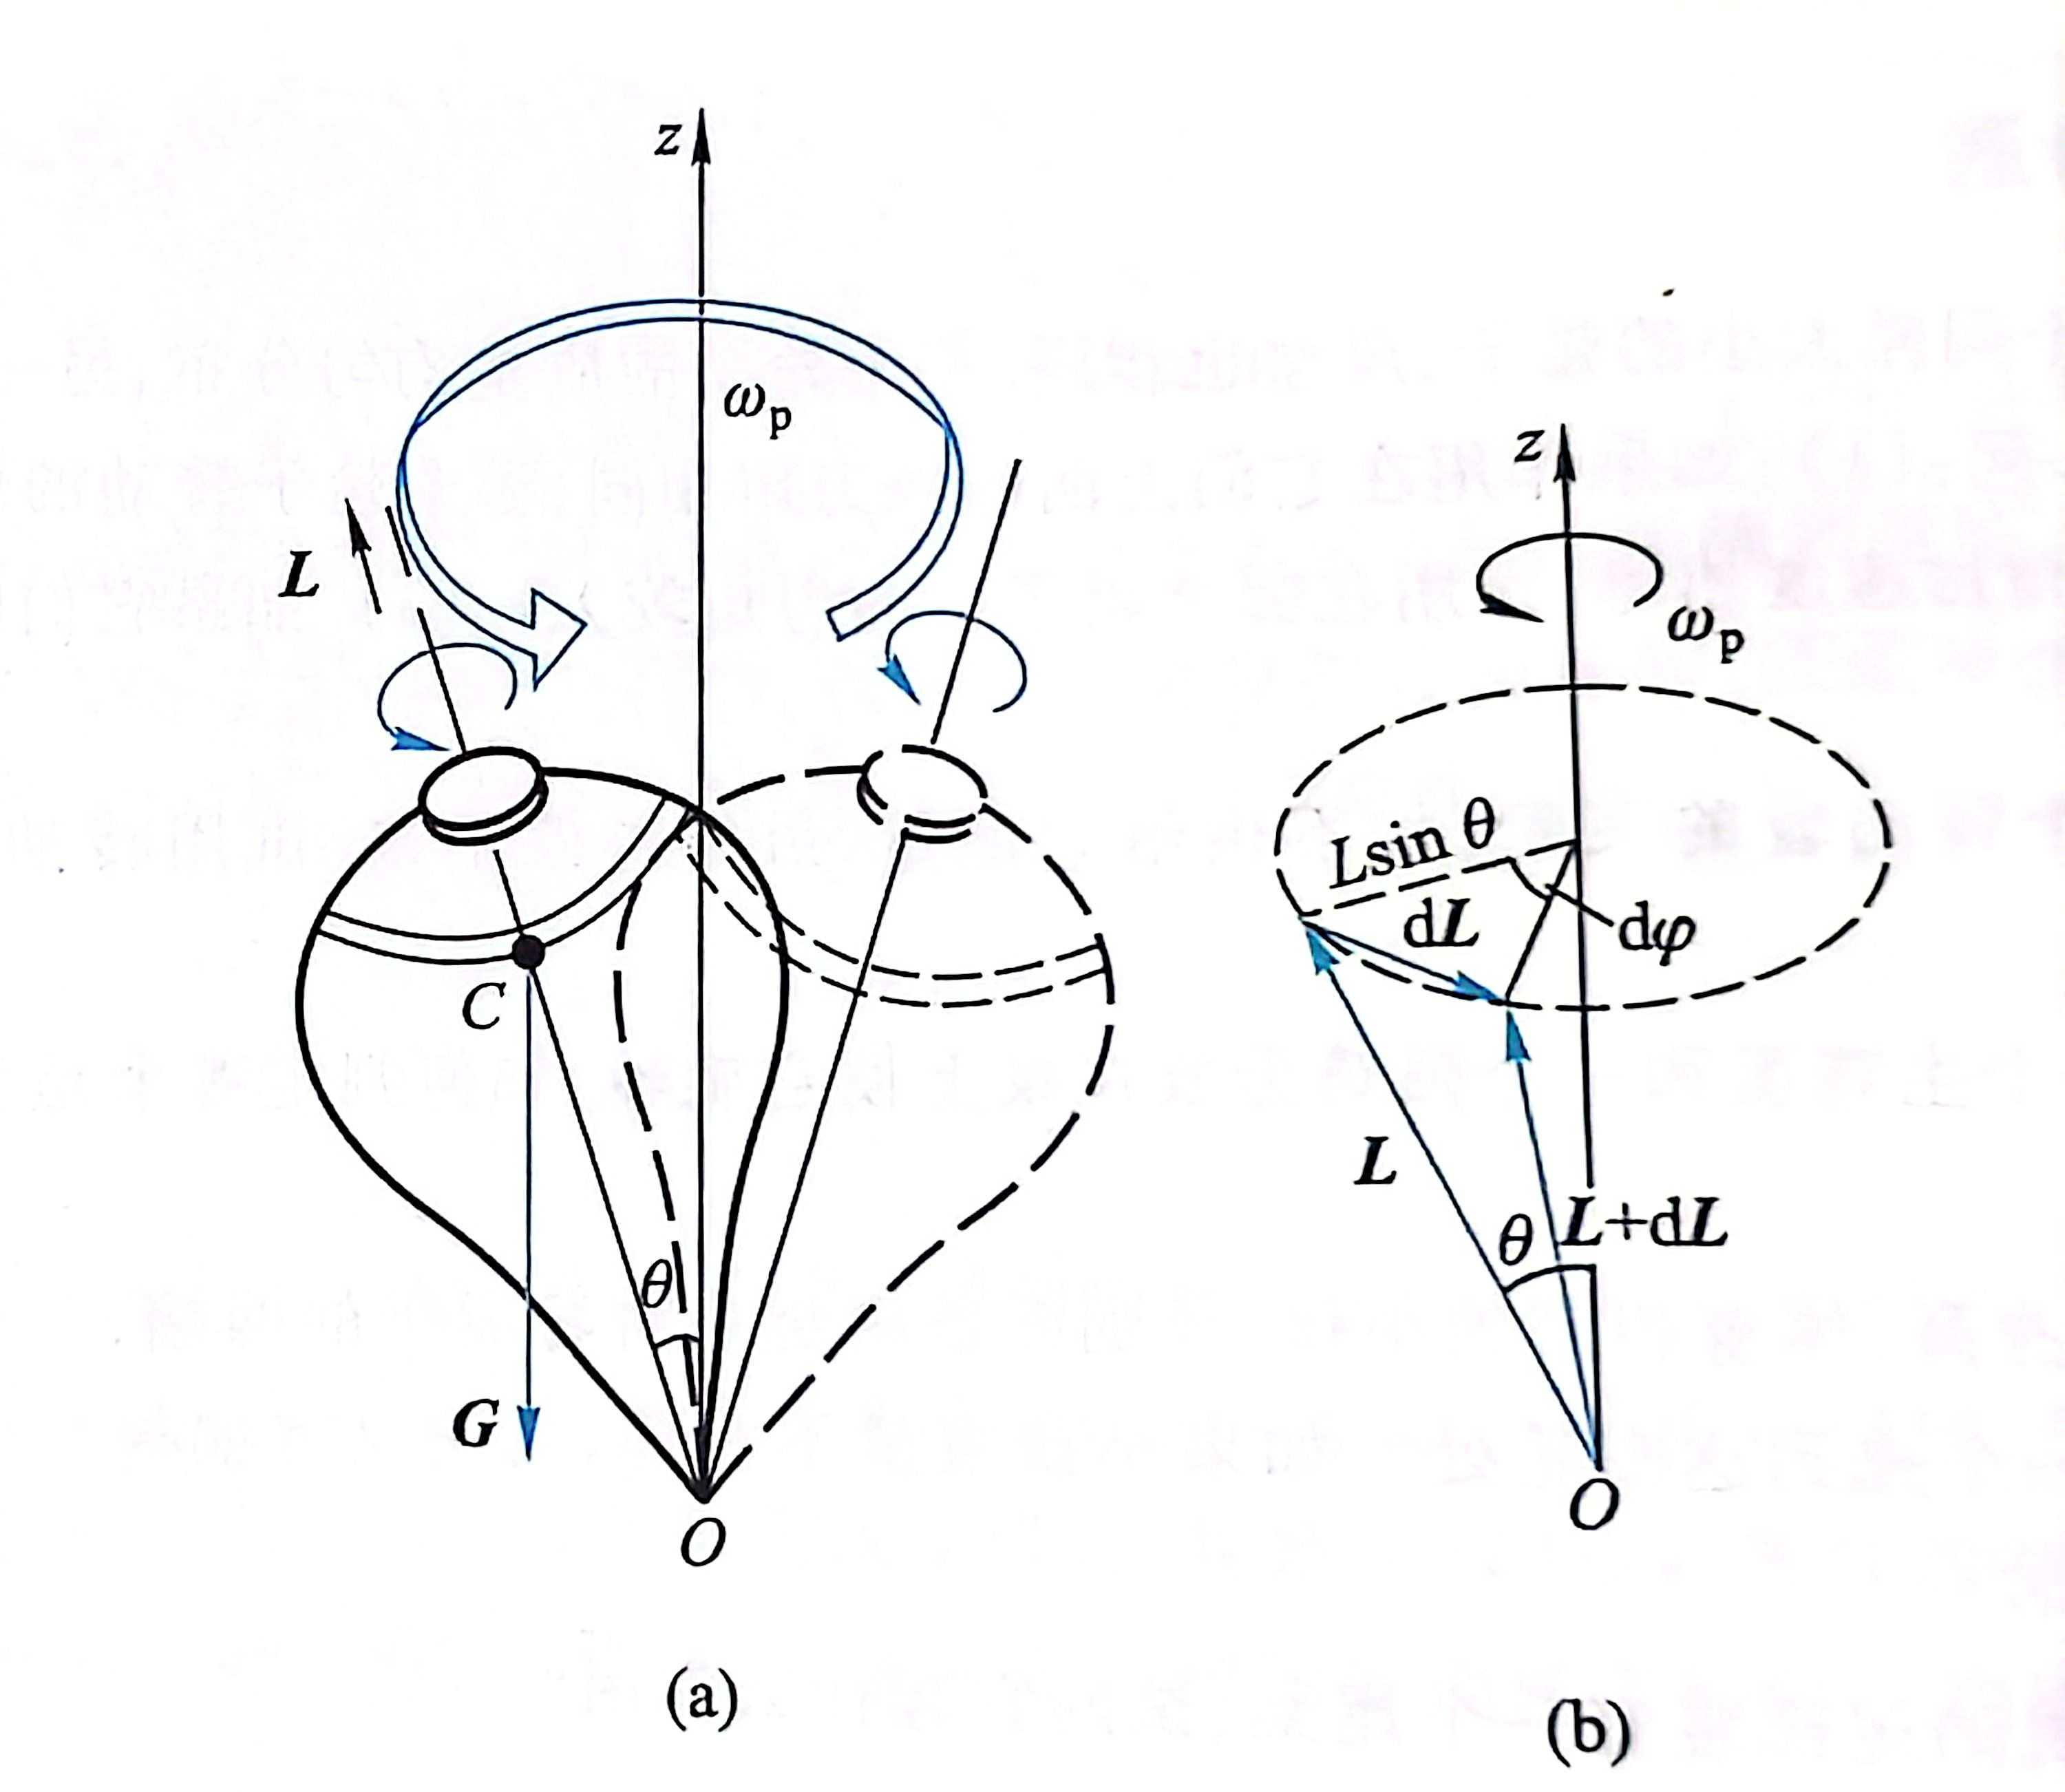
\includegraphics[width=0.6\textwidth]{images/3-5-1.jpg}
        \caption{进动示意图}
        \label{pic:3.5-1}
    \end{center}
\end{figure}

进动是由作用在刚体上与旋转轴垂直的外力矩引起的，一般出现在自转角速度较大的情况下.进动角速度可由公式\ref{equ:3.5-1}确定.

\begin{equation}
    \omega_p=\dfrac{M}{J\omega \sin\theta}
    \label{equ:3.5-1}
\end{equation}

在自转角速度较小的情况下，刚体可能还会\textbf{章动}，在此不详细介绍.

\begin{definition}[定常流动]
    流场中各点流速不随时间变化的流动称为\textbf{定常流动}.
\end{definition}

对于不可压缩，没有黏性的\textbf{理想流体}，有伯努利方程，表明作定常流动的流体中，在同一流管中任何一点处，流体每单位体积的动能和势能以及在该处的压强之和为常量.在工程中，该方程常表示为公式\ref{equ:3.5-2}.
\begin{equation}
    \dfrac{p}{\rho g}+\dfrac{v^2}{2g}+h=Const
    \label{equ:3.5-2}
\end{equation}
其中，公式\ref{equ:3.5-2}左端各项依次称为压力头（表征压力）、速度头（表征动能）、水头（表征势能），公式右端表示一个（具有长度量纲的）常数.
\part{近代物理}
\chapter{狭义相对论}
\section{伽利略相对性原理~伽利略变换}

\subsection{伽利略相对性原理}

\textbf{根据实验现象可以得出，力学规律对于一切惯性系都是等价的。}

\subsection{伽利略变换}

事件：某一时刻发生在空间某一点的一个事例。

设两个惯性系S系和S'系，且S'系相对于S系以速度$\mathbf{u}$沿X轴方向做匀速直线运动。

如果某时刻在空间某一点P发生了一事件，S和系的观测者分别观测这一事件，且规定当S系和S'系中原点重合时，两惯性系开始计时，即$t_{0}=t'_{0}$。

则可以得到正变换
$\left\{
\begin{aligned}
	x'=x-\mathbf{u}t\\
	y'=y\\
	z'=z\\
	t'=t
\end{aligned}
\right.$

和负变换
$\left\{
\begin{aligned}
	x=x'+\mathbf{u}t'\\
	y=y'\\
	z=z'\\
	t=t'
\end{aligned}
\right.$

\subsection{经典力学时空观}

1.时间绝对性:时间间隔与惯性系选择无关。

2.空间绝对性:空间间隔与惯性系选择无关。

3.时间、长度、质量是绝对的，同时性是绝对的，坐标和速度是相对的。
\section{狭义相对论基本原理与洛伦兹变换}
\subsection{狭义相对论基本原理}
成立前提：在彼此相对作匀速直线运动的\textbf{惯性参考系}中。

\begin{enumerate}
	\item \textbf{相对论原理：}物理定律在一切惯性参考系中都具有相同的数学表达形式。（所有惯性参考系对于描述物理现象都是等价的）
	\item \textbf{光速不变原理：}在彼此相对作匀速直线运动的任一惯性参考系中，所测得的光在真空中的传播速度都是相等的。
\end{enumerate}

\subsection{洛伦兹变换}
反映了两个相对作匀速直线运动的惯性参考系中的时空变换关系。

变换关系满足
$$\begin{cases}
	x^{'}=\frac{x-ut}{\sqrt{1-(\frac{u}{c})^2}}\\
	y^{'}=y\\
	z^{'}=z\\
	t^{'}=\frac{t-\frac{ux}{c^2}}{\sqrt{1-(\frac{u}{c})^2}}
\end{cases}$$
或
$$\begin{cases}
	x=\frac{x^{'}+ut}{\sqrt{1-(\frac{u}{c})^2}}\\
	y=y^{'}\\
	z=z^{'}\\
	t=\frac{t^{'}+\frac{ux}{c^2}}{\sqrt{1-(\frac{u}{c})^2}}
\end{cases}$$
\begin{enumerate}
	\item 洛伦兹变换与伽利略变换：当$u\ll c$时，即比值$\beta=\frac{u}{c}$很小时，洛伦兹变换变换就转化为伽利略变换。
	\item 相对论并没有把经典力学推翻，只是揭示了它的局限性。
	\item 相对论指出物体的速度不能超过真空中的光速。
\end{enumerate}


	
	
\section{相对论速度变换}
	
\begin{theorem}[相对论速度变换公式]


令$\beta= \frac{u}{c}$

依据：洛伦兹坐标变化

当物体沿X方向运动时，K系中速度表达式为
$$v_x = \frac{dx}{dt}	$$
K'系中速度表达式为
$$v'_x = \frac{dx'}{dt'} =  \frac{dx'-udt}{dt'-\frac{u}{c^2}dx} =\frac{v_x-u}{1-\frac{u}{c^2} v_x}	$$

$$v'_y =\frac{V_y(1-\beta^2)^\frac{1}{2}}{1-\frac{u}{c^2}v_x}	$$


逆变换

$$ v_x = \frac{v'_x + u} {1 + \frac{u} {c^2}v'_x } $$

$$v_y =\frac{v_y'(1-\beta^2)^\frac{1}{2}}{1+\frac{u}{c^2}v_x'}	$$

$v_z$和$v_y$同理
\end{theorem}

\begin{note}
	适用范围：$u$(惯性系间相对速度)和$v$接近光速时。
	
	相对论速度变换遵循光速不变原理。
\end{note}



\part{电磁学}
\chapter{静电场}
\section{电荷~库仑定律}

\subsection{电荷}

1.\textbf{电荷量}：表示物体所带电荷多寡的物理量。

2.物体所带电荷只有正电荷和负电荷,同号电荷相互排斥，异号电荷相互吸引。

\subsection{电荷守恒定律}

1.\textbf{起电}：通过某种作用，使该物体内电子不足或过多而呈带电状态。

2.\textbf{电荷守恒定律}：在一个与外界没有电荷交换的系统内，无论经过怎样的物理过程，系统内正、负电荷的代数和总保持不变。

3.电荷是相对论不变量，即电荷量与运动无关。

\subsection{电荷的量子化}

电荷量这种只能取分立的、不连续量值的性质，称为电荷量子化。

一般近似取$e=1.602176634×10^{-19}$

\subsection{库仑定律}

1.库仑扭秤实验总结出了\textbf{库仑定律}：两个静止点电荷之间相互作用力的大小与这两个点电荷的电荷$q_{1}$和$q_{2}$的乘积成正比，而与这两个点电荷之间的距离$r_{12}$的二次方成反比，作用力的方向，沿着这两个点电荷的连线。

$$\mathbf{F}=k\frac{q_{1}q_{2}}{{r_{12}}^{2}}$$
$$k=\frac{1}{4\pi\varepsilon_{0}}$$
则$$\mathbf{F_{12}}=\mathbf{F_{21}}=\frac{1}{4\pi\varepsilon_{0}}\frac{q_{1}q_{2}}{{r_{12}}^{2}}\mathbf{e_{r_{12}}} $$

2.适用条件：真空、静止、点电荷

\subsection{静电力的叠加原理}

1.\textbf{静电力叠加原理}：当空间有两个以上的点电荷时，作用在某一点电荷上的总静电力等于其他各点电荷单独存在时，对该点电荷所施静电力的矢量和。

$$\mathbf{F}=\sum_{i=1}^{n}\mathbf{F_{i}}=\frac{1}{4\pi\varepsilon_{0}}\sum_{i=1}^{n}\frac{qq_{i}}{{r_{i}}^{2}}\mathbf{e_{r_{i}}}$$

2.库伦定律只适用于点电荷,将带电体看作是由许多电荷元组成的，根据库仑定律和叠加原理，则可求解带电体之间的相互作用力。

\section{静电场\quad 电场强度}
\subsection{电场}
电场：电荷周围存在的一种特殊物质。分布在一定范围的空间里，具有能量、动量等属性，并通过交换场量子来实现相互作用的传递。电磁场的媒介子是光子。

电场力：电场对处在其中的其他电荷的作用力。两个电荷之间的相互作用力本质上是一个电荷的电场作用在另一个电荷上的电场力。

静电场：相对于观察者为静止的点电荷在其周围所激发的电场。

\subsection{电场强度}
\subsubsection{检验电荷}
\begin{enumerate}
	\item 所带电荷量充分小。
	\item 线度小到可以被看作点电荷。
\end{enumerate}
用检验电荷所受的力与检验电荷所带电荷量之比，可以定义电场强度。

\subsubsection{电场强度}
定义：电场中某点的电场强度的大小等于单位电荷在该点所受的力的大小，其方向为正电荷在该点的受力方向。
$$\vec{E}=\frac{\vec{F}}{q_0}$$

符号：$\vec{E}$

单位：$N/C$，$V/m$

标矢性：矢量

\subsection{电场强度的叠加原理}
点电荷系在空间任一点所激发电场的总电场强度等于各个点电荷单独存在时在该点各自所激发电场的电场强度的矢量和。（简称场强叠加原理）

利用这一原理可以计算任意带电体所激发电场的电场强度，因为任何带电体都可以看作许多点电荷的集合。

\subsection{电场强度的计算}
\subsubsection{点电荷}
对于一个静止的点电荷$q$（场源电荷），距$q$为$r$的$P$点（场点）的电场强度为
$$\vec{E}=\frac{1}{4\pi\varepsilon_0}\frac{q}{r^2}\vec{e_r}$$

式中$\vec{e_r}$是由点电荷$q$指向$P$点的单位矢量。

\subsubsection{点电荷系}
$$\vec{E}=\vec{E_1}+\vec{E_2}+\dots+\vec{E_n}=\sum_{i=1}^n{\frac{q_i}{4\pi\varepsilon_0 r_i^2}\vec{e_ri}}$$

\subsubsection{连续分布电荷}
把带电体看成许多极小的连续分布的电荷元$\mathbf{d}q$的集合，每一个电荷元$\mathbf{d}q$都当作点电荷来处理。
$$\mathbf{d}\vec{E}=\frac{1}{4\pi\varepsilon_0}\frac{\mathbf{d}q}{r^2}\vec{e_r}$$
$$\vec{E}=\int\mathbf{d}\vec{E}=\frac{1}{4\pi\varepsilon_0}\int\frac{\mathbf{d}q}{r^2}\vec{e_r}$$

\subsubsection{经典模型}
\begin{itemize}
	\item 电偶极子
	
	电偶极子：两个大小相等符号相反的点电荷$+q$和$-q$，当它们之间的距离$l$比所考虑的场点到它们的距离小得多时，这一电荷系统称为电偶极子。
	
	轴线：取从负电荷指向正电荷的矢量$\vec{l}$的方向作为轴线的正方向。
	
	电偶极矩（电矩）：$\vec{p}=q\vec{l}$
	
	对轴线的延长线上的某点A：$\vec{E_A}=\frac{1}{4\pi\varepsilon_0}\frac{2\vec{p}}{y^3}$
	
	对中垂线上的某点A：$\vec{E_A}=-\frac{1}{4\pi\varepsilon_0}\frac{\vec{p}}{x^3}$
	
	\item  均匀带电直棒
	
	长度为$L$，总电荷量为$q$，电荷线密度$\lambda=q/L$。棒外一点$P$离开直棒的垂直距离为$a$，$P$点和直棒两端的连线与直棒之间的夹角分别是$\theta_1$和$\theta_2$。
	
	$P$点的电场强度：$E=\frac{\lambda}{4\pi\varepsilon_0}\sqrt{2-2\cos(\theta_1-\theta_2)}$，与$Ox$轴的夹角$\alpha=\arctan\frac{\cos\theta_1-\cos\theta_2}{\sin\theta_2-\sin\theta_1}$
	
	无限长均匀带电直棒（或$a\ll L$时）：$E=\frac{\lambda}{4\pi\varepsilon_0}$（$\theta_1=0$，$\theta_2=\pi$）
	
	\item 带电圆环
	
	半径为$R$，总电荷量为$q$。
	
	轴线上一点$P$处的电场强度：$E=\frac{qx}{4\pi\varepsilon_0(x^2+R^2)^{3/2}}$。若$q$为正电荷，沿$Ox$轴正方向：若$q$为负电荷，沿$Ox$轴负方向。
	
	当$x\gg R$时：$E=\frac{q}{4\pi\varepsilon_0 x^2}$
	
	\item 带电圆盘
	
	半径为$R$，面密度为$\sigma$。
	
	轴线上一点$P$处的电场强度：$E=\frac{\sigma}{2\varepsilon_0}(1-\frac{x}{\sqrt{R^2+x^2}})$。若$\sigma>0$，沿$Ox$轴正方向；若$\sigma<0$，沿$Ox$轴负方向。
	
	当$R\gg x$时：：$E=\frac{\sigma}{2\varepsilon_0}$
	
	当$x\gg R$时：$E=\frac{q}{4\pi\varepsilon_0 x^2}$
\end{itemize}

\subsection{电场对电荷的作用力}
$$\vec{F}=q\vec{E}$$
$q>0$时，$\vec{F}$与$\vec{E}$同向；$q<0$时，$\vec{F}$与$\vec{E}$反向。

\subsection{电场线\quad 电场强度通量}
\subsubsection{电场线}
 电场线上每一点的切线方向都与该点处的电场强度$\vec{E}$的方向一致。任一点电场线的密度与该点的电场强度的大小成正比。
 
 \begin{enumerate}
 	\item 电场线起始于正电荷（或来自无穷远处），终止于负电荷（或伸向无穷远处），不会在没有电荷的地方中断（电场强度为零的奇异点除外）。
 	\item 电场线不能形成闭合曲线。
 	\item 任何两条电场线不会相交。
 \end{enumerate}
 
 \subsubsection{电场强度通量}
 定义：在均匀电场中取一个想象中的平面。引入面积矢量$\vec{S}$，其大小等于平面的面积$S$，其方向为平面正法线的方向。设平面正法线的单位矢量$\vec{e_n}$与$\vec{E}$成$\theta$角。
 
 如果取电场线的密度等于场强的大小，则通过这一平面的电场线总数等于
 $$\varPhi_e=E\cos\theta S=\vec{E}\cdot\vec{S}$$
 也称作通过该面积的电场强度通量，即$\vec{E}$通量。
 
 \begin{itemize}
 	\item 不均匀电场：
 	
 	把曲面划分为无限多个面积元$\mathbf{d}S$，在每一个无限小的面积元$\mathbf{d}S$上电场强度可以认为是均匀的。
 	$$\varPhi_e=\int_{S}\mathbf{d}\varPhi_e=\int_{S}\vec{E}\cdot\mathbf{d}\vec{S}$$
 	
 	\item 闭合曲面：
 	
 	对非闭合曲面，面法线的方向可以取曲面的任一侧。对闭合曲面来说，通常规定自内向外的方向为面积元法线的正方向。
 	
 	所以，在电场线从曲面之内向外穿出时$\vec{E}$通量为正：反之，在电场线从外部穿入曲面时，$\vec{E}$通量为负。
 \end{itemize}

	
	
	\section{静电场的高斯定理}
	
	\begin{definition}[高斯定理]
		在静电场中，通过任意闭合曲面的电场强度通量等于该曲面内电荷量的代数和除以$\varepsilon _{0}$
		
		$$\oint _{S}E\cdot dS=\frac{1}{\varepsilon _{0}}\sum _{i}q_{i}$$
		
	\end{definition}
	
	\begin{note}
		
		闭合球面上的$E$通量与球面所围成的电荷量成正比，与半径无关。
		
		高斯定理说明了电场强度对闭合面通量和场源电荷关系。
		
		闭合曲面外电荷对闭合曲线上各个点电场强度有作用，但对闭合曲面整体$E$通量贡献为$0$。
		
		适用范围：静电场、运动电荷、迅速变化的电场。
	\end{note}
	
应用方法：

一、电荷分布具有某些特殊的对称性，使相应的电场分布具有一定对称性：
\begin{example}
	1:球对称性：点电荷、均匀带点球体。2：轴对称性：均匀带电直线、柱。3：平面对称性：无限大均匀带点平板。
\end{example}

二、高斯面选择要求：

	电场强度垂直于闭合面且大小处处相等/一部分电场强度垂直于闭合面且处处相等，另一部分电场强度与闭合面平行。

\begin{example}
	球对称电场：球半径为R
	
1、$q$均匀分布在整个球体
	
（1）$P$点在球内
	
$$E = \frac{q}{4\pi\varepsilon _{0}r^2}e_r$$

（2）$P$点在球外

$$E = \frac{qr}{4\pi\varepsilon _{0}R^3}e_r$$
2、$q$均匀分布在球面上
（1）$P$点在球内

$$E =0$$

（2）$P$点在球外

$$E = \frac{qr}{4\pi\varepsilon _{0}R^3}e_r$$


\end{example}

\begin{example}
	柱对称电场：
	
（1）$P$点在圆柱内

$$ E=\frac{\lambda}{2\pi \varepsilon _{0}r}e_{r}$$

（2）$P$点在圆柱外

$$E =\frac{\lambda r}{2\pi \varepsilon _{0}R^2}e_{r}$$
\end{example}

\begin{example}
	平面对称电场：
	
$$E = \frac{\sigma}{2\varepsilon_0} e_n$$

一对电荷面密度相等异号的均匀带电无限大电场（电容板）电场强度大小为

$$E = \frac{\sigma}{\varepsilon_0} $$
\end{example}


\section{电场强度与电势的关系}
电场强度与电势的积分关系即为电势与电势差（电压）的定义式（取无穷远处为零势点时可以表示为公式\ref{equ:7.5.1}与公式\ref{equ:7.5.2}）.
\begin{equation}
    V_a=\dfrac{W_a}{q_0}=\int_{a}^{\infty}\bm{E}\cdot \mathrm{d}\bm{l}
    \label{equ:7.5.1}
\end{equation}
\begin{equation}
    U_{ab}0=V_a-V_b=\dfrac{W_a}{q_0}-\dfrac{W_b}{q_0}=\int_{a}^{b}\bm{E}\cdot \mathrm{d}\bm{l}
    \label{equ:7.5.2}
\end{equation}

电场强度与电势的微分关系可以由电场力做功推导，结论是静电场中某点的电场强度在量值上等于该点电势梯度的大小，方向与电势梯度矢量方向相反.换言之，\textbf{电场强度的方向为该点电势降低最快的方向}.公式\ref{equ:7.5.3}给出了这个结论的数学表达.
\begin{equation}
    \bm{E}=-\nabla V=-\dfrac{\mathrm{d}V}{\mathrm{d}\bm{n}}\bm{e}_n=-\mathrm{grad}V
    \label{equ:7.5.3}
\end{equation}

公式\ref{equ:7.5.3}的分量式的意义是：在静电场中，电场强度在任一方向的分量等于该方向电势变化率的负值.
\section{静电场中的导体}
\subsection{静电平衡}
将不带电的金属导体置于电场中，由静电感应现象在表面产生感应电荷，感应电荷不断积累，产生附加电场，最终达到导体内部电场强度处处为零，导体中没有任何电荷作定向运动，此状态称为\textbf{静电平衡}状态.需要注意的是该状态是没有电荷作定向运动而非没有电荷作运动，因为存在分子热运动.建立静电平衡的过程如图\ref{pic:7-6-1}所示.
\begin{figure}[hb]
    \begin{center}
        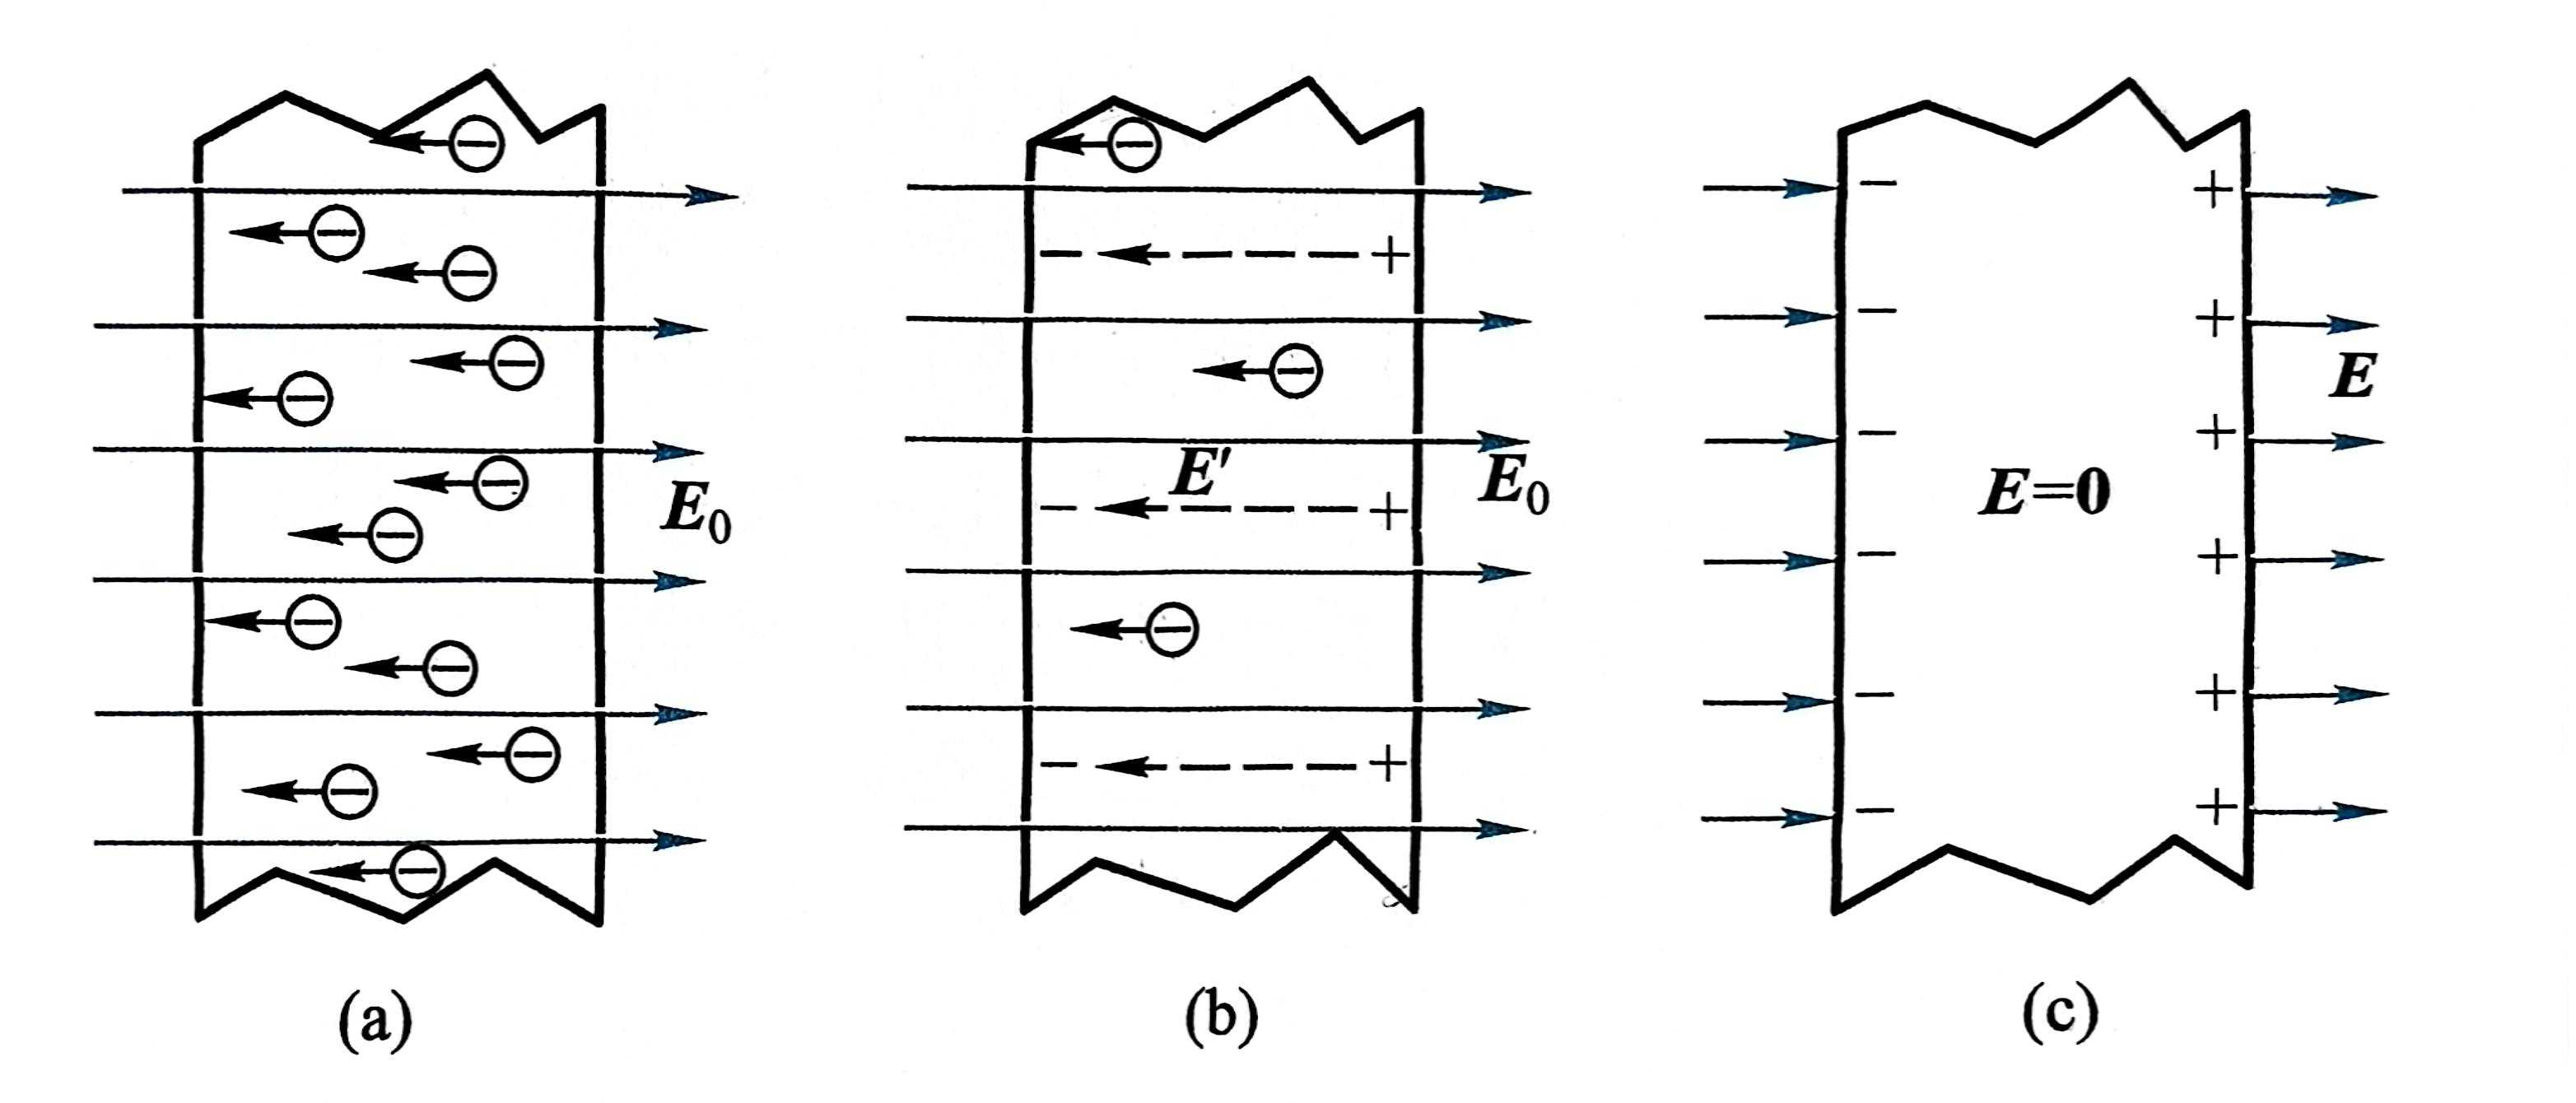
\includegraphics[width=0.6\textwidth]{images/7-6-1.jpg}
        \caption{静电感应过程}
        \label{pic:7-6-1}
    \end{center}
\end{figure}

根据导体静电平衡的条件，如图\ref{pic:7-6-2}所示，我们有以下推论：
\begin{enumerate}
    \item 导体是等势体，其表面是等势面.
    \item 导体表面的电场强度垂直于导体表面.
\end{enumerate}

\begin{figure}[hb]
    \begin{center}
        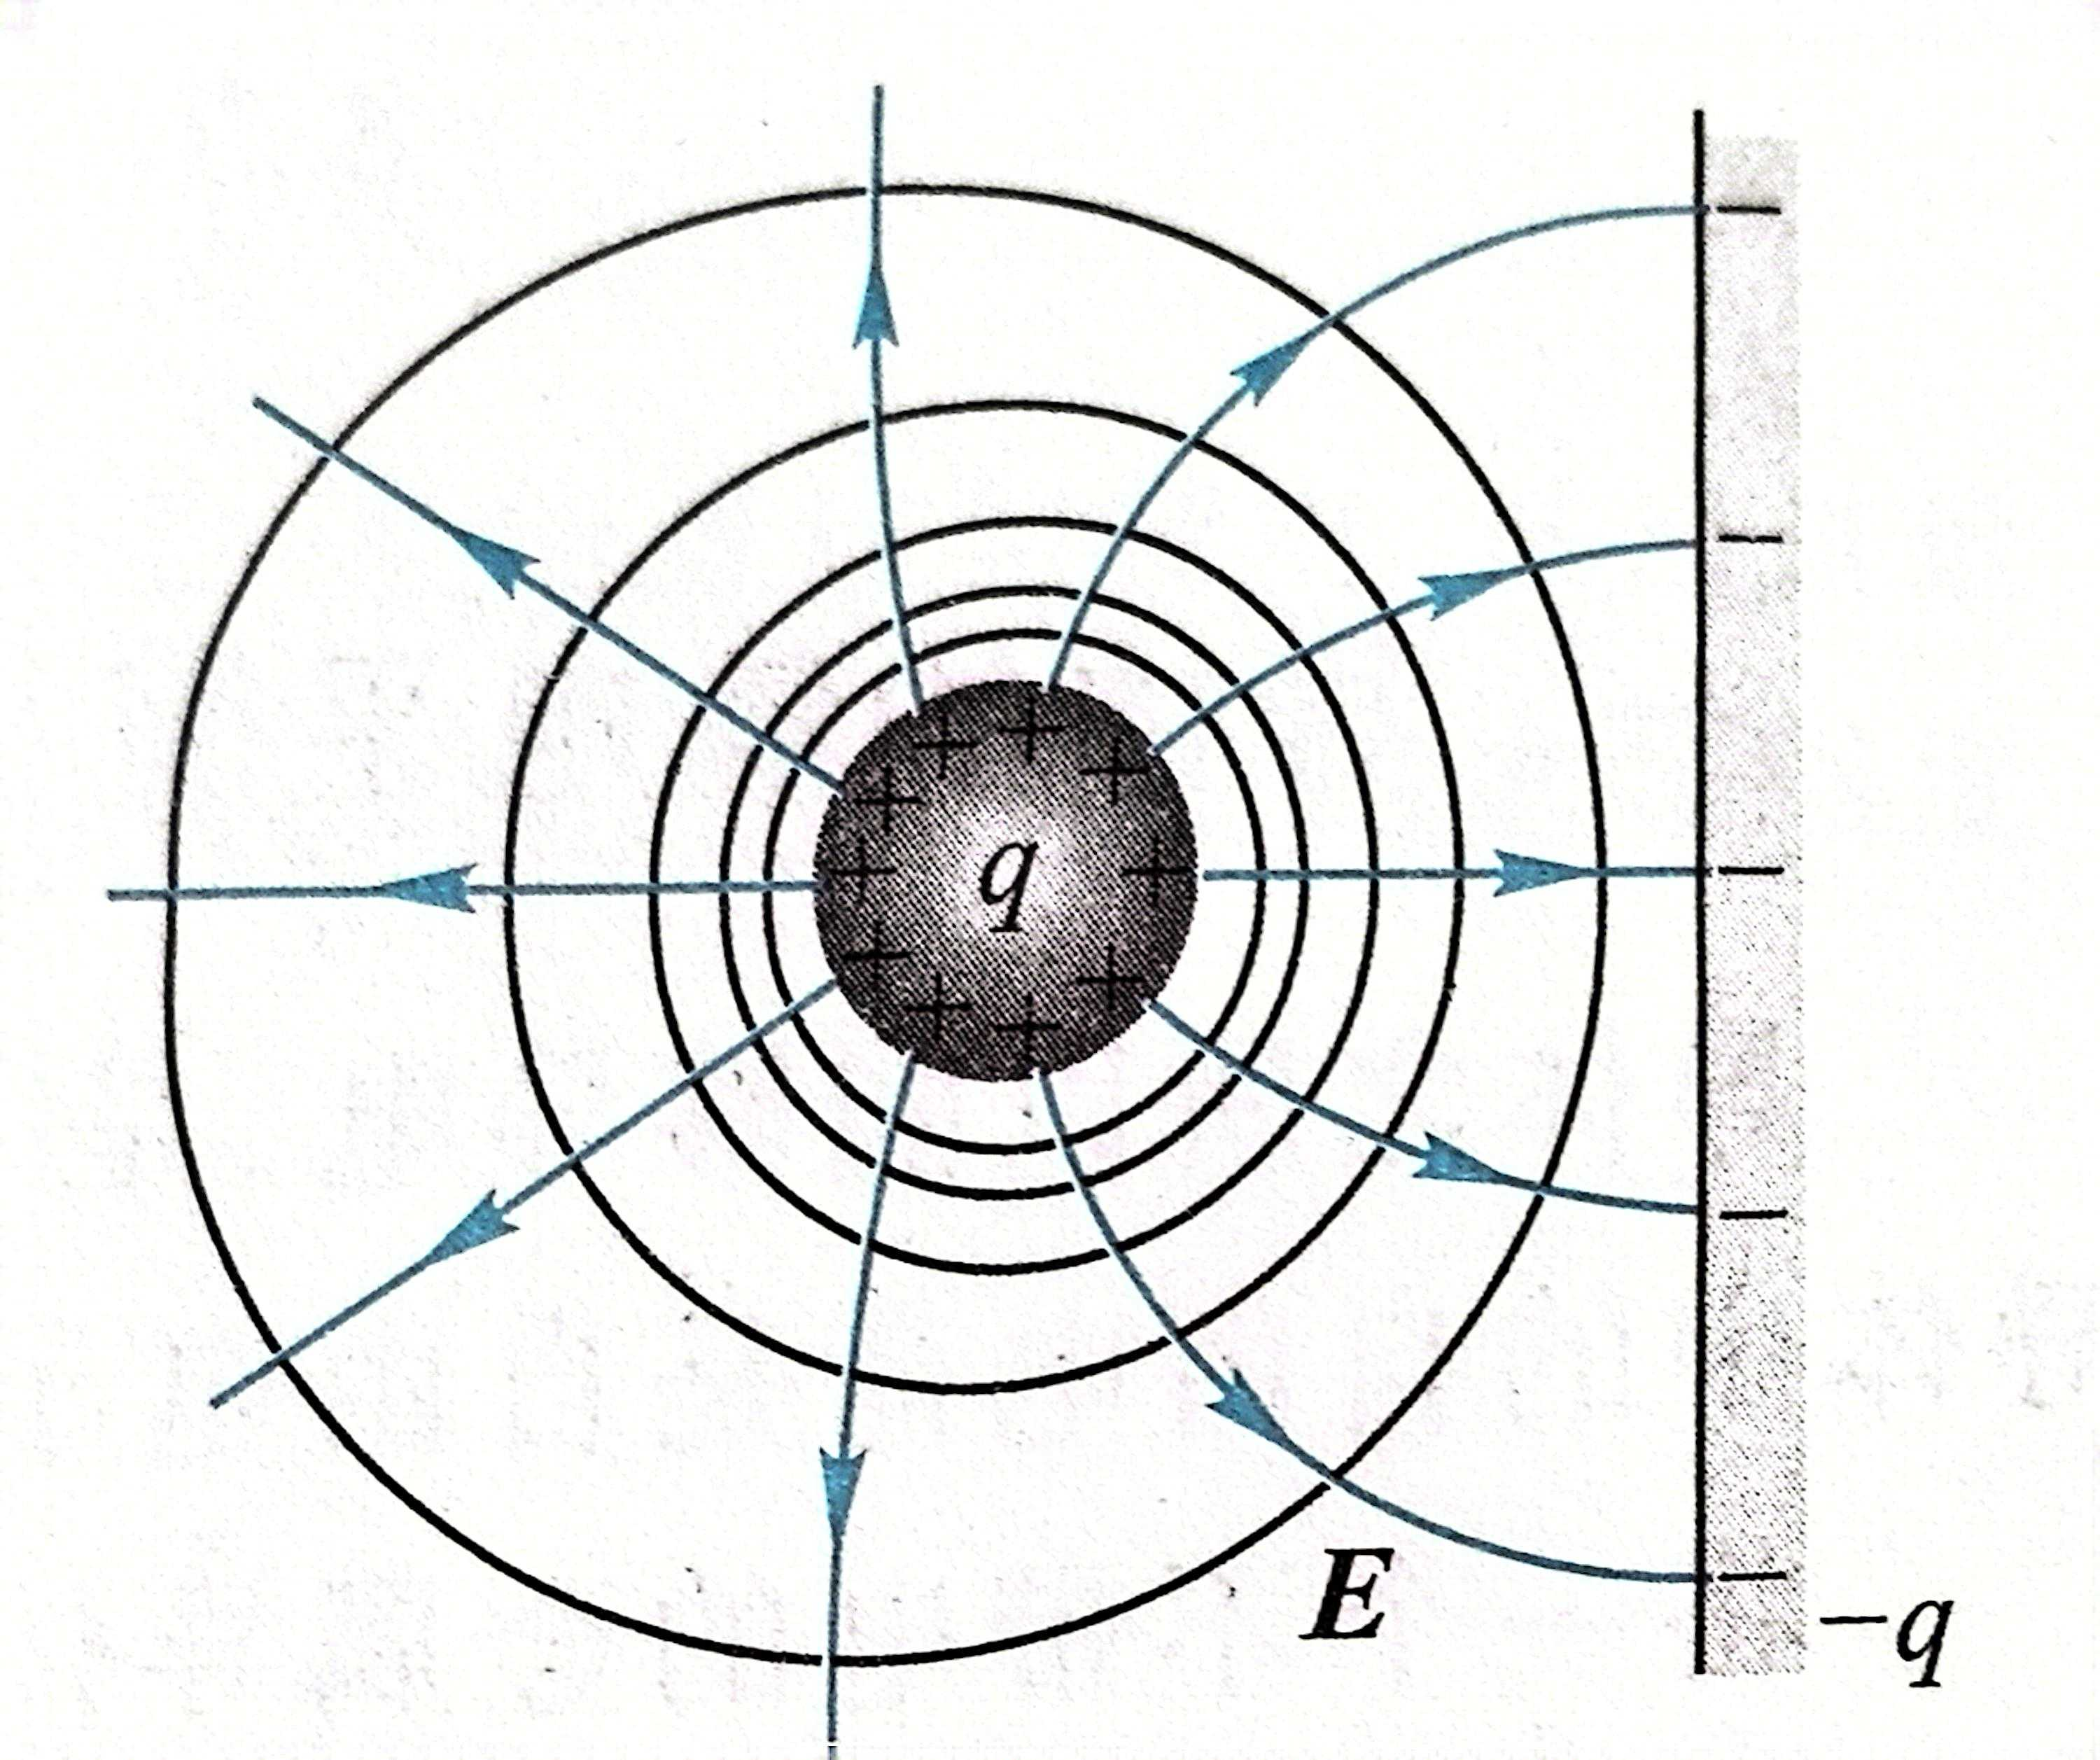
\includegraphics[width=0.4\textwidth]{images/7-6-2.jpg}
        \caption{导体附近电场/等势面分布}
        \label{pic:7-6-2}
    \end{center}
\end{figure}

\subsection{静电平衡时导体上的电荷分布}
根据高斯定理，当带点导体处于静电平衡状态时，电荷只能分布于导体的表面上（仅有感应电荷）.如果导体有空腔，空腔内有电荷时，导体内表面带有与电荷电量相等电性相反的感应电荷；空腔内没有电荷时，导体只有外表面带有感应电荷.


如图\ref{pic:7-6-3}方式取高斯面，由高斯定理，有带电导体表面附近的电场强度公式
\[
\bm{E}=\dfrac{\sigma}{\epsilon_0}\bm{e}_n
\]
\begin{figure}[h]
    \begin{center}
        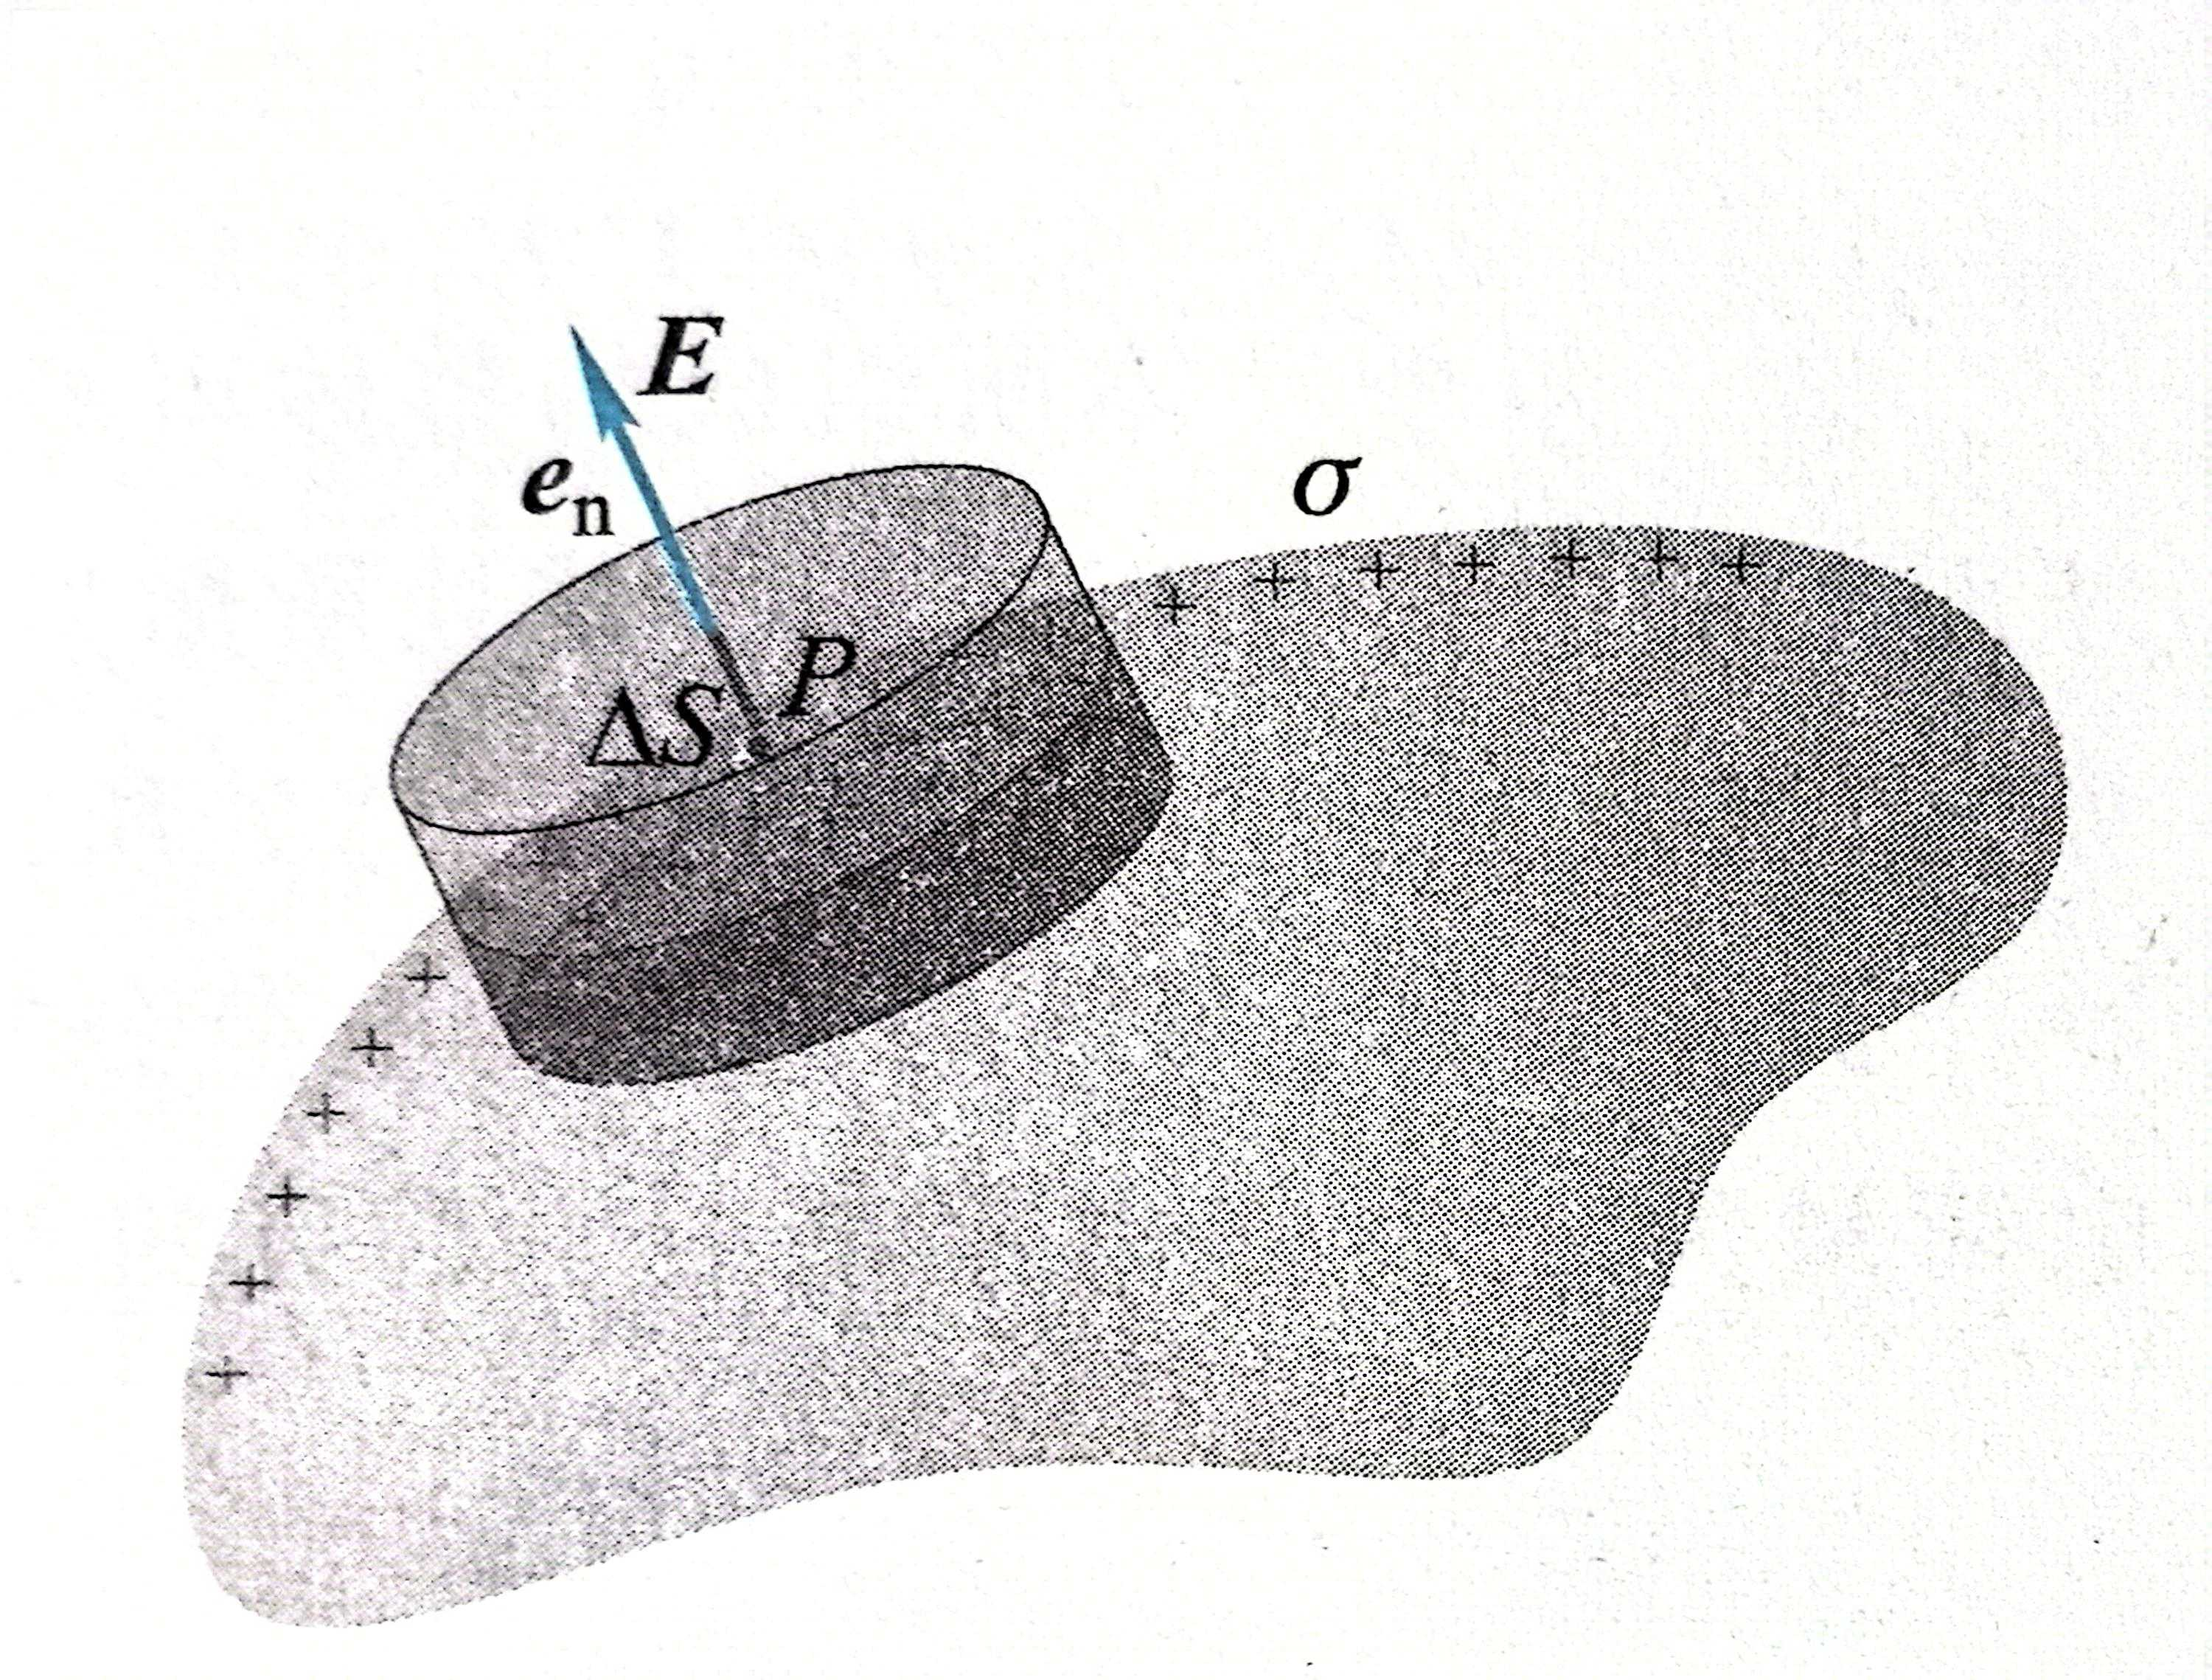
\includegraphics[width=0.4\textwidth]{images/7-6-3.jpg}
        \caption{导体表面附近的高斯面取法}
        \label{pic:7-6-3}
    \end{center}
\end{figure}
\begin{attention}{ }{7.6.1} % 添加标签参数
不要将该公式与无限大均匀带电平面产生的电场强度混淆！事实上，这两个公式说明的是一个问题，只不过电荷面密度代表的含义有所差别.
\end{attention}

对于孤立的带电导体，感应电荷在其表面的分布由其表面曲率确定.曲率越大，电荷分布越密集，此处曲率的符号表征“大小”.只有孤立导体球表面电荷分布均匀.

\subsection{静电屏蔽}
在静电平衡的条件下，导体空腔外的带电体不会影响腔内的电场分布；接地的空腔导体腔内电荷不会影响腔外的电场分布.这就是\textbf{静电屏蔽}效应.
\section{电容器的电容}

\subsection{孤立导体的电容}

1.\textbf{孤立导体的电容}:从理论及实验可知,一个孤立导体的电势V与他所带的电荷量q呈线性关系。
$$C=\frac{q}{V}$$

2.他只与导体的大小、形状和周围介质有关。

3.电容是表征导体储电能力的物理量，其物理意义是使导体升高单位电势所需的电荷量，单位：法拉F。

4.孤立导体球半径为R，带电荷为q，则它的电容为$C=\frac{q}{V}=4\pi\varepsilon_{0}R$。

\subsection{电容器的电容}

根据静电屏蔽的原理，用一个封闭的导体壳B将导体A包围起来，使得导体A及导体壳B构成的一对导体系的电势差$V_{A}-V_{B}$不再受到壳外导体的影响，从而维持恒定，这样一个导体系可以称为电容器。

\begin{figure}[h]
	\centering
	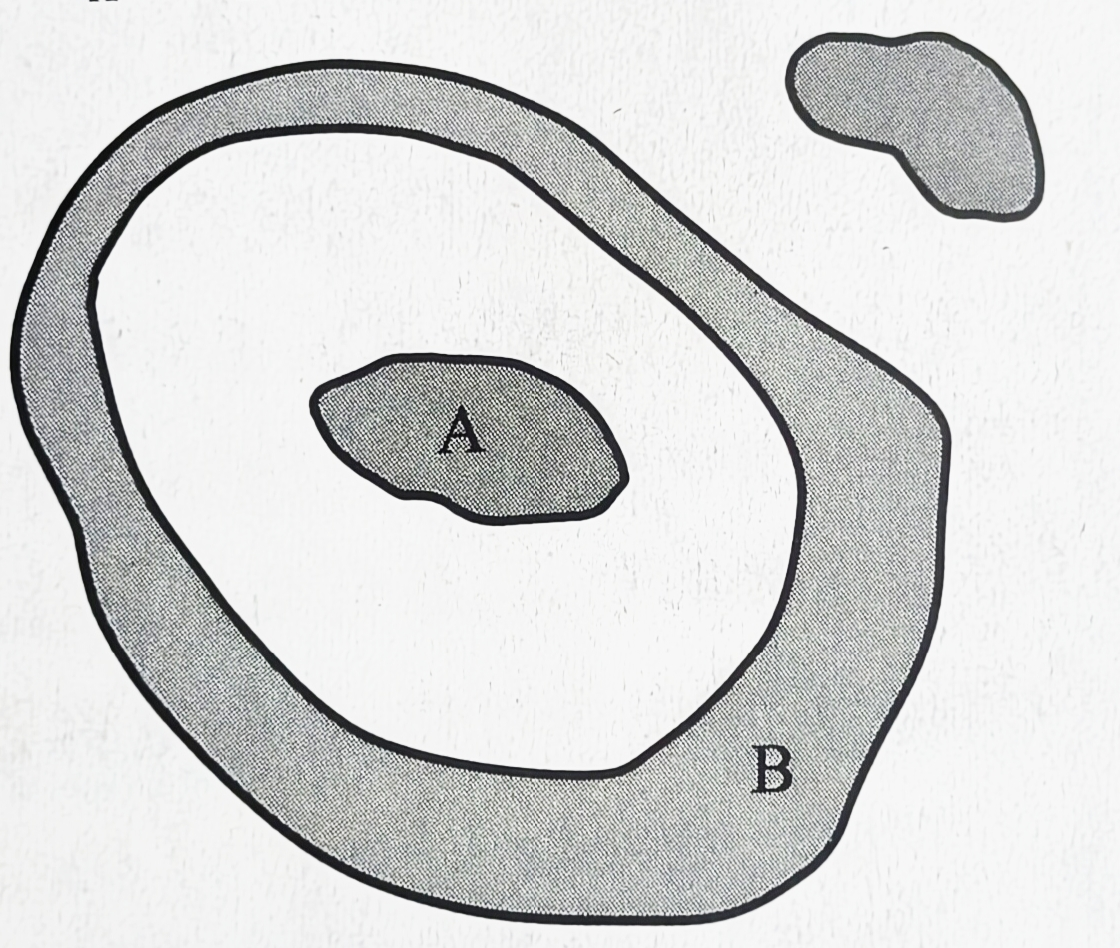
\includegraphics[width=0.3\linewidth]{images/电容器}
	\caption{电容器}
	\label{fig:}
\end{figure}

1.\textbf{电容器的电容}:两导体极板表面上均带有的等量异号电荷q与两极板电势差$\Delta V$的比值。
$$C=\frac{q}{V_{A}-V_{B}}$$

2.实验证明：充有电介质的电容器电容为两板间为真空时的电容$C_{0}$的$\varepsilon_{r}$倍。

其中$\varepsilon_{r}$称为介质的相对电容率或相对介电常量，量纲为1。

\subsection{常见电容器的电容}

\subsubsection{平行板电容器}

两板所带电荷量为q，板间距为d，面积为S，中间充有相对介电常量$\varepsilon_{r} $的电介质，极板的电荷面密度为$\sigma_{0}$。

$$Q=\sigma_{0}S$$

由高斯定理$$D=\sigma_{0}$$

则有$$E=\frac{\sigma_{0}}{\varepsilon_{0}\varepsilon_{r}}$$
$$U=Ed=\int E\mathrm{d}\mathbf{l}$$
$$C=\frac{q}{U}=\frac{\varepsilon_{0}\varepsilon_{r}S}{d}=\varepsilon_{0}\varepsilon_{r}C_{0}$$
\begin{figure}[h]
	\centering
	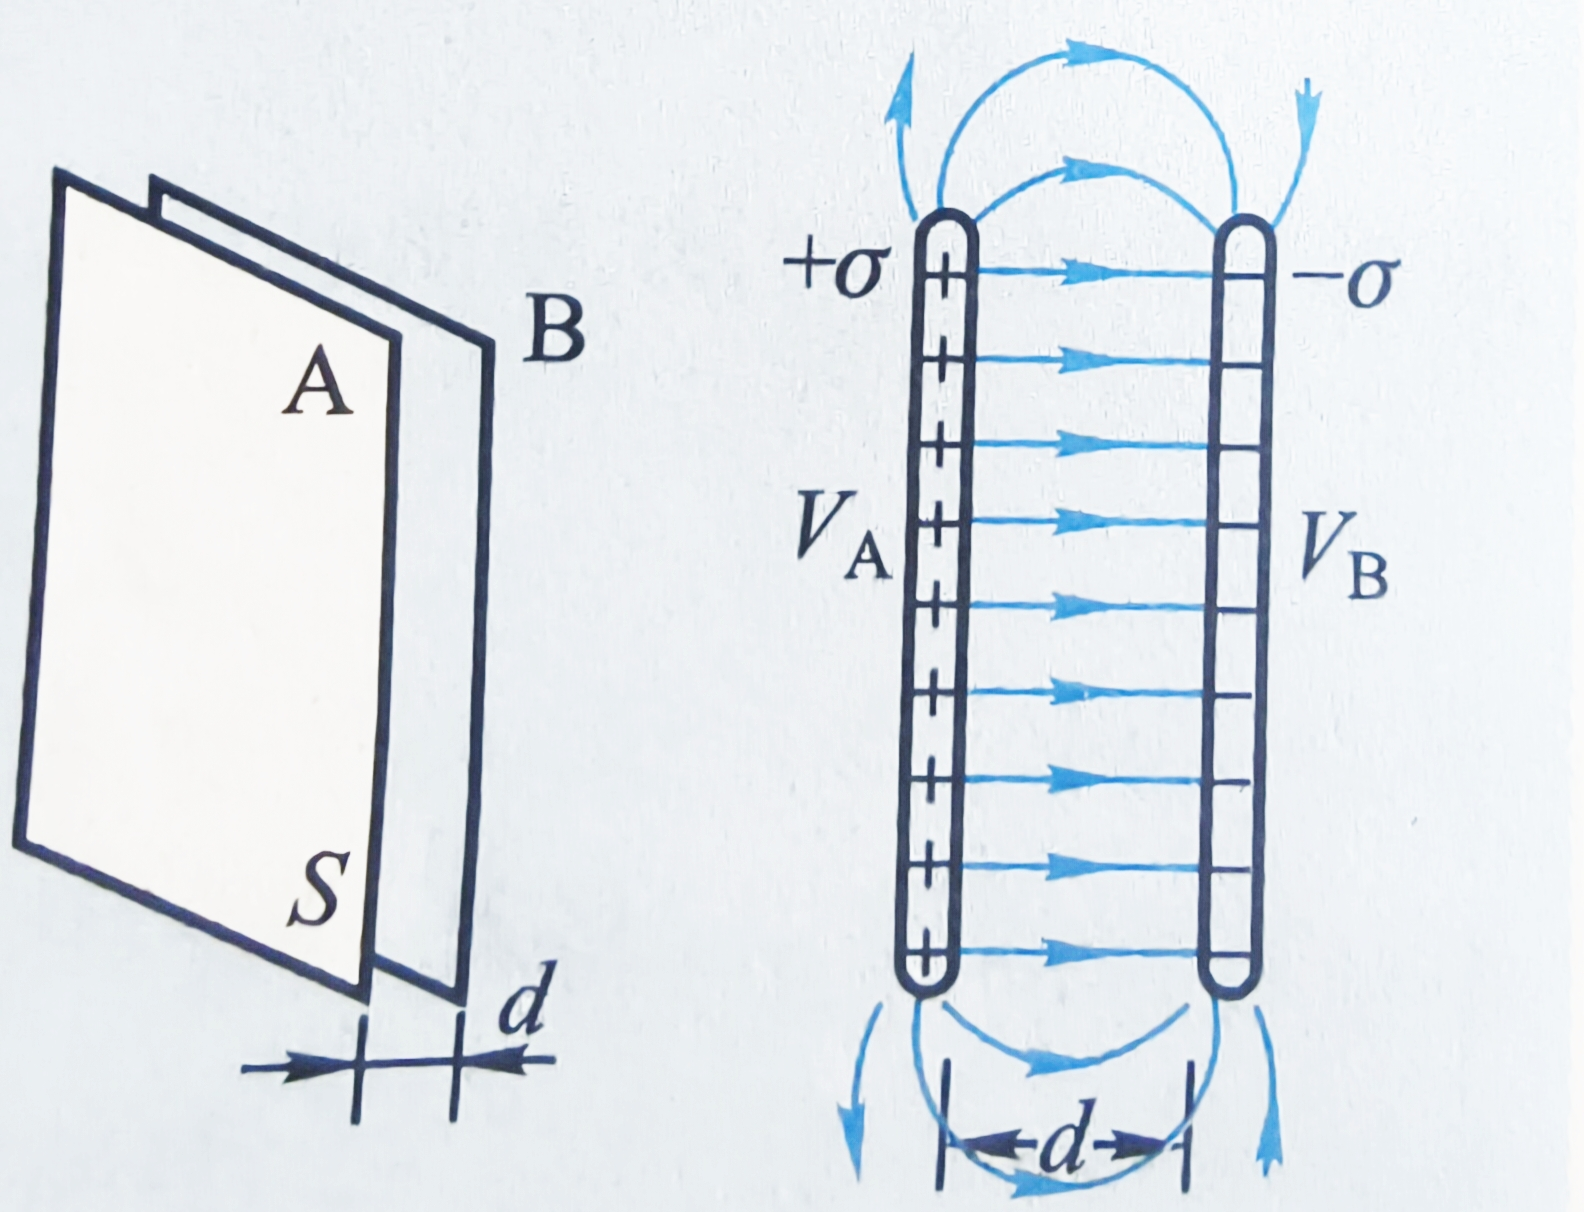
\includegraphics[width=0.4\linewidth]{images/平行板电容器}
	\caption{平行板电容器}
	\label{fig:}
\end{figure}

\subsubsection{同轴圆柱形电容器}

由于两极板距离很近，从两极板中间一点看，可以将其视作无限大带电平面，柱长为L，带电荷量为Q，内半径为$R_{A}$，外半径为$R_{B}$。

设线密度为$\lambda$，$\lambda =\frac{Q}{l}$

取圆柱形高斯面，半径为r,高度为h，则有$$\oint \mathbf{E}\mathrm{d}S=\int_{侧}\mathbf{E}\mathrm{d}S=2\mathbf{E}\pi rh=\frac{\lambda h}{\varepsilon_{0}}$$

求出$$\mathbf{E}=\frac{\lambda}{2\pi\varepsilon_{0}r} $$

则有$$U_{AB}=\int_{R_{A}}^{R_{B}}\mathbf{E}\mathrm{d}r=\int_{R_{A}}^{R_{B}}\frac{\lambda}{2\pi\varepsilon_{0}r}\mathrm{d}r=\frac{\lambda}{2\pi\varepsilon_{0}}\ln\frac{R_{B}}{R_{A}}$$
	
因此$$C=\frac{Q}{U_{AB}}=\frac{2\pi\varepsilon_{0}l}{\ln\frac{R_{B}}{R_{A}}}$$

\begin{figure}[h]
	\centering
	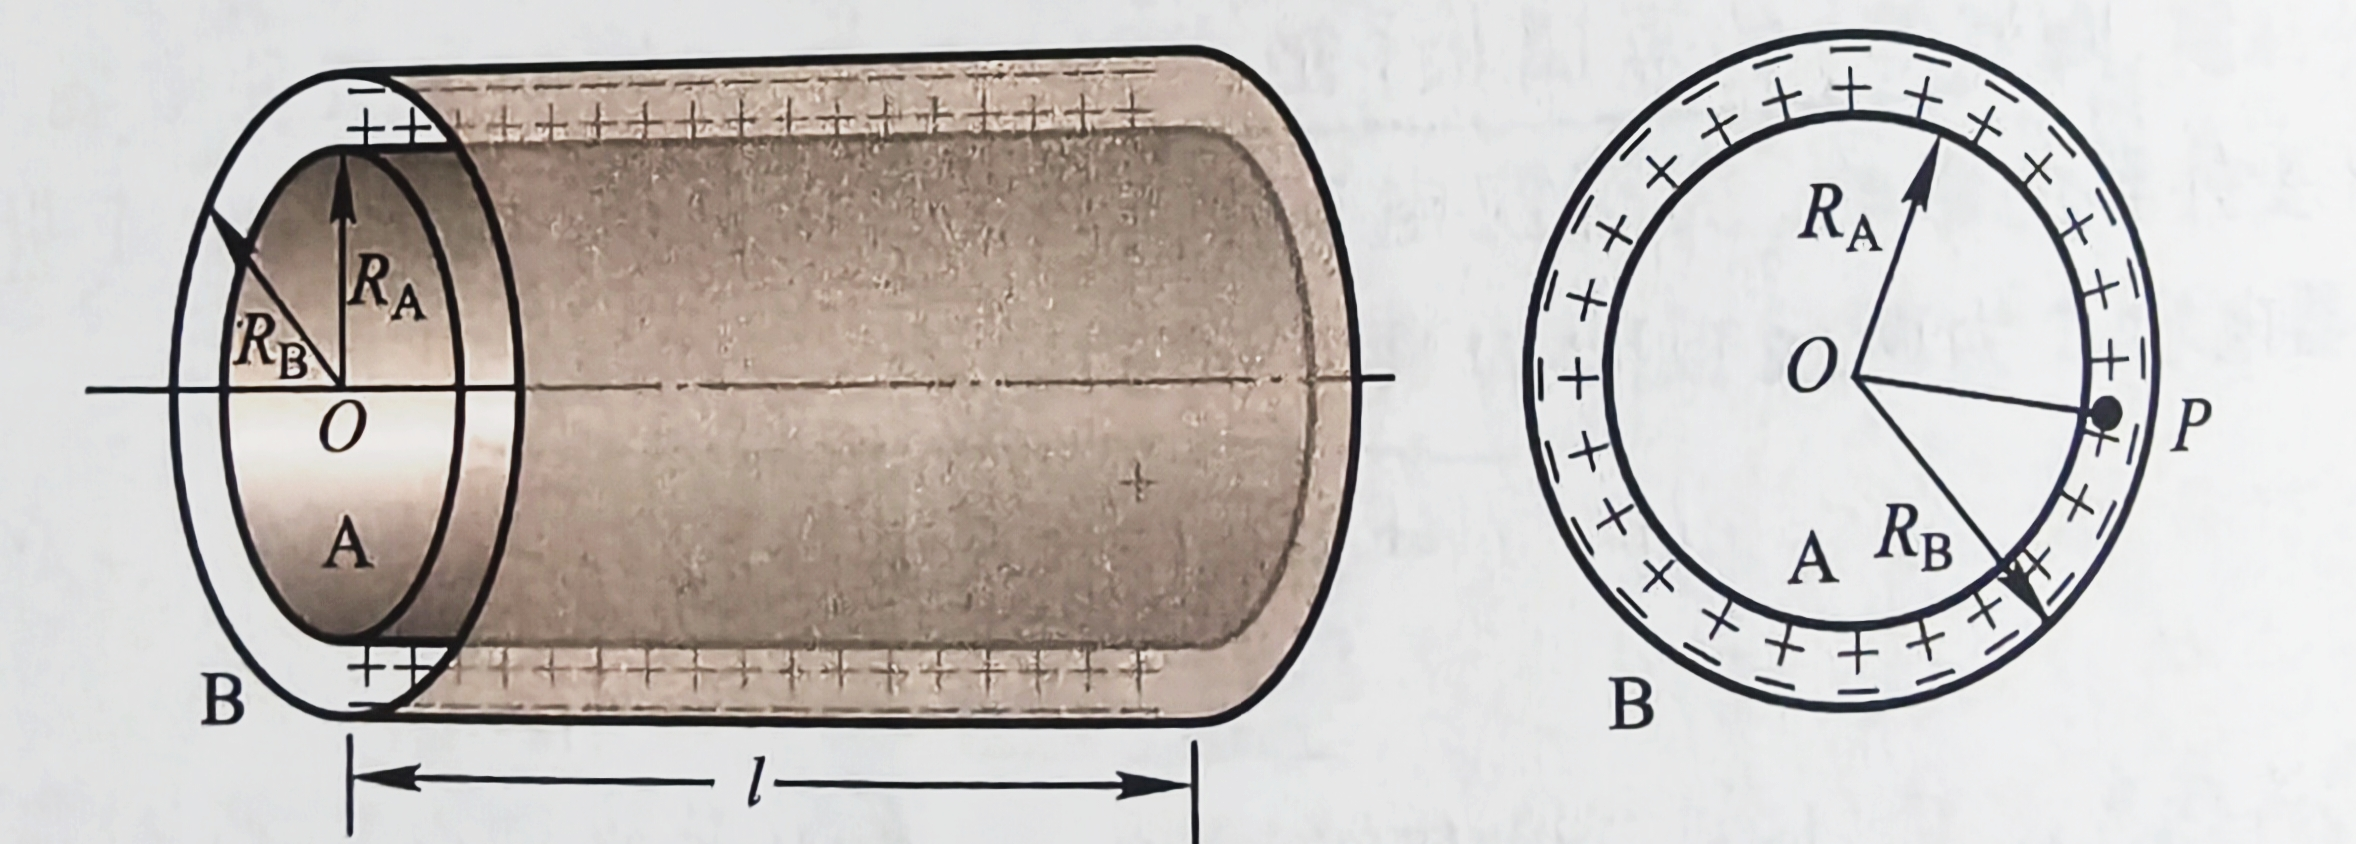
\includegraphics[width=0.5\linewidth]{images/同轴圆柱形电容器}
	\caption{同轴圆柱形电容器}
	\label{fig:}
\end{figure}

\subsubsection{球形电容器}

球形电容器由两个同心的金属球壳组成，内球面半径为$R_{A}$，外球面半径为$R_{B}$，带电荷量为Q。

当$R_{A}<r<R_{B}$时，$$\mathbf{E}=\frac{Q}{4\pi\varepsilon_{0}r^{2}}$$

则$$U_{AB}=V_{A}-V_{B}=\int_{R_{A}}^{R_{B}}\mathbf{E}\mathrm{d}r=\int_{R_{A}}^{R_{B}}\frac{Q}{4\pi\varepsilon_{0}r^{2}}\mathrm{d}r=\frac{Q}{4\pi\varepsilon_{0}}(\frac{1}{R_{A}}-\frac{1}{R_{B}})$$

则$$C=\frac{Q}{U_{AB}}=4\pi\varepsilon_{0}\frac{R_{A}R_{B}}{R_{B}-R_{A}}$$

\begin{figure}[h]
	\centering
	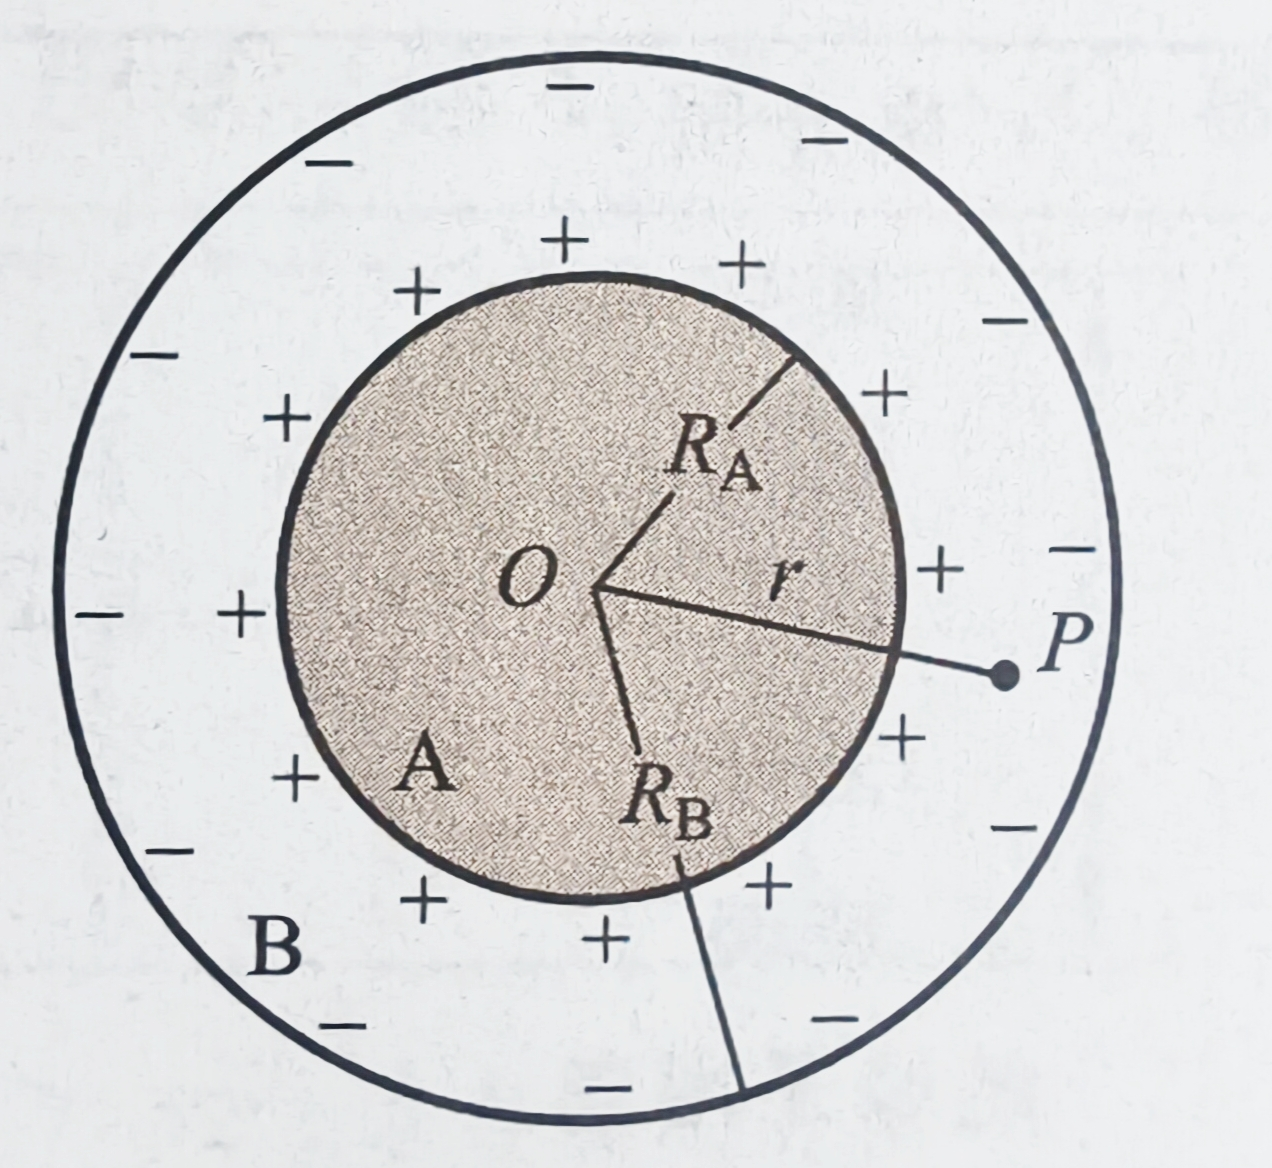
\includegraphics[width=0.4\linewidth]{images/球形电容器}
	\caption{球形电容器}
	\label{fig:}
\end{figure}

\subsection{电容器的串联与并联}

\subsubsection{电容器的串联}

$$C=\frac{Q}{U}=\frac{Q}{U_{1}+U_{2}+U_{3}+......+U_{n}}=\frac{Q}{\frac{Q}{C_{1}}+\frac{Q}{C_{2}}+\frac{Q}{C_{3}}+......+\frac{Q}{C_{n}}}=\frac{1}{\frac{1}{C_{1}}+\frac{1}{C_{2}}+\frac{1}{C_{3}}+......\frac{1}{C_{n}}} $$

\begin{figure}[h]
	\centering
	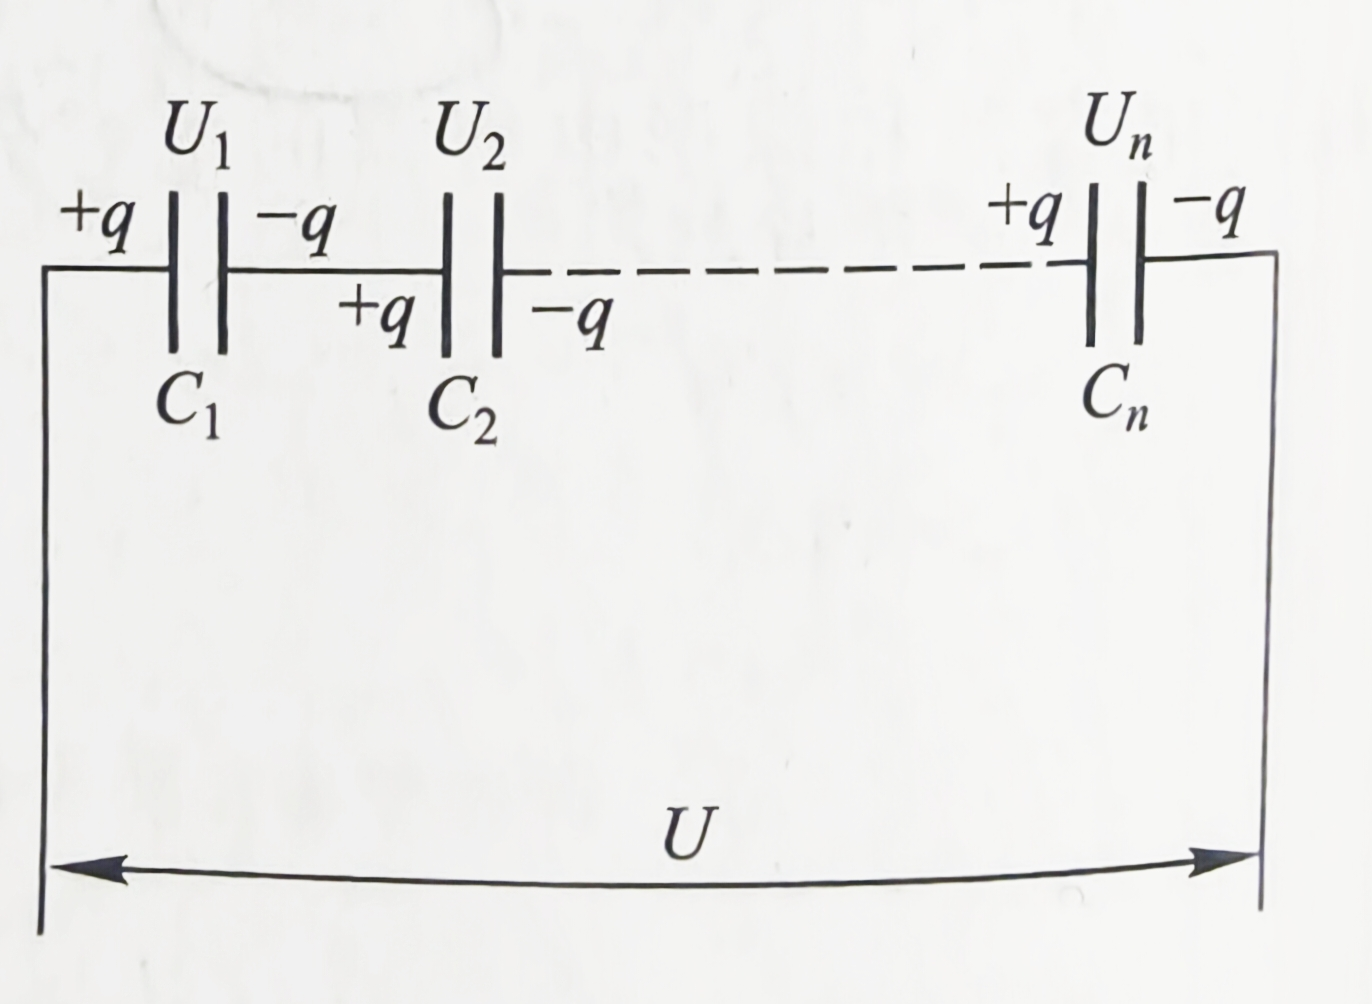
\includegraphics[width=0.4\linewidth]{images/电容器串联}
	\caption{电容器串联}
	\label{fig:}
\end{figure}

\subsubsection{电容器的并联}

$$C=\frac{Q}{U}=\frac{C_{1}U_{1}+C_{2}U_{2}+C_{3}U_{3}+......C_{n}U_{n}}{U} $$

\begin{figure}[h]
	\centering
	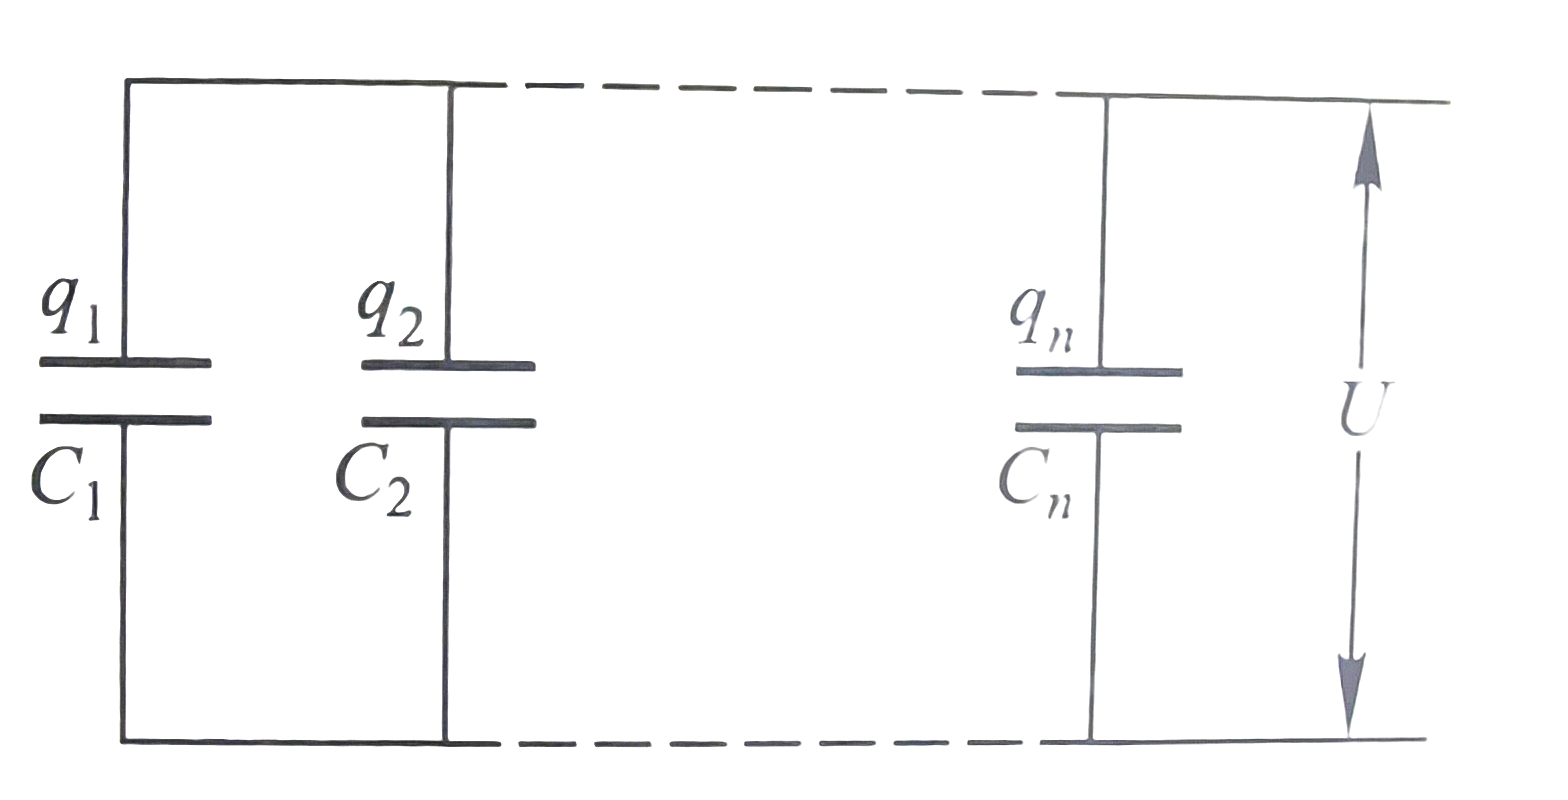
\includegraphics[width=0.5\linewidth]{images/电容器并联}
	\caption{电容器并联}
	\label{fig:}
\end{figure}

\section{静电场中的电介质}
电介质的定义：电介质是电阻率很大，导电性能很差的物质。

电介质的极化：当电介质处在电场中时，电介质中，无论是原子中的电子还是分子中的离子或是晶体晶格上的带电粒子，在电场的作用下都会在原子大小的范围内移动。

当达到静电平衡时，在电介质表面层或体内会出现极化电荷，这个现象称作电介质的极化。

\subsection{电介质的电结构与极化}
\subsubsection{无极分子}
分子内正、负电荷中心重合，等效电偶极矩等于零，电介质整体呈电中性。

无极分子的极化来自正、负电荷中心的相对位移，所以常叫做位移极化。

\subsubsection{极性分子}
分子内正、负电荷中心不相重合。设极性分子的正负电荷中心之间的距离为$l$，分子中全部正电荷或负电荷的总电荷量为$q$，则等效电偶极矩$\vec{p}=q\vec{l}$，电介质整体呈电中性。

极性分子的极化就是等效电偶极子转向外电场的方向，叫做取向极化（一般来说，分子在取向极化的同时还会产生位移极化，但极性分子电介质以取向极化为主）。

\subsubsection{极化后电介质中的电荷分布}
如果电介质是均匀的，则在它内部仍然保持电中性，但是在电介质的两个和外电场强度$\vec{E_0}$相垂直的表面层里（厚度为分子等效电偶极矩的轴长$l$），将会分别出现正电荷和负电荷。

\subsection{电极化强度}
两类电介质极化的微观过程虽然不同，但宏观的效果却是相同的。都是在电介质的两个相对表面上出现了异号的极化电荷，在电介质内部有沿电场方向的电偶极矩。

我们取单位体积内分子电偶极矩的矢量和，即
$$\vec{P}=\frac{\sum \vec{p}}{\Delta V}$$
作为量度电介质极化程度的基本物理量，称为该点的电极化强度或$\vec{P}$矢量。单位是$C/m^2$。

\subsection{电极化强度与极化电荷的关系}
对于均匀电介质，其极化电荷只集中在表面层里或在两种不同的界面层里。

设$\vec{e_n}$为介质表面的单位法向矢量，那么
$$\sigma'=\vec{P}\cdot\vec{e_n}=P_n$$
即介质极化所产生的极化电荷面密度等于电极化强度沿介质表面外法线的分量。

\subsection{介质中的静电场}
\subsubsection{物理量}
电介质的电极化率：$\chi_e$，和电介质的性质有关，量纲为1。

电介质的相对电容率：$\varepsilon_r$

电介质的电容率/介电常量：$\varepsilon$

\subsubsection{公式}
对于各向同性电介质，有：

$\vec{E}=\vec{E_0}+\vec{E'}$

$\vec{P}=\chi_e\varepsilon_0\vec{E}$

$\varepsilon_r=1+\chi_e$

$\varepsilon=\varepsilon_r\varepsilon_0=(1+\chi_e)\varepsilon_0$

\subsubsection{（特例：平行板电容器）}
除满足以上公式外，还有

$E_0=\sigma_0/\varepsilon_0$

$E'=\sigma'/\varepsilon_0$

$E=\frac{E_0}{1+\chi_e}$

\subsubsection{拓展：非各向同性电介质}
自然界也存在一些电介质，在一定的温度范围内电容率随电场强度而变化，它们的极化规律有着复杂的线性关系。

如铁电体、永驻体、压电效应、电致伸缩等。

	
	
	\section{有电介质时的高斯定理和环路定理  电位移}
	
	
	\begin{definition}[电位移]
		电位移用$D$表示，单位是$C/m^2$。
		$$D = \varepsilon_{0}E + P$$
		其中，$P$为电极化强度。
	\end{definition}
	
\begin{definition}[电位移通量]
在有电介质的静电场中作电位移线，使线上每一点的切线方向和该点电位移 D 的方向相同，并规定在垂直于电位移线的单位面积上通过的电位移线数目等于该点的电位移 D 的量值，被称为称作电位移通量。
\end{definition}
	
	\begin{definition}[有电介质时的高斯定理]
		$$\oint_{S} D \cdot dS = q_{0}$$
	\end{definition}
	
\begin{note}
有电介质时的高斯定理是静电场基本定理之一，是普遍适用的。
	
通过电介质中任一闭合曲面的电位移通量，等于该面所包围的自由电荷量的代数和。

电位移线是从正的自由电荷出发，终止于负的自由电荷（不包括极化电荷）。

\end{note}
	
	
\begin{note}
$D$和$E$和$P$的关系和区分：

有电介质时，平行板电容器之间$D$线均匀分布（从正的自由电荷出发，终止于负的自由电荷）（不包括极化电荷），$E$线有部分终止于极化电荷，在电介质内较为疏松，$P$线起始于负极化电荷，终止于正极化电荷，只在电介质内部。

设电极化率为$\chi_{e}$，相对电容率$\varepsilon_{0}$，电容率$\varepsilon$
$$D = \varepsilon_{0}E + P = \varepsilon_{0}E + \chi_{e}\varepsilon_{0}E = \varepsilon_{r}\varepsilon_{0}E$$
	$$D = \varepsilon E$$
		
\end{note}
	
	\begin{definition}[有电介质时的环路定理]
$$\oint_{L} E \cdot dl = 0$$
$E$为所有电荷激发的静电场。
	\end{definition}
\begin{supplement}
带电金属球周围充满均匀无限大电介质后，其电场强度减弱到真空时的$\frac{1}{\varepsilon_{r}}$
\end{supplement}

\begin{supplement}
$E = \frac{E_{0} }{\varepsilon_{r}}$ 和 $D = \varepsilon_{0}E $仅在均匀电介质充满整个电场或电介质表面是等势面时成立。
\end{supplement}
	

	

\chapter{静磁场}
\section{毕奥-萨伐尔定律}
\subsection{毕奥-萨伐尔定律}
电流元$I\mathbf{d}\vec{l}$在空间任一点P处所激发磁场的磁感应强度为
$$\mathbf{d}\vec{B}=\frac{\mu_0}{4\pi}\frac{I\mathbf{d}\vec{l}\times\vec{e_r}}{r^2}$$

电流元：用矢量$I\mathbf{d}\vec{l}$表示。其中$\mathbf{d}\vec{l}$表示在载流导线上（沿电流方向）所取的线元，$I$为导线中的电流，电流元的方向规定为电流沿线元的流向。

$\mu_0=4\pi\times10^{-7}T\cdot m/A$，称为真空磁导率。

$\vec{e_r}$是从电流元所在处到场点$P$的位矢。

\subsection{应用示例}
\subsubsection{载流直导线}
对于长为$L$的载流直导线，距离直导线为$a$的$P$点的磁感应强度：
$$B=\frac{\mu_0 I}{4\pi a}(\sin\beta_2-\sin\beta_1)$$
\begin{figure}[h]
	\centering
	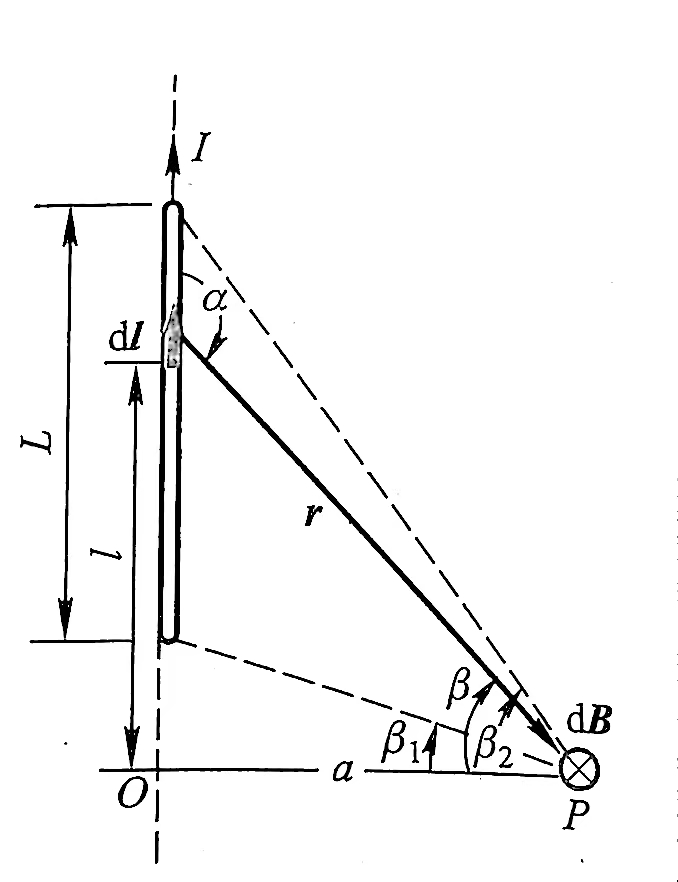
\includegraphics[width=0.3\textwidth]{images/8.3 载流直导线.jpg}
	\caption{载流直导线附近磁场的计算}
\end{figure}

对于无限长载流直导线，取$\beta_1=-\pi/2$，$\beta_2=\pi/2$，得：
$$B=\frac{\mu_0 I}{2\pi a}$$

\subsubsection{载流圆线圈的轴线}
$$B=\frac{\mu_0}{2\pi}\frac{IS}{(R^2+x^2)^{3/2}}$$
\begin{figure}[h]
	\centering
	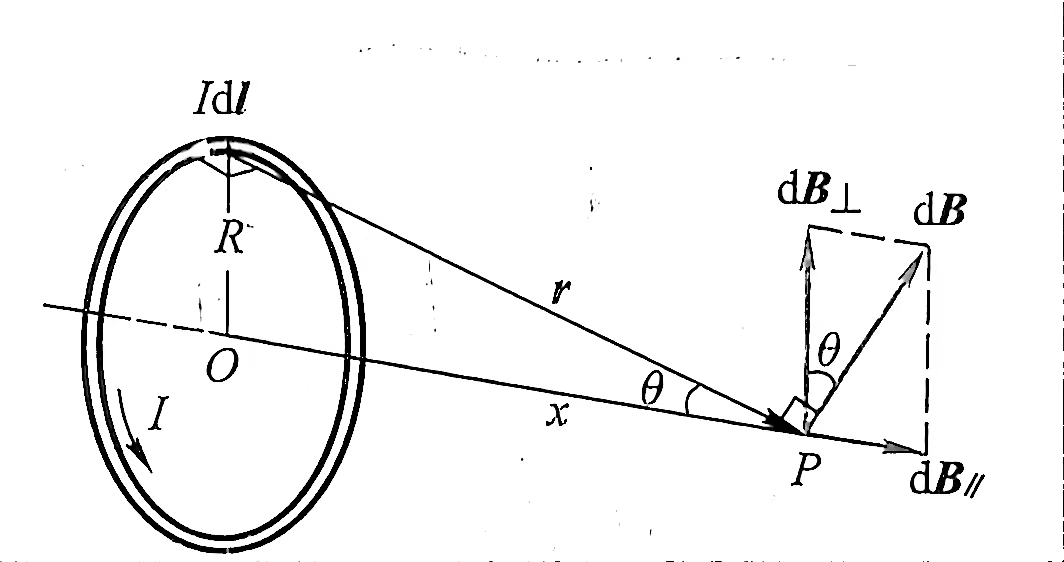
\includegraphics[width=0.5\textwidth]{images/8.3 圆电流轴线.jpg}
	\caption{圆电流轴线上磁场的计算}
\end{figure}

在圆心$x=0$处，$B_0=\frac{\mu_0I}{2R}$

当$x\gg R$时，$B=\frac{\mu_0IS}{2\pi x^3}$

引入磁矩$\vec{m}=IS\vec{e_n}$（若线圈有$N$匝，则磁场加强$N$倍，$\vec{m}=NIS\vec{e_n}$），其中$\vec{e_n}$表示线圈平面法线方向的单位矢量（由线圈中电流流向按右手螺旋定则确定）。则：
$$\vec{B}=\frac{\mu_0\vec{m}}{2\pi x^3}$$
\begin{figure}[h]
	\centering
	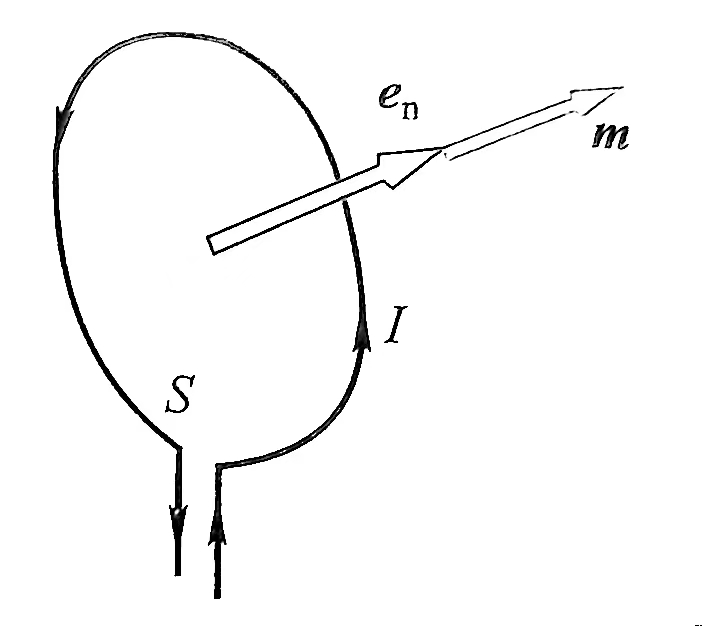
\includegraphics[width=0.3\textwidth]{images/8.3 磁矩.jpg}
	\caption{磁矩的方向}
\end{figure}

\subsubsection{载流直螺管内部}
\begin{figure}[h]
	\centering
	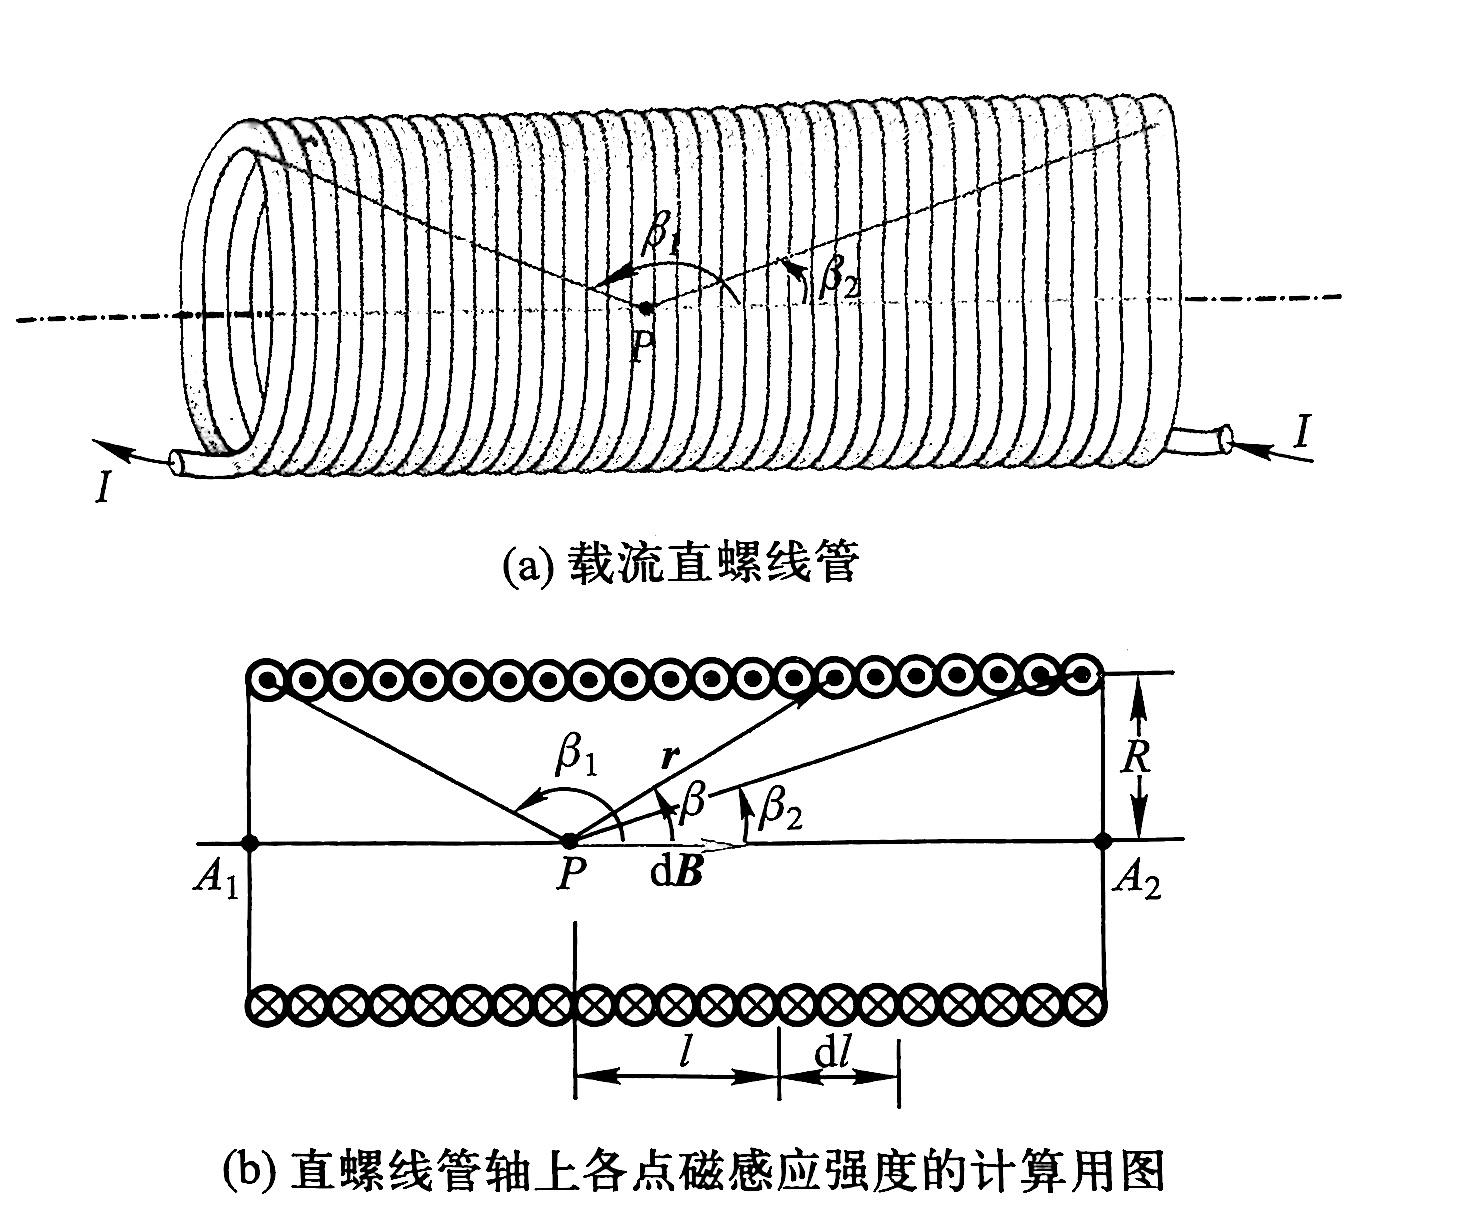
\includegraphics[width=0.5\textwidth]{images/8.3 直螺线管内部.jpg}
	\caption{直螺线管内部磁场的计算}
\end{figure}
螺线管半径为$R$，电流为$I$，每单位长度有线圈$n$匝：
$$B=\frac{\mu_0}{2}nI(\cos\beta_2-\cos\beta_1)$$

无限长螺线管，亦即螺线管的长度$\gg$其直径时：
$$B=\mu_0 nI$$

长螺线管的端点：
$$B=\frac{1}{2}\mu_0 nI$$

\subsection{运动电荷的磁场}
每一个以速度$v$运动的电荷所激发磁场的磁感应强度$B_q$为：
$$B_q=\frac{\mu_0}{4\pi}\frac{q\vec{v}\times\vec{e_r}}{r^2}$$
\section{恒定磁场的高斯定理与安培环路定理}

\subsection{恒定磁场的高斯定理}

1.\textbf{通过任意闭合曲面的磁通量总等于零。}
即$$\oint_{S}\mathbf{B}\mathrm{d}S=0$$

2.激发静电场的场源（电荷）是电场线的源头或尾闾，所以静电场是属于发散状的场，可称作有源场；而磁场的磁感应线无头无尾，永远是闭合的，所以磁场可称作无源场。

3.磁场的高斯定理与静电场的高斯定理不对称的根本原因是自然界不存在单
个磁极（即磁单极子）。

\subsection{恒定磁场的安培环路定理}

1.\textbf{在恒定磁场中，磁感应强度治任一闭合路径的线积分等于$\mu_{0}$倍的穿过以闭合曲线为边界的任意曲面的各恒定电流的代数和,也称为矢量的环流}
即$$\oint\mathbf{B}\mathrm{d}\mathbf{l}=\mu_{0}\sum I_{i}$$

2.通常把磁场叫做有旋场，而$\mathbf{E}$的环流恒等于零，所以把静电场叫做无旋场。

3.讨论:

(1)B是空间全部电流产生的磁场。

(2)对任意形式的恒定电流所激发的磁场都成立，对任何形形状的闭合路径都成立。

\subsection{典型安培环路定理的应用}

\subsubsection{无限长直电流的磁场}

\begin{figure}[h]
	\centering
	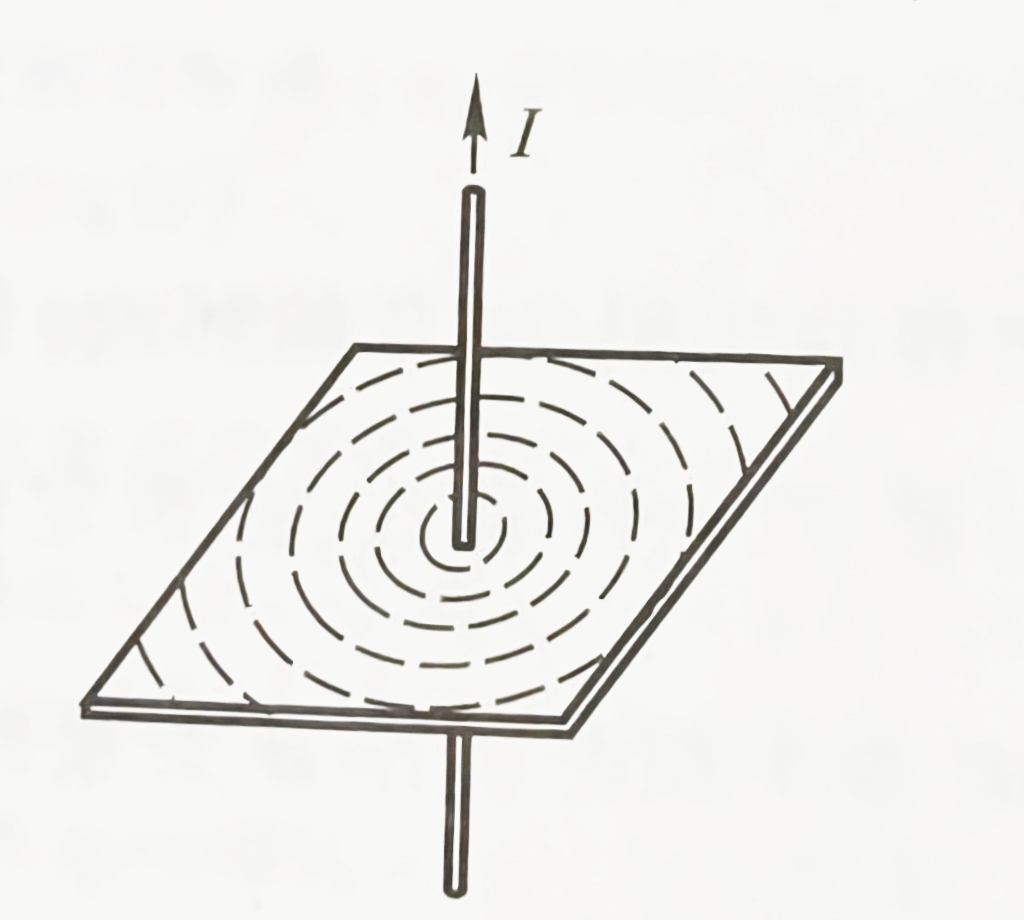
\includegraphics[width=0.4\linewidth]{images/无限长直导线的磁场}
	\caption{无限长直导线的磁场}
	\label{fig:}
\end{figure}

磁场为一圈一圈的同心圆，取闭合路径为磁场的同心圆，半径为r。

由安培环路定理$$ \oint\mathbf{B}\mathrm{d}\mathbf{l}=\oint B\mathrm{d}l=B\oint\mathrm{d}l=\mu_{0}\sum I_{i}$$

则$$2B\pi r=\mu_{0}I$$
$$B=\frac{\mu_{0}I}{2\pi r}$$

方向与电流流向呈右手螺旋定则

\subsubsection{长直圆柱形载流导线内外的磁场}

\begin{figure}[h]
	\centering
	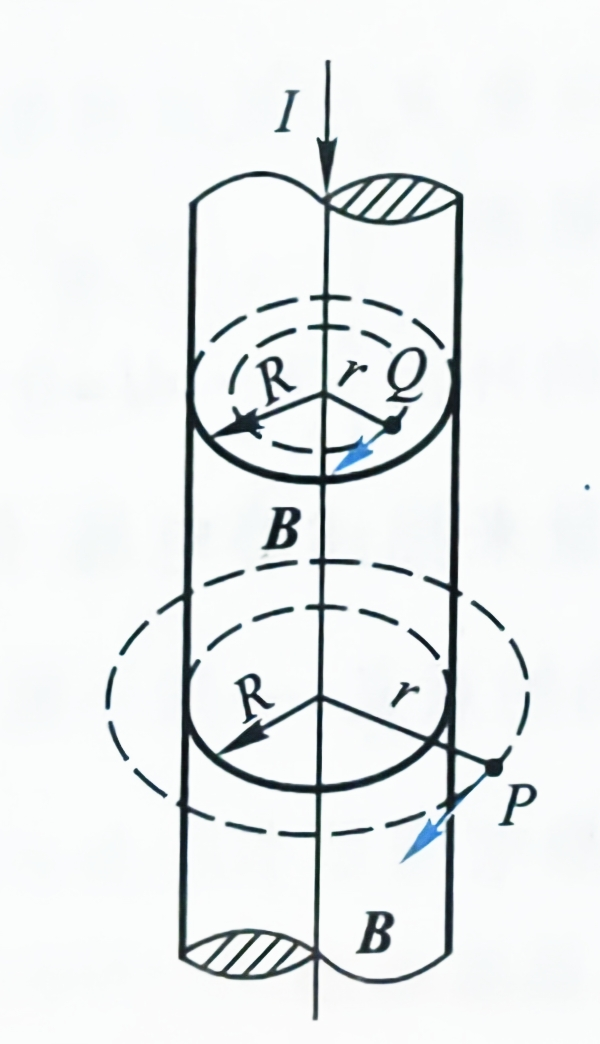
\includegraphics[width=0.2\linewidth]{images/长直圆柱形载流导线内外的磁场}
	\caption{长直圆柱形载流导线内外的磁场}
	\label{fig:}
\end{figure}

从轴线方向看，上下左右对称的电流对圆柱形载流导线外一点的磁感应强度是对称的，因此磁场呈轴对称分布，磁感应线为垂直于轴线的同心圆。

圆柱的半径为R，取半径为r的同心圆为闭合路径。

则由安培环路定理$$\oint\mathbf{B}\mathrm{d}\mathbf{l}=\oint B\mathrm{d}l=B\oint\mathrm{d}l=\mu_{0}\sum I_{i} $$

1.当r>R时，则$$2B\pi r=\mu_{0}I$$

2.当r<R时，则$$2B\pi r=\mu_{0}\frac{\pi r^{2}}{\pi R_{^{2}}}$$

则$$\left\{
\begin{aligned}
	B&=\frac{\mu_{0}I}{2\pi r}，,r>R\\
	B&=\frac{\mu_{0}Ir}{2\pi R}，,r<R
\end{aligned}
\right.$$

\subsubsection{均匀密绕无限长直螺线管的磁场}

\begin{figure}[h]
	\centering
	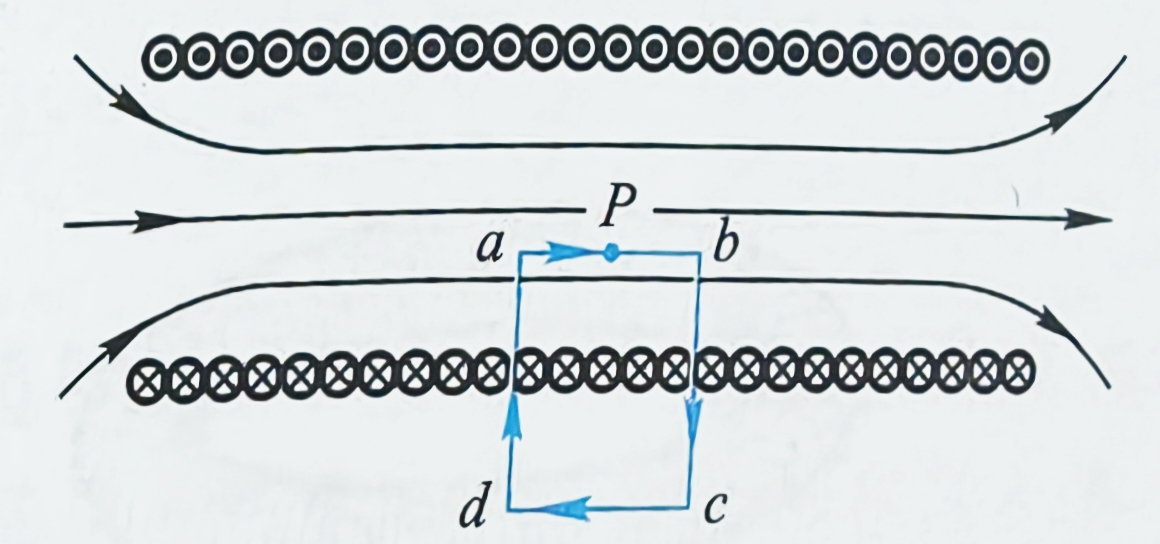
\includegraphics[width=0.5\linewidth]{images/均匀密绕无限长直螺线管的磁场}
	\caption{均匀密绕无限长直螺线管的磁场}
	\label{fig:}
\end{figure}

已知有N匝线圈，电流为I，数密度为n。

P为螺线管内一点，由分析可知，P点磁感线的方向为过点P且平行于轴线的方向，该同一直线上其他点方向也沿该直线。即\textbf{P点所在的平行直线上大小相同，方向相同}

取闭合回路为矩形abcda

则由安培环路定理$$\oint\mathbf{B}\mathrm{d}\mathbf{l}=Bl_{ab}=\mu_{0}nl_{ab}I$$

则$$B=\mu_{0}nI $$

在螺线管外部，磁感线相互抵消，磁感应强度很小，$B_{内}\gg B_{外}$，可视做$B_{外}=0 $，所以多匝线圈一般被视为储能原件。

\subsubsection{均匀载流螺绕环的磁场}

\begin{figure}[h]
	\centering
	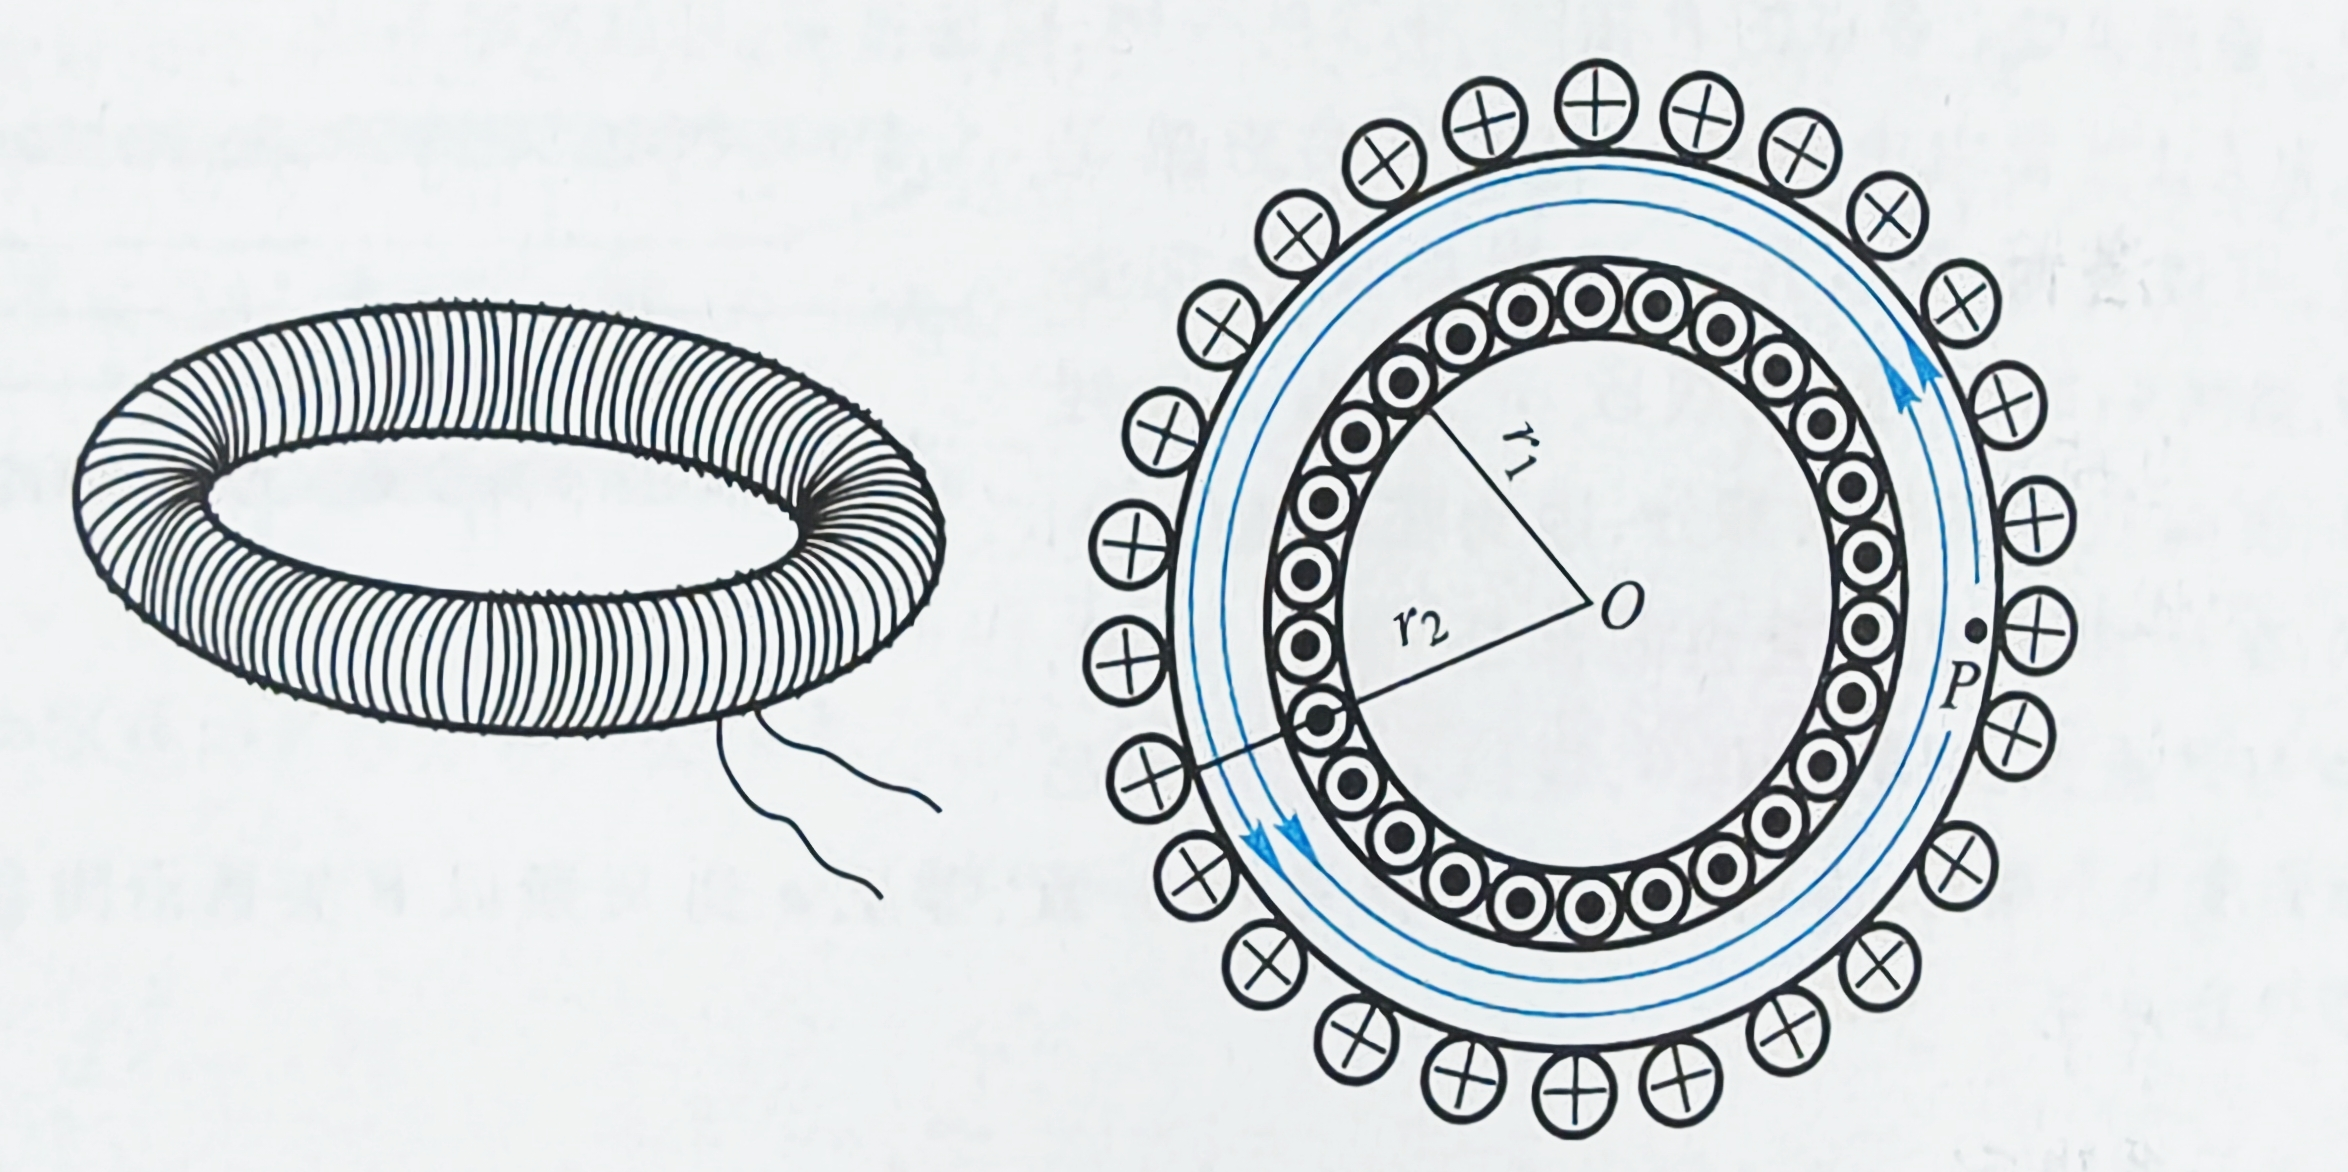
\includegraphics[width=0.6\linewidth]{images/均匀载流螺绕环的磁场}
	\caption{}
	\label{fig:}
\end{figure}

已知内径为$R_{1}$，外径为$R_{2}$，电流为I，匝数为N。

经放大图分析，螺绕环的磁感线为其内部的同心圆，取半径为r的同心圆为闭合路径。

则由安培环路定理$$\oint\mathbf{B}\mathrm{d}\mathbf{l}=\oint B\mathrm{d}l=B\oint\mathrm{d}l=\mu_{0}\sum I_{i} $$

1.当$R_{1}$<r<$R_{2}$时，则$$2B\pi r=\mu_{0}NI$$

2.当r>$R_{2}$时，电流相互抵消，则$$2B\pi r=0$$

则$$\left\{
\begin{aligned}
	B&=\frac{\mu_{0}NI}{2\pi r},R_{1}<r<R_{2}\\
	B&=0,r>R_{2}
\end{aligned}
\right.$$
\section{铁磁质}
概括起来说，铁磁质有下列一些特殊的性质：
\begin{enumerate}
	\item 能产生特别强的附加磁场$B'$，使铁磁质中的$B$远大于$B_0$,其$\mu_r=B/B_0$可达几百、甚至几千。
	\item 它们的磁化强度$M$和磁感应强度$B$不再是常矢量，没有简单的正比关系，其磁导率$\mu$（以及磁化率$\chi_m$）与磁场强度$H$的函数关系比较复杂。
	\item 磁化强度随外磁场而变，它的变化落后于外磁场的变化，而且在外磁场停止作用后，铁磁质仍能保留部分磁性。
	\item 一些铁磁质存在一特定的临界温度，称为居里点（Curie point)，在温度达到居里点后，它们的磁性发生突变，转化为顺磁质，磁导率（或磁化率）和磁场强度$H$无关。例如，铁的居里点是1040$K$，镍的是631$K$，钻的是1388$K$。
\end{enumerate}
\chapter{电磁感应}
\section{磁场的能量}
\subsection{推导}
设电路接通后回路中某瞬时的电流为$I$，自感电动势为$-L\mathbf{d}I/\mathbf{d}t$，由回路的欧姆定律得
$$\varepsilon-L\frac{\mathbf{d}I}{\mathbf{d}t}=IR$$
$$\int_{0}^{t}\varepsilon I\mathbf{d}t=\int_{0}^{I_0}LI\mathbf{d}I+\int_{0}^{t}R^2I^2\mathbf{d}I$$

在自感与电流无关的情况下，得到
$$\int_{0}^{t}\varepsilon I\mathbf{d}t=\frac{1}{2}LI_0^2+\int_{0}^{t}R^2I^2\mathbf{d}I$$

说明电源电动势所做的功转化为两部分能量。其中$\int_{0}^{t}R^2I^2\mathbf{d}I$是$t$时间内消耗在电阻$R$上的焦耳热；$\frac{1}{2}LI_0^2$是回路中建立电流的变化过程中电源电动势克服自感电动势所做的功，也就是储存在磁场中的能量。
\subsection{结论}
\subsubsection{磁场的能量}
一个自感为$L$的回路，当其中通有电流$I_0$时，其周围空间磁场的能量为
$$W_m=\frac{1}{2}LI_0^2$$

\subsubsection{磁场能量密度}
在一般情况下，磁场能量密度可以表达为
$$w_e=\frac{1}{2}\vec{B}\cdot\vec{H}$$

若磁场是不均匀的，则：
$$W_m=\int_{V}w_m\mathbf{d}V=\frac{1}{2}\int_{V}\vec{B}\cdot\vec{H}\mathbf{d}V$$

由$\frac{1}{2}LI_0^2=\frac{1}{2}\int_{V}\vec{B}\cdot\vec{H}\mathbf{d}V$，可求出回路的自感。

\end{document}